\documentclass{book}
\author{David Corzo}
\date{22/07/2019}
\title{Economía II}
%%%%%%%%%%%%%%%%%%%%%%%%%%%%%%%%%%%%%%%%%%%%%%%%%%%%%%%%%%
\usepackage[margin=1in]{geometry}
\usepackage{graphicx}
\usepackage{fontenc}
\usepackage[spanish]{babel}
\usepackage{amsmath}
\usepackage{amsthm}
\usepackage[utf8]{inputenc}
\usepackage{enumitem}
\usepackage{mathtools}
\usepackage{import}
\usepackage{xifthen}
\usepackage{pdfpages}
\usepackage{transparent}
\usepackage{color}
\usepackage{array}
\usepackage{booktabs}
\usepackage{etaremune}
\usepackage{bookmark}
\usepackage{pdfpages}
\usepackage{eurosym}
%%%%%%%%%%%%%%%%%%%%%%%%%%%%%%%%%%%%%%%%%%%%%%%%%%%%%%%%%%


\begin{document}
\maketitle
\tableofcontents

\part{Clases, notas de clases}

\chapter{2019-07-22}
\section{API's \& sus peculiaridades}
\begin{itemize}
\item \textbf{Nos preguntamos:} ¿Por que razón puedo ver el XML en el browser? Es por que estamos usando el método GET.
\item AJAX no permite no tiene la versitabilidad de parser. Este es el defecto de beautiful Soup, para el tipo de interacciónes con AJAX se necesita usar elenioum.
\end{itemize}

\section{Flask}
\begin{itemize}
    \item Flase es un framework, no es como Django que uno es obligado a usar cirtas cosas oblgatoriamente, \emph{\textbf{Definición de ``framework":} es un set de herramientas.}
    \item Usualmente utiliza menos memoria usar ``from <librería> import <funciones o clases a usar>''.
    \item Está corriendo en un puerto.
    \item \emph{\textbf{Definición de ``Socket":} la combinación de una IP  y un puerto}.
    \item Con hostname:
    \begin{verbatim}
        DAVIDCORZO@DESKTOP-73D7DE2 /cygdrive/c/Users/DAVIDCORZO
        $ hostname
            DESKTOP-73D7DE2
    \end{verbatim}
    
    \item app.run(host$=$"0.0.0.0",port=55) el host= 0.0.0.0. permite ver por medio de la red aplicaciones corriendo en otras computadoras.
    \item \emph{\textbf{Definición de ``puerto":} permite cambiar el socket, tiene un máximo de 65,535 puertos}.
    \item Debug igual True, uno de los beneficios que permite es correr la app sin tener que iterar el ciclo guardar,correr,ver\_resultados, pero el chiste es debugging.
    \item En python ``@'' es un decorador, es una manera implicia de llamar funciones.
    \item Cambiémos la ruta con el decorador a ``@app.route("/alumnos)''
    \item En flask hay dos formas de render: \emph{\textbf{Definición de ``Server side rendering":} fui a la base de datos y la respuesta solo al sabe mi aplicación, soy capaz por ende de imprimir información ingresada en mi aplicación.} \emph{\textbf{Definición de ``client side rendering":} este render lo hace el browser.}
    \item Lenguages de renderización, pintar de manera bonita en el browser.
    
    \item In jinja2 se referencia a una variable asi: ``\{\{ <variable> \}\}'', para hacer un for loop \{\% for i in algo \%\}.
\end{itemize}

\section{Averiguar después}
\begin{enumerate}
    \item decorators ``@''
    \item CSS Bootstrap
    \item jinja2 en Flask 
    \item Server side render, client side render.
    \item Leer Redis.
\end{enumerate}


\chapter{2019-07-24}
\section{Subjetivismo}
Es la teoría de valor de acuerdo a lo subjetivo, el comunista piensa que el valor de los bienes son objetivos, un comunista pretende planear todo desde arriba. \newline 
Valor de los bienes es subjetivo, bienes tienen función de acurdo necesidades que satisfacen, tiene valor para alguien y para otra persona pueda que no tenga valor. Si la teoría del valor fuese cierta ninguna empresa quebraría. Si la cantidad de trabajo determina el precio simplemente cualquiera quisiera meterle hasta trabajo de por gusto. \newline 
Teoría de subjetivismo: el valor se determina por qué tan bien satisfacen las necesidades existentes.

\section{Marginalismo}
El marginalismo, la paradoja de el agua y los diamantes, las necesidades o el valor de los bienes viene dado de la necesidad marginal, el ultimo de los fines que permite conseguir, toda decisión se toma al margen. El valor que tiene la unidad, la ultima unidad de algún bien.

\begin{center}
    \begin{figure}[htbp]
        \centering
        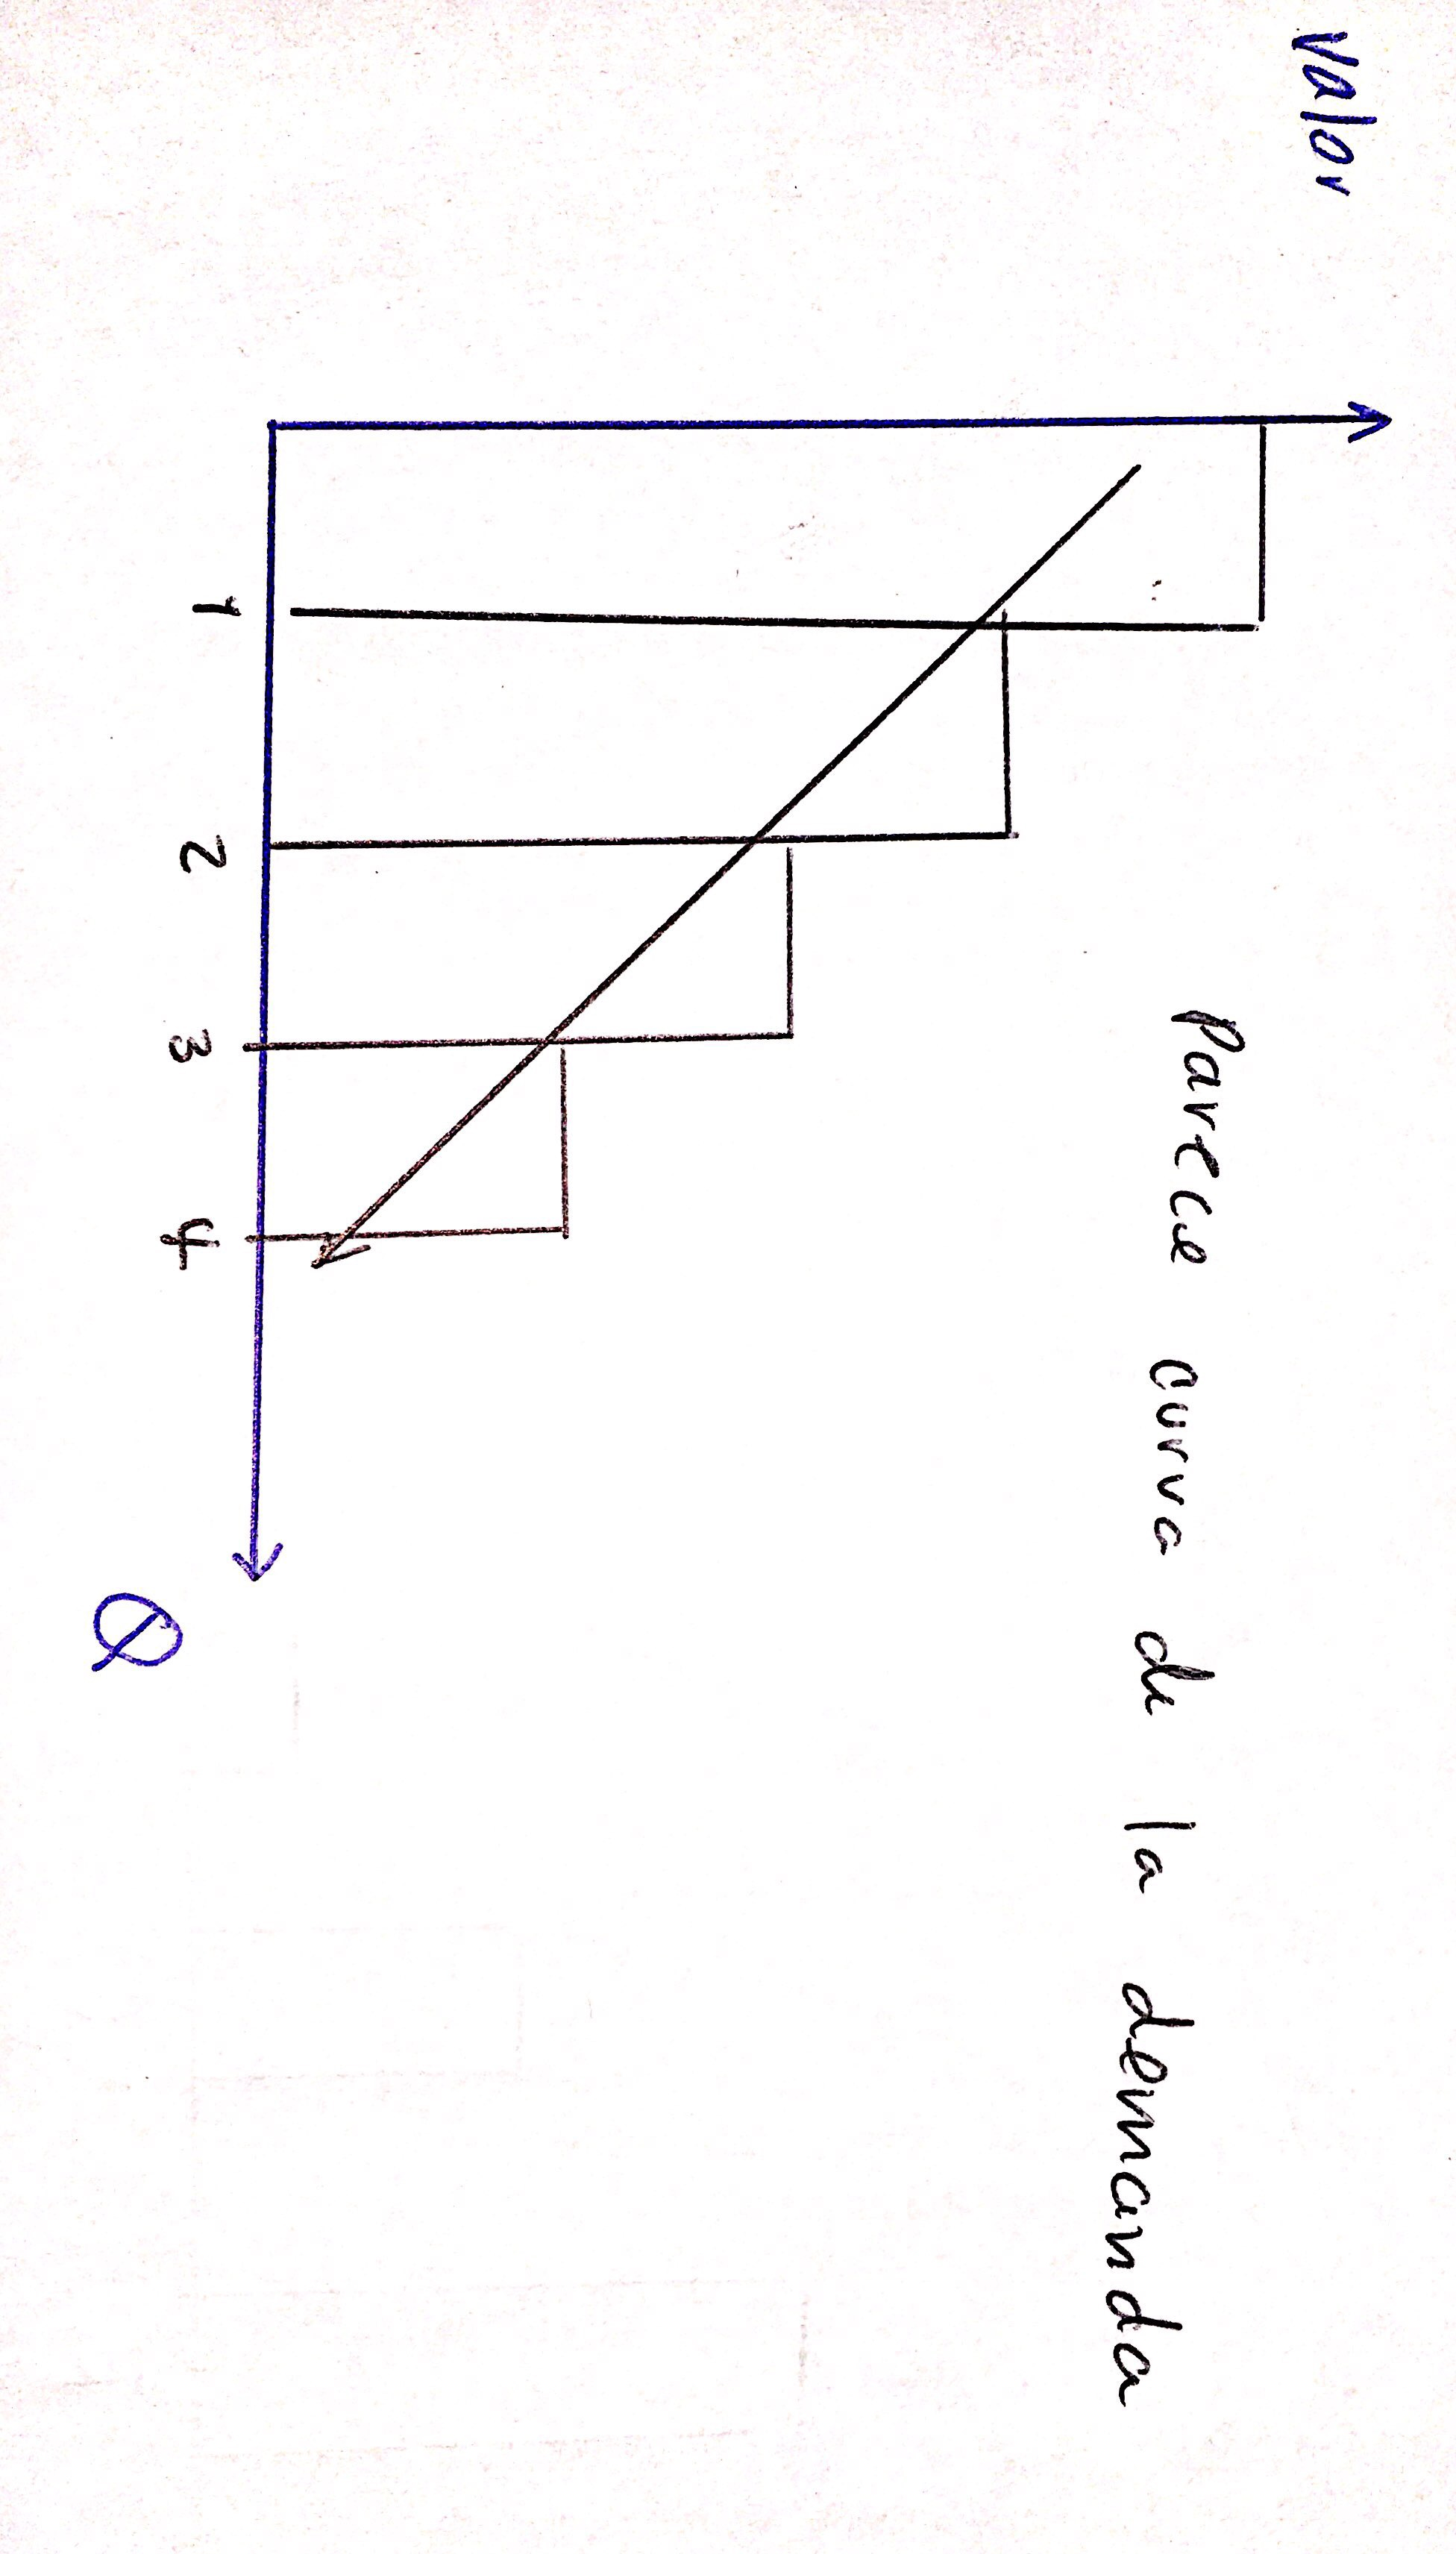
\includegraphics[width=6cm,angle=90]{Classes/Images/2019-07-24-1.jpg}
        \caption{La marginalidad tambien se puede representar como una curva de demanda también}
        \label{fig1}
    \end{figure}
\end{center}

% \vspace{10pt}
\begin{center}
    \begin{figure}[htbp]
        \centering
        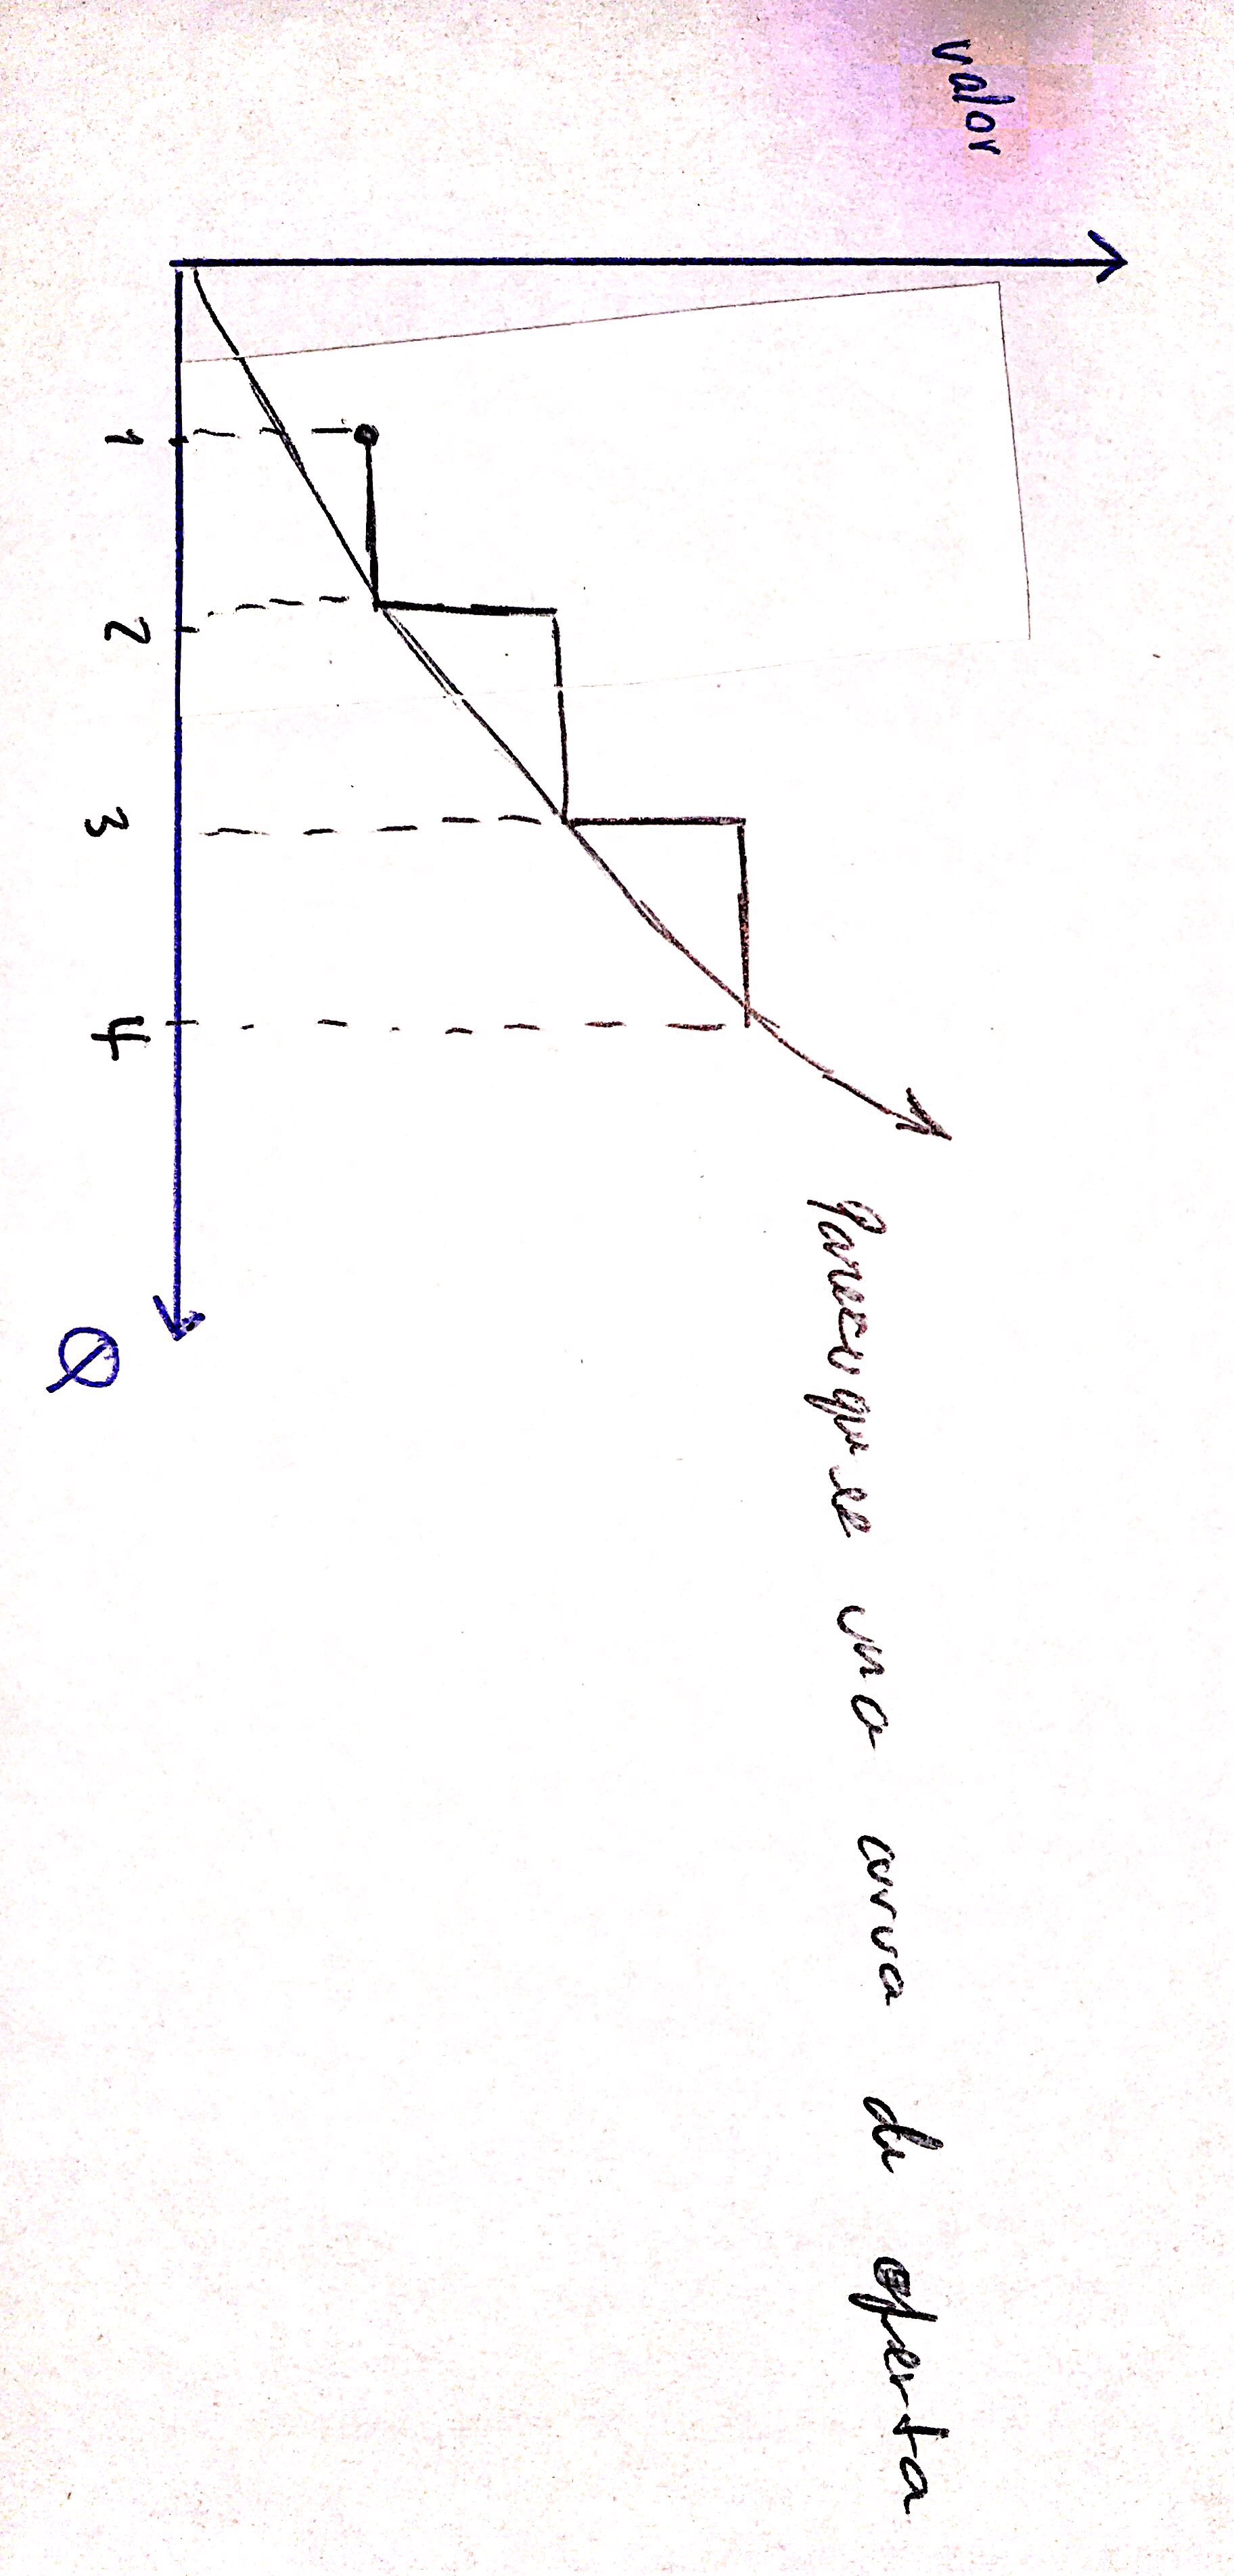
\includegraphics[width=6cm,angle=90]{Classes/Images/2019-07-24-2.jpg}
        \caption{La marginalidad puede interpretarse como una curva de oferta tembién}
        \label{fig2}
    \end{figure}
\end{center}




\section{Oferta y demanda}
Teoría de la utilidad marignal, el principio de utilidad marginal decreciente es \textbf{siempre} decreciente. El reverso de la teoría marginal decreciente coste marginal creciente; la utilida de una unidad más conlleva que todas las unidades van a disminuir de valor.
\begin{center}
    \begin{figure}[htbp]
        \centering
        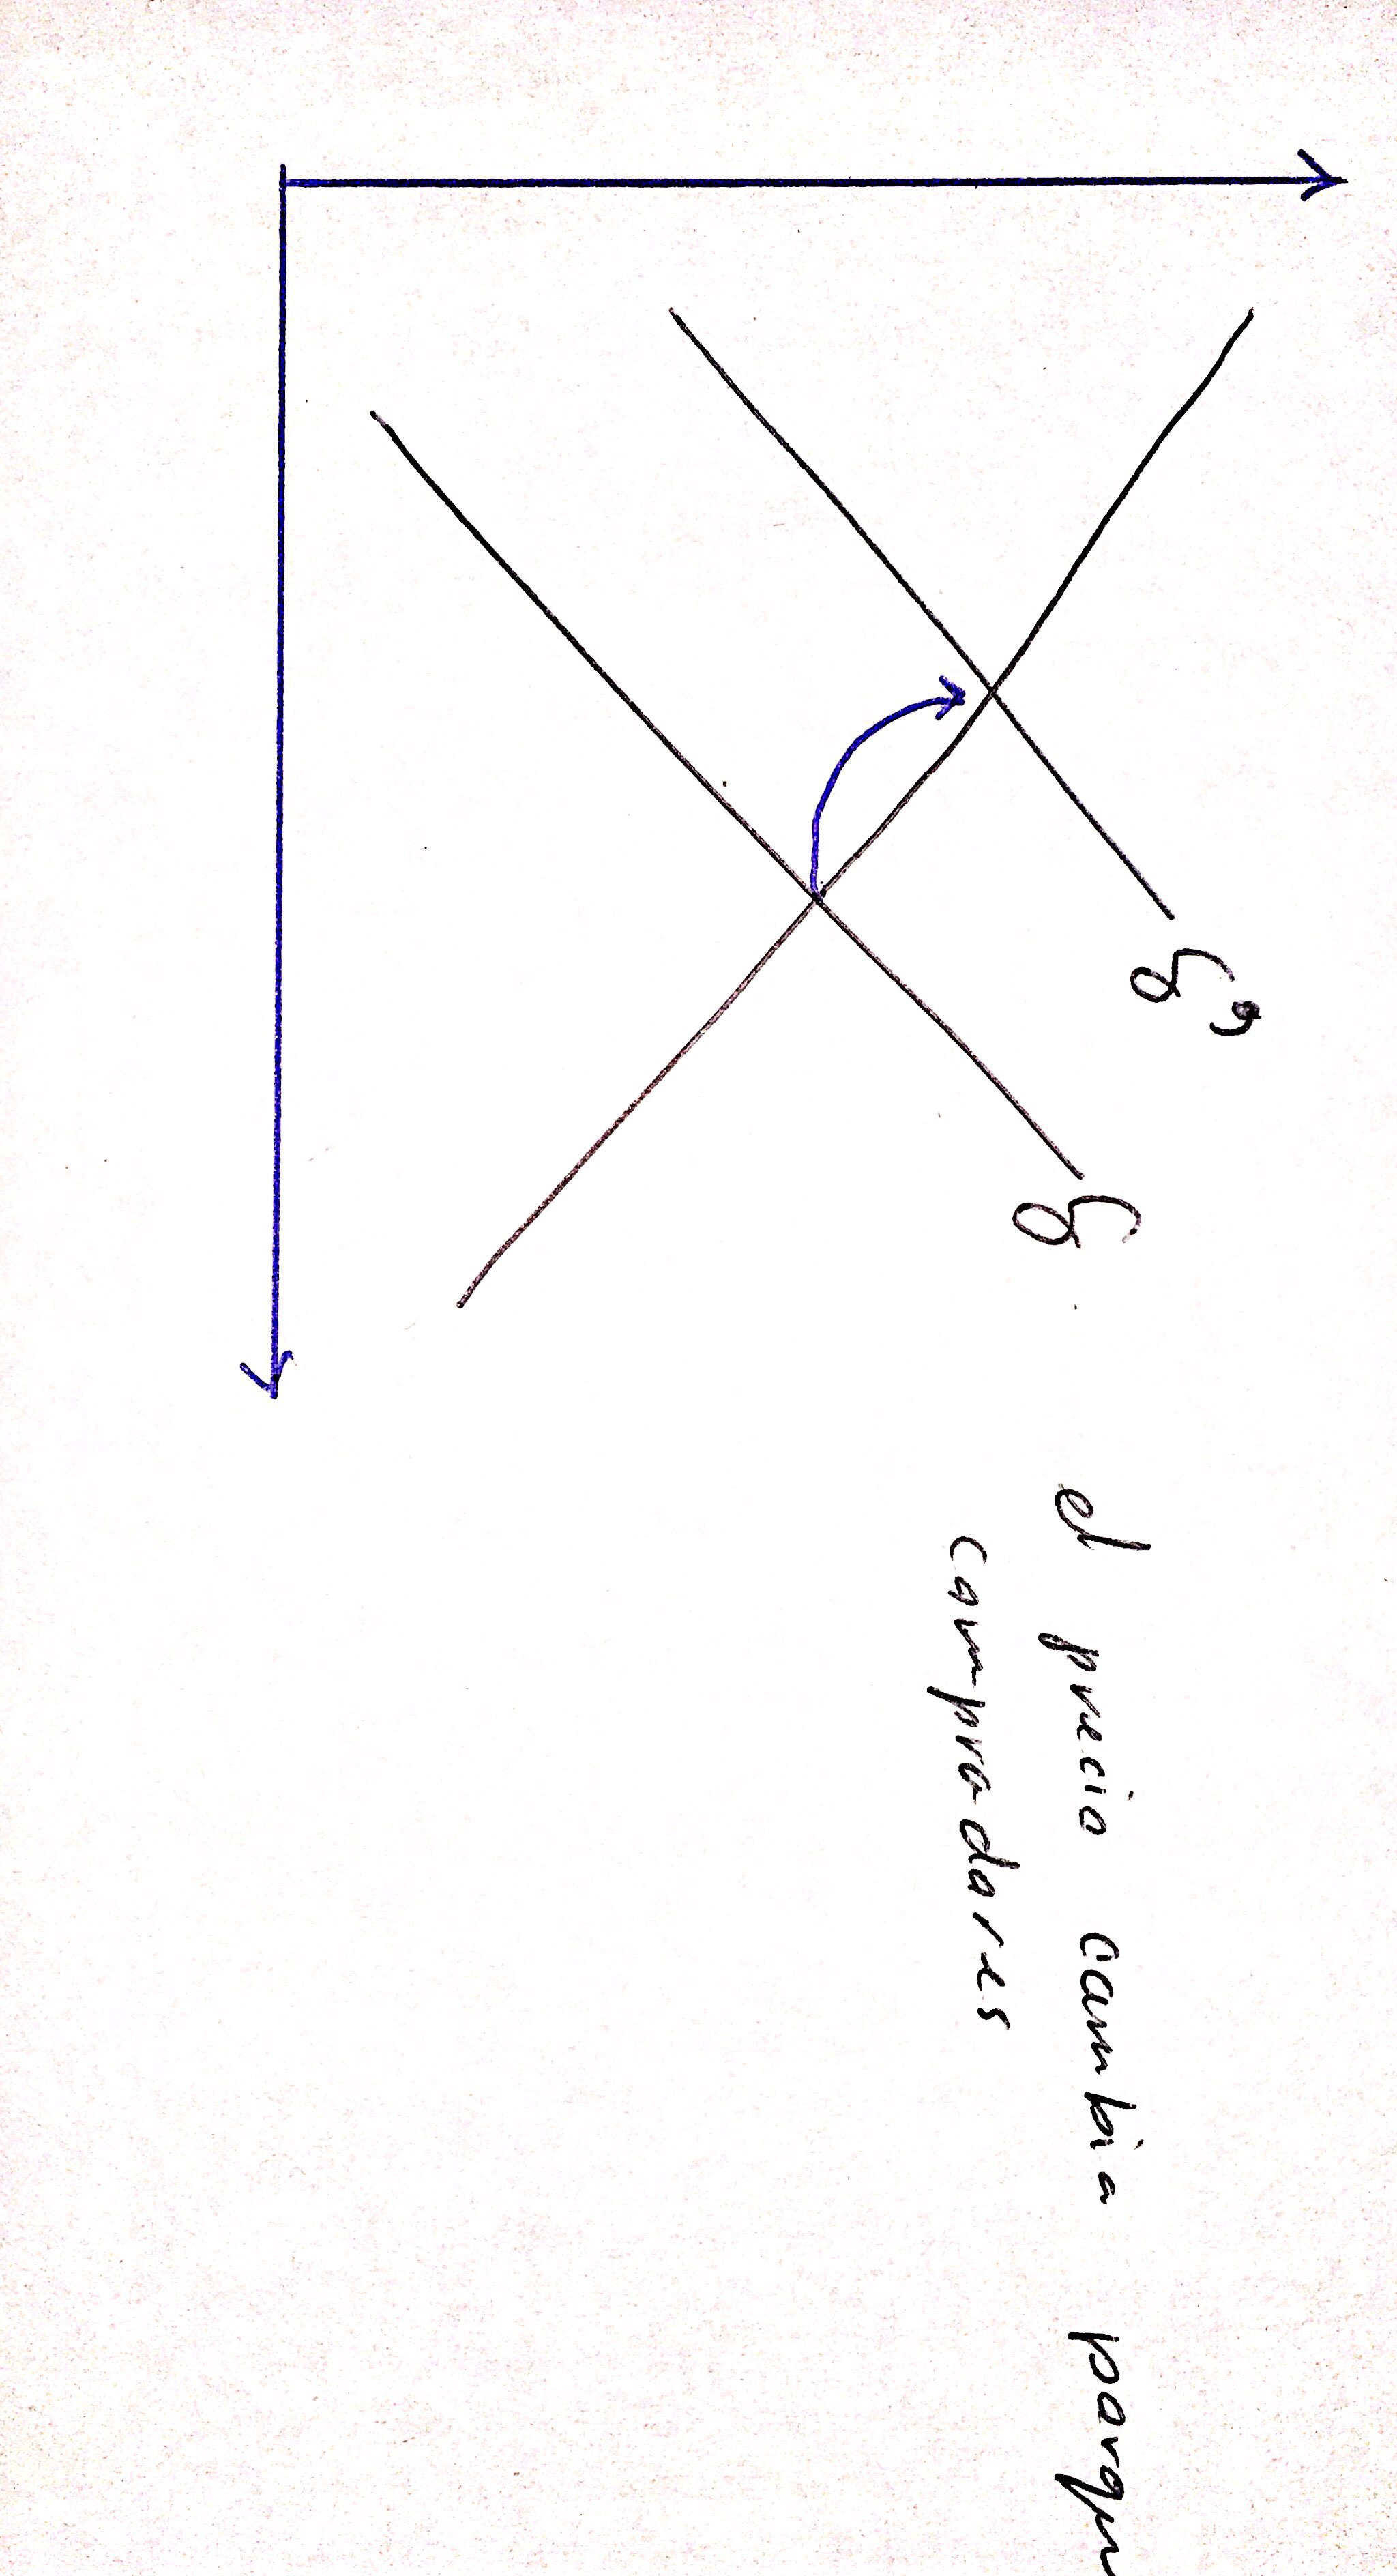
\includegraphics[width=6cm,angle=90]{Classes/Images/2019-07-24-3.jpg}
        \caption{El precio cambia porque los compradores designan una utilidad diferente cada vez y es subjetiva, al igual que los oferentes}
        \label{fig3}
    \end{figure}
\end{center}


\section{Sistema de precios}
Informa de manera indirecta, sobre que producir, con quién producirlo, cuánto producirlo y para quién producirlo. \textbf{Nos preguntamos:} ¿el precio es el determinante o el determinado? El sistema de precio es el determinado. Ejemplo, si un precio sube alguien va a tender a querer meterse a producirlo. El sistema de precios comunica información esencial para que las personas puedan actuar. Es una dinamica de precios que previene la escasez. En general los empresarios persiguen beneficios altos, por eso un empresario le puede parecer mas rentable producir mesas que producir iPhones. Tasa de rentabilidad, qué tanto te vas a tardar en recuperar la inversión. \newline 
Las rentabilidades altas se detruyen con competencia, se tiende a equilibrar, termino 12.27.
% insertar graficas aqui rentabilida.
\begin{center}
\begin{figure}[htbp]
    \centering
    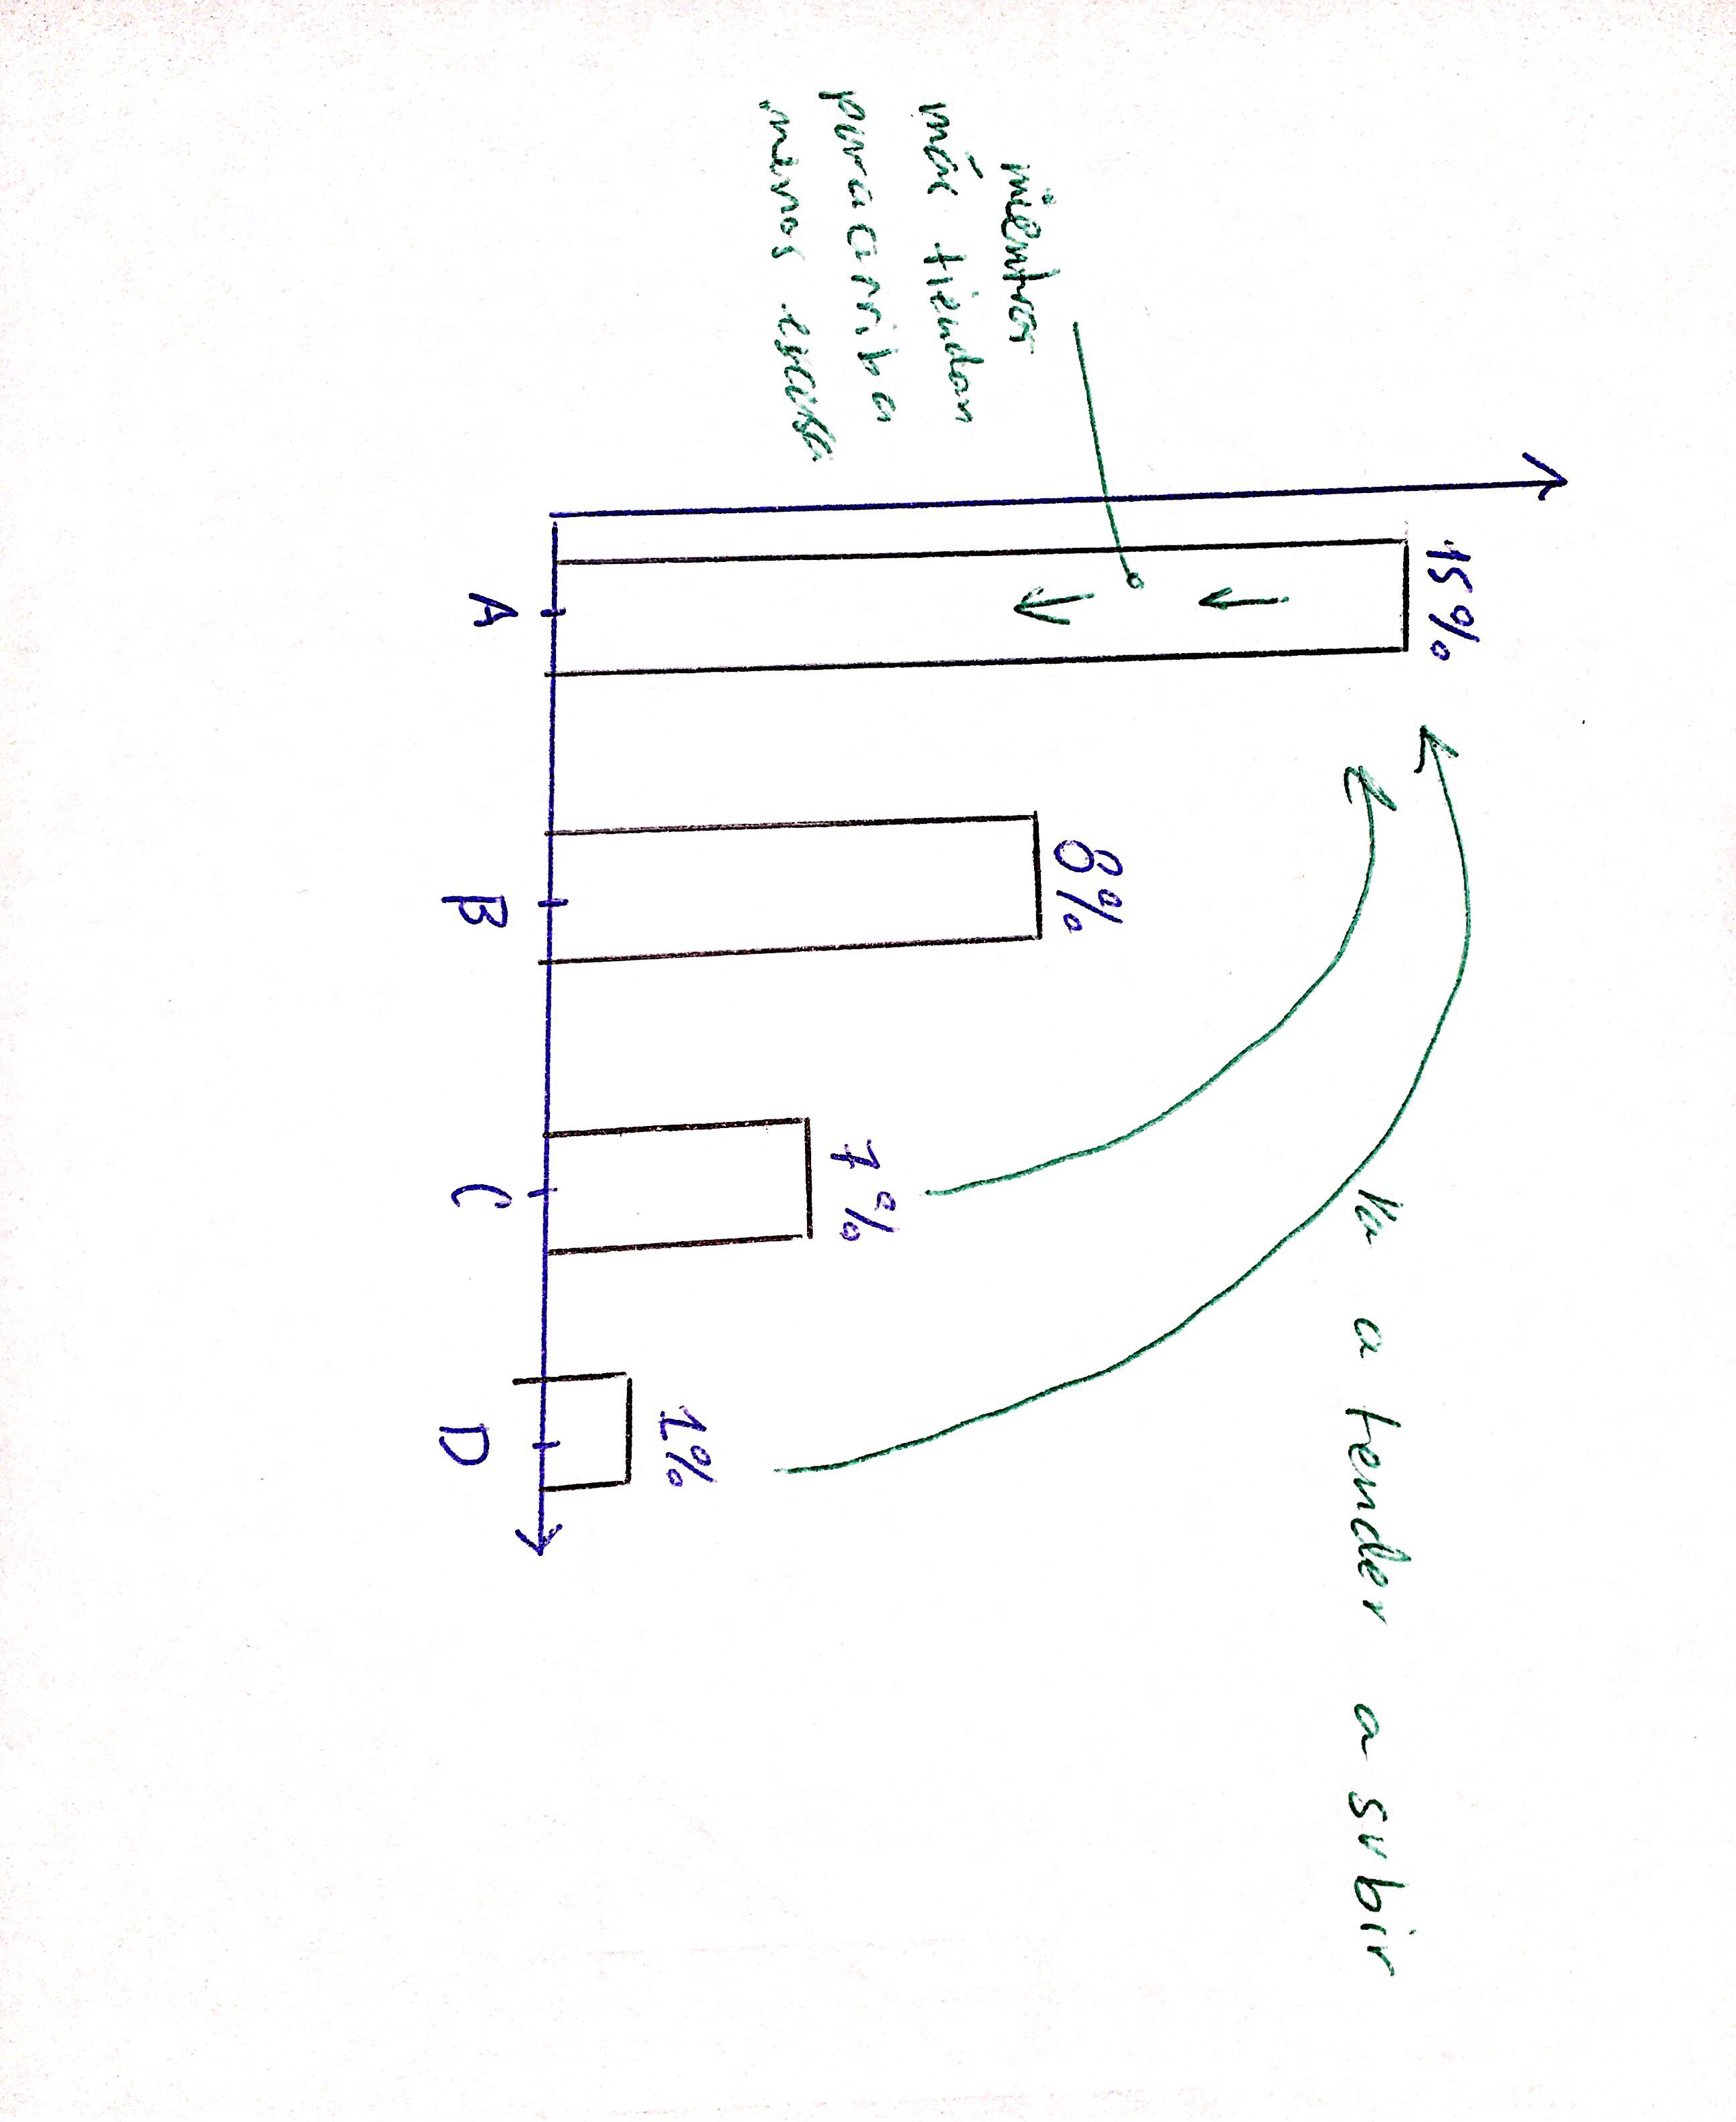
\includegraphics[width=8cm,angle=90]{Classes/Images/2019-07-24-4.jpg}
    \caption{Tiende al equilibrio}
    \label{fig4}
\end{figure}
\end{center}


\section{Subcidios e impuestos}
Si quieres más de algo lo subsidias, si quieres menos de algo pones impuestos. \textbf{Ejemplo: } los ecofiltros regalados, los usaban para masetas, se sobre utiliza. \newline 
\textbf{Ejemplo: } Impuesto a gasolina, se hace caro y la gente lo consume menos. 

\section{Fijación de precios}
Cuando ponen un precio tope se producen faltantes, \textbf{Ejemplo: } el precio de arroz es 3, se presume que es para que toda la gente lo pueda comprar, pero se produce información distorsionada en el sistema de precios y la gente lo empieza a ya no valorarlo. \textbf{Ejemplo: } Venezuela, se controla el harina y el pan, lo que termina produciendo es que todas las panaderías están vacías, si se ponen precios topes se agotan en seguida y nadie le sale rentable producir entonces no se produce. \textbf{Ejemplo: } Los taxis, están a punto de ser erradicado, hay precio minimo de 25Q y ahora lo que ocurre es que los taxis ya no se usan, el precio tope busca controlar la oferta. \textbf{Ejemplo: } El salario mínimo, mientras más pujan el precio del salario minimo para arriba, se aumenta la demanda y se disminuye la oferta, todas las cosas como seguro social, aguinaldo, bono 14, y el salario mínimo termina siendo carísimo. 

\section{Noticia}
Quiz el lunes de la lectura, resumir y analizar la noticia en 5 minutos. 



\chapter{2019-07-29} 
\section{Espacio marítimo y espacio aéreo}
El estado comprende los espacios marítimos siguientes:
\begin{enumerate}
    \item Mar territorial: En Guatemala son 12 millas náuticas, \emph{\textbf{(Paréntesis:}La milla terrestre no es igual a la milla nautica aprx. 0.8km = 1 milla náutica)}
    \item Aguas interiores
    \item Zona económica exclusiva: 200 millas náuticas desde la costa
    \item Zona contigua: 24 desde la costa
    \item Plataforma continental \newline 
    --------------------------------------------
    \item Alta Mar: No forma parte del territorio de un estado. Comprende las partes del mar no incluidas en la zona económica exclusiva. Hay plena libertad de todo.
    \item La zona: No forma parte del territorio de un estado. 
\end{enumerate}

\section{Espacio marítimo}
\textbf{Convención sobre el derecho del mar}: es una convención sobre el derecho del mar, se establece todo como qué medidas cuánto, las medidas del mar territorial. \newline 

\subsection{Derechos el estado Ribeño}
\begin{center}
\begin{tabular}{ | c | c | }
\hline
 Todos los que implique el ejercicio de su soberanía & Por ejemplo: Regular navegación, pesca, investigación  \\
\hline
 Derechos de otros estados & NINGUNO \\  
 \hline
\end{tabular}
\end{center}

\subsection{Zona contigua}
\begin{itemize}
    \item Zona de mar adyacente al mar territorial hasta una distancia de 24 millas marinas contadas desde la líneas de base a partir de las cuales de mide el mar territorial.
    \item \textbf{Derechos del estado}: tomar medidas de fiscalización para prevenir las infracciones aduaneras, fiscales, de inmigración, o cuestiones sanitarias:
    \item \textbf{\emph{Ejemplo:}} Si un barco no identificado se va acercando a la costa y es un potencial peligro al estado no es considerado un paso inocente y se necesita solicitar permiso al estado.
\end{itemize}

\subsection{Derechos de los otros estados}
Derechos de paso inocente:
\begin{itemize}
    \item Se permite pasar simplemente, el barco del aborto por ejemplo no era un paso inocente.
    \item Los cruceros estarían cruzando en la zona contigua, si quiere entrar al mar territorial se necesita pedir permiso al estado.
    \item \textbf{\emph{Definición} :Son pasos que alteran la seguridad de alguna manera en el estado.}
\end{itemize}

\subsection{Zona Económica exclusiva}
\begin{itemize}
    \item 
\end{itemize}

\subsection{Derechos del estado ribereño}
\begin{itemize}
    \item Tiene derechos de soberanía para fines de exploración y explotación, conservación y administración de los recursos naturales vivos y no vivos del lecho y el subsuelo del mar.
    \item Se puede hacer islas en la zona económica exclusiva.
\end{itemize}

\subsection{Borde exteriores de la plataforma continental}
\textbf{\emph{Definición} :Es el lecho de el subsuelo que se encuentra de bajo del suelo del mar, se pueden tener cables, se pueden hacer perforaciones siempre con el consentimiento del estado, fondos marínos y oceanos y su subsuelo fuera de los límites de la jurisdicción nacional.}\newline 
\textbf{\emph{Ejemplo:}} Brooklin 99


\section{Espacio aéreo}
\textbf{\emph{Definición} : el espacio que existe entre la atmósfera y el territorio de un estado} \newline 
Es esencial por:
\begin{itemize}
    \item Mantenimiento de seguridad y defensa del estado
    \item Transporte aéreo
\end{itemize}

\subsection{Tipos de espacio aéreo}
\begin{itemize}
    \item Controlado: aquel espacio donde una torre de control por herramientas como radar se establece un espacio aéreo Controlado
    \item No controlado: \textbf{\emph{Ejemplo:}} torre de control de la aurora y torre de control en peten, pero cuando se fumiga con aviones en fincas solo se avisa cuando se usa el avion para comunicar que uno va a estar en el aire.
    \item Espacio aéreo de uso especial: Con propósitos mas que todo militares, es como un territorio que usa el militar para prácticas de soldados por ejemplo.
    \item Derechos sobre el espacio aéreo: qué se puede hacer.
    \item En cuanto a una línea recta no hay, simplemente se establecieron ciertos criterios.
    \item Libertades del aire: 8 libertades principales, los derechos que tiene un estado.
    \item Se clasifican en libertades técnicas y libertades comerciales.
\end{itemize}

\subsection{Derechos de espacio aereo}
\begin{enumerate}
    \item Libertad de pasar sin aterrizar.
    \item Falla técnica, tiene derecho a aterrizar por emergencias. \textbf{\emph{(Ejemplo:una señora se sentía mal en un vuelo de EEUU a Guatemala, se tuvo que seguir un protocolo que atrasó 1:30h y media.)}} Referente a vuelos internos.
    \item Libertades comerciales: desembarque \textbf{\emph{(Ejemplo: pasajeros, correo y carga tomados en el territorio del país cuya nacionalidad posee la aeronave.)}} Involucra lucro. Referente a vuelos internos.
    \item Embarcar, es una libertad comercial de embarque. Involucra lucro.
    \item Poder embarcar y desembarcar en cuanto matrículas de estados diferentes.
\end{enumerate}

\subsection{Espacios ultra-terrestres}
\begin{itemize}
    \item Son espacios como la luna y otros cuerpos celestes
    \item Regula en cuanto a lo que el ser humano pueda mandar a la orbita, ya que despues de cierto tiempo se convierte en desechos
    \item Los cuerpos celestes son patrimonio común.
    \item Regulación constitucional:
    \begin{itemize}
        \item Art. 121 literal b
        \item Art 142 literal a 
    \end{itemize} 
    \item Dirección general de aeronáutica civil
    \begin{itemize}
        \item Regulada en el decreto número 93-2000
        \item Art 3
        \item Art 7 literal a
        \item Art 66
    \end{itemize}
    \item Los derechos de la política de cielos abiertos: reconocer el embarque y desembarque de naves de diferente nacionalidad.
\end{itemize}

\subsection{En Guatemala}
\begin{itemize}
    \item Regulación de drones:
    \begin{itemize}
        \item Aeronaves no tripuladas
        \item Necesidad de registro
    \end{itemize}
    \item Globos aerostáticas:
    \begin{itemize}
        \item RAC 31
    \end{itemize}
    \item Vuelos en parapente y ala delta:
    \begin{itemize}
        \item RAC 103
    \end{itemize}
\end{itemize}

\subsection{Tarea}
\textbf{}   


\chapter{2019-08-31}
\section{Elementos posteriores del estado}

\subsection{El poder}
\begin{itemize}
    \item El poder: En la antigüedad, se necesitaba el estado, la gente buscaba el poder en gobernantes que consideraban dignos de gobernar. 
    \begin{itemize}
        \item El estado \textbf{\emph{Caso ``Juan Sitierra": Era un gobernante }}, se buscaba orden. no puede existir sin poder, no puede existir sin llegar a su fin tempora. y no se puede llegar al fin sin poder. El estado impone el orden a través del poder.
        \item Orden:Se considera mucho el orden, tiene que haber orden.
        \item Poder (autoridad): poder no es absoluto
    \end{itemize}


    \item Características del poder:
    \begin{enumerate}
        \item No es absoluto, \textbf{\emph{Definición: Absoluto es un poder sin límites, como Luis XIV}}, lo que más regula el comportamiento de los gobernantes es la \textbf{Constitución}, hoy en día se tiene límites.
        
        \item Supremo o soberano; es supremo pero no absoluto, el poder es el máximo poder de un territorio y todo lo que conlleva su territorio, es supremo y soberano, el poder esta por encima de todos los demás poderes.
        
        \item Poder de derecho = ordenamiento jurídico; \textbf{\emph{Caso ``Quiché": El mismo pueblo indígena en Nebaj se da el caso de derecho indígena. Es más una ausencia de la autoridad.}}, significa que está determinado por un ordenamiento jurídico.
        
        \item Poder de dominación = Coacción; \textbf{\emph{Definición:  El estado puede ejercer su poder por coacción, o por fuerza.}}
    \end{enumerate}

    
    \item Tareas del poder
    \begin{center}
    \begin{tabular}{ | p{6cm} | p{8cm} | } 
     \hline
    Gobernar & Administrar \\
    \hline
    Dirección de los ciudadanos & Organización de la función administrativa \\
    \hline
    Se gobierna a persona & Se administran cosas \\ 
    \hline
    Mandatos & Satisfacción de necesidades COLECTIVAS \textbf{\emph{(Ejemplo: Carreteras, servicios, públicos)}} \\
     \hline
    \end{tabular}
    \end{center}

    Administrar \textbf{\emph{Definición: se refiere mas que todo a prestar servicios públicos}} \newline 
    Gobierno \textbf{\emph{Definición: Formular mandatos para la conservación dek estado y para el logro de sus fines.}}

    
    \item Soberanía:
    \begin{itemize}
        \item \textbf{Nos preguntamos:} ¿Cómo definirían la soberanía? \emph{(\textbf{Respuesta}:Es el poder supremo. y soberano es })
        \item Art. 141 Constitución; La subordinación entre las ramas del estado es prohibida \textbf{\emph{Caso ``Baldeti y la corrupción": Daba dinero a diputados para aprobar ciertas leyes.}}
        \item \emph{\textbf{(Paréntesis:}Las ramas del estado, ejecutivo, legislativo y judicial. El Art. 141 frena a los tres poderes entre sí)}
        \item El sujeto de la soberanía es el estado: 
        \begin{itemize}
            \item Doctrinas de la soberanía Absolutista, popular y soberanía nacional.
        \end{itemize}
    \end{itemize}

    
    \item ¿Cómo se debe ejercer el poder público en Guatemala?
    \begin{itemize}
        \item Art. 152 Poder público: El poder que ejercen las autoridades públicos del estado. Como se transmite la soberanía a alguien para poder ejercer el obierno y administración.
        \item Art. 153 Imperio de la ley: la ley se extiende a todos sean extranjeros o nacionales se aplica la ley Guatemalteca.
        \item Art. 154  Función pública: \textbf{\emph{(Ejemplo: Los juramentos de jurar defender la constitución)}}
        \item Art. 155 Responsabilidad por infracción a la ley: \textbf{\emph{(Ejemplo: si un funcionario comete un delito, por el hecho de ser funcionario se duplica la pena por el delito.)}}
        \item Art. 156 No obligatoriedad de órdenes ilegales: Ningún funcionario es obligado a obedecer algo que no es legal.
    \end{itemize}

    
    \item El fin es el Bien común: 
    \begin{itemize}
        \item Fin de un estado definido en la Constitución: Art. 1 de la constitución. 
        \item Art.1 Constitución de Guatemala
        \item ¿Cómo definirían el Bien Común? \textbf{\emph{Definición: Bien común, es el conjunto de condiciones sociales, económicas, culturales, morales y espirituales para desarrollarnos}}
        \item \emph{\textbf{(Paréntesis:}En el preámbulo de la constitución de Guatemala, se establece que se va a preferir por default el bien común sobre el bien individual.)}
    \end{itemize}

    \item \emph{\textbf{(Paréntesis:}Razón del estado, teoría que sostiene que el individuo está a la disposición del estado. La teoría de derecho natural, Guatemala sostiene esta teoría ya que el estado esta al servicio de el individuo, es al revéz que la razón del estado.)} \emph{\textbf{(Paréntesis:}Libertad de credo la asegura la constitución pero así como no hay idioma oficial la constitución está escrita en español, asi mismo pasa con la religión Art. 36 Libertad de religión)}
    
    \item Orden jurídico
    \begin{itemize}
        \item \textbf{Nos preguntamos:} ¿Qué entienden por orden jurídico? Ultimo elemento posterior es el orden jurídico, el estado esta sujeto a normas internas y externas.
        \item Estado con otros Estados = Normas de Derechos Internacionales
        \item Estado con Gobernados = Normas Jurídicas Internas
    \end{itemize}

    
    \item La necesidad del derecho en un estado.
    \begin{itemize}
        \item No se concibe al Estado sin Derecho ni al  Derecho sin Estado. 
        \item “Un Estado sin poder soberano es inconcebible, y un Estado con poder que no esté limitado por el Derecho, no es Estado sino fenómeno de fuerza”
    \end{itemize} 

    \item \emph{\textbf{(Paréntesis:}El derecho y el estado según mucho sautores son lo mismo pero en este curso se tratarán como diferentes por la razón que es un ordenamiento jurídico.)}
\end{itemize}

\subsection{Noticia: Conflicto Mexico-Guatemala}
\begin{itemize}
    \item Conflictos acerca de tala de arboles en Petén.
    \item El bombardeo de los barcos.
    \item México corta lazos diplomáticos.
    \item Se resuelve el conflicto.
    \item \emph{\textbf{(Paréntesis:}Relacionar con la soberanía Guatemalteca.)}
\end{itemize}

\begin{itemize}
    \item Sealand
\end{itemize}




\chapter{}
\section{Diferencias entre UX/UI}
\subsection{UX}
\begin{enumerate}
    \item User Research
    \item User Personas 
    \item User flow diagrams
    \item Usability testing
    \item A/B testing 
    \item Measurements
\end{enumerate}
%%%%%%%%%%%%%%%%%%%%%%%%%%%%%%%%%%%%%%%%%%%%%%%%%%%%%%%%%%%%%%%%%%%%%%%%%%%%%%%%%%%%%%%%%%%%%%%%
\subsection{UI}
\begin{enumerate}
    \item Colors 
    \item Typography
    \item Color constrast 
    \item Accesibility 
    \item High fidelity prototypes 
    \item Overall look and feel
\end{enumerate}
\emph{\textbf{(Paréntesis:}Entrarían html y css, si tenés tiempo.\textbf{)}}
%%%%%%%%%%%%%%%%%%%%%%%%%%%%%%%%%%%%%%%%%%%%%%%%%%%%%%%%%%%%%%%%%%%%%%%%%%%%%%%%%%%%%%%%%%%%%%%%
\section{Proceso}
Hay varios métodos pero el más conocido y usado es el siguiente:
\begin{enumerate}
    \item Research: una de las partes más importantes para determinar qué podemos hacer, evaluar cómo opera la competencia, 
    \item Sketched: Los bocetos, cuando uno hace el research se le ocurren ideas, estos son machotes, son una lluvia de ideas que se utiliza para descartar ideas, normal mente son a mano.
    \item Wireframe: es una versión más refinada de los sketches, en los wireframes no se emite la versión terminada pero tenes que pensar más en lo realístico al producto final, vas a tomar en cuenta el dispositivo el cual tu app va a correrse.
    \item Mockups: Es la versión terminada de los mockups, se define casi que nada, esta es la version \underline{final} del producto.
    \item Prototyping: el prototipo es agarrar todos los mockups que tenemos y prototiparlo.
    \item Testing: esto es para medir qué tan buenos resultados están los resultados de los mockups, si no están al gusto del project manajer se repite la iteración.
\end{enumerate}
%%%%%%%%%%%%%%%%%%%%%%%%%%%%%%%%%%%%%%%%%%%%%%%%%%%%%%%%%%%%%%%%%%%%%%%%%%%%%%%%%%%%%%%%%%%%%%%%
\section{Aplicación a diseño en la vida real}
A continuación 
\begin{enumerate}
    \item Resource: qué tanto personal contamos con.
    \item Requerimientos: definen el ``qué hacer'', son los requisitos básicos que tienen que tener el producto, a veces uno propone algo mejor pero hay que respetar que tenemos esos requisitos.
    \item Deadline: uno empieza a economizar y ver si se puede saltar pasos en el proceso, probablemente saltar de sketches a mockups, por ejemplo.
    \item Availability: quiénes van a estar disponible, hay feriados en la iteración, alguien va a estar de vacaciones.
    \item Product type: qué estoy tratando de lograr desde lo que estoy diseñando, \emph{\textbf{Ejemplo:}un botón, una pagina de checkout}
\end{enumerate}
%%%%%%%%%%%%%%%%%%%%%%%%%%%%%%%%%%%%%%%%%%%%%%%%%%%%%%%%%%%%%%%%%%%%%%%%%%%%%%%%%%%%%%%%%%%%%%%%
\section{Buenos y malos ejemplos de UX}
\begin{itemize}
    \item Claridad en el producto, los parqueos y las señales de parqueo por ejemplo.
    \item \emph{\textbf{Ejemplo:} Formulario, la gran lista de países.}
    \item \emph{\textbf{Ejemplo:} Por ejemplo la eliminación de mensajes de whatsapp}
\end{itemize}
%%%%%%%%%%%%%%%%%%%%%%%%%%%%%%%%%%%%%%%%%%%%%%%%%%%%%%%%%%%%%%%%%%%%%%%%%%%%%%%%%%%%%%%%%%%%%%%%
\section{Trabajando con Project manajers y developers}
\textbf{Nos preguntamos:} ¿Cómo trabajo con tantas personas sin hacer un gran problema?
\begin{enumerate}
    \item Tener un timeline
    \item Definir prioridades
    \item Trabajar en equipo
    \item Mantener a todo el equipo al tanto en todo momento
\end{enumerate}
Teninendo un timeline y prioridades se puede evitar conflicto, \textbf{Nos preguntamos:} ¿qué pasa cuando dos productos prioritarios? \emph{\textbf{La respuesta a esta pregunta es: }tenemos que priorizar sólo uno de primero, normalmente se hace esto entre PM y usualmente solo se le informa al developer que deje de hacer lo que está haciendo y que se trabaje en lo que está prioridades}
%%%%%%%%%%%%%%%%%%%%%%%%%%%%%%%%%%%%%%%%%%%%%%%%%%%%%%%%%%%%%%%%%%%%%%%%%%%%%%%%%%%%%%%%%%%%%%%%
\section{Herramientas}
\begin{enumerate}
    \item Figma: es una herramienta multi-plataforma, es administrador de versiones, tiene versión web, tiene plugins que ayudan a diseñar más rápido.
    \item Sketch: sólo MAC, plug-ins, smart layouts, es pagado.
    \item Adobe XD, MAC/Windows, plugins, es gratis.
\end{enumerate}
%%%%%%%%%%%%%%%%%%%%%%%%%%%%%%%%%%%%%%%%%%%%%%%%%%%%%%%%%%%%%%%%%%%%%%%%%%%%%%%%%%%%%%%%%%%%%%%%
\section{\textbf{Nos preguntamos:} ¿Se puede programar y diseñar?}
\emph{\textbf{La respuesta a esta pregunta es: }Sí, es aún mejor tener los conocimientos para ser más ágiles a la hora de tener conflictos, tener en cuenta qué se puede hacer y qué no, entre más sepa de diseño mejor, mientras más sepa de programación mejor.}
%%%%%%%%%%%%%%%%%%%%%%%%%%%%%%%%%%%%%%%%%%%%%%%%%%%%%%%%%%%%%%%%%%%%%%%%%%%%%%%%%%%%%%%%%%%%%%%%
\section{Ventajas de diseñar y programar}
\begin{enumerate}
    \item Diseñar teniendo en cuenta la parte técnica.
    \item No vamos a diseñar cosas complejas ni para los usuarios ni para los devs.
    \item Diseño teniendo en cuenta la implementación.
    \item Hablar el lenguaje de los desarrolladores.
    \item Asegurarse que el diseño hecho quede igual una vez implementado.
    \item Ofrecer ayuda.
\end{enumerate}
%%%%%%%%%%%%%%%%%%%%%%%%%%%%%%%%%%%%%%%%%%%%%%%%%%%%%%%%%%%%%%%%%%%%%%%%%%%%%%%%%%%%%%%%%%%%%%%%
\section{\textbf{Nos preguntamos:} ¿Qué debemos hacer para programar?}
\begin{enumerate}
    \item HTML: estructura
    \item CSS: estilo
    \item JavaScript (un poquito solamente lo necesario), hay diseñadores que le tienen miedo a JavaScript.
    \item Responsive device
\end{enumerate}
%%%%%%%%%%%%%%%%%%%%%%%%%%%%%%%%%%%%%%%%%%%%%%%%%%%%%%%%%%%%%%%%%%%%%%%%%%%%%%%%%%%%%%%%%%%%%%%%
\section{Tres pilares de csss}
\begin{enumerate}
    \item Herencia: los hijos heredan los estilos de los padres, para ahorrar código.
    \item Especifidad: hay elementos en nuestro código son especificamente modificados para esos elementos selectos para que no hereden las características estipuladas si no que se comporten de una manera diferente.
    \item Cascada: dos clases que se llaman lo mismo y la que se va a aplicar va a ser la última. 
\end{enumerate}
Ver: EDteam.com 
%%%%%%%%%%%%%%%%%%%%%%%%%%%%%%%%%%%%%%%%%%%%%%%%%%%%%%%%%%%%%%%%%%%%%%%%%%%%%%%%%%%%%%%%%%%%%%%%
\section{\textbf{Nos preguntamos:} ¿Qué es responsive Web Design?}
\begin{enumerate}
    \item Es básicamente condicionales, tener en cuenta qué dispositivos estarán usando la aplicación.
    \item Una condicional que no afecte nada más que defina el comportamiento en diferentes dispositivos para acomodar bien todo según el dispositivo esto es para responsive, la condicional ``media query''.
\end{enumerate}
%%%%%%%%%%%%%%%%%%%%%%%%%%%%%%%%%%%%%%%%%%%%%%%%%%%%%%%%%%%%%%%%%%%%%%%%%%%%%%%%%%%%%%%%%%%%%%%%
\section{Resources}
\subsection{U-en-línea}
\begin{enumerate}
    \item Product design, udacity
    \item design.io
    \item learnux.io 
    \item platzi.com 
    \item ed.team 
    \item codigofacilito.com 
    \item udemy.com 
    \item udacity.com 
    \item youtube.com 
\end{enumerate}
\subsection{Inspiración}
\begin{enumerate}
    \item dribble.com 
    \item behance.net 
    \item uplabs.com 
    \item material.io 
    \item pttrns.com 
\end{enumerate}


\chapter{}
\section{Caracteres del derecho}
\begin{itemize}
    \item \textbf{Nos preguntamos:} ¿por qué el derecho es un fenómeno social?
    \begin{itemize}
        \item por que es una obra humana,  es creado por el hombre, dicta el comportamiento para poder vivir en sociedad.
        \item El hombre es el que lo crea, para funcionar tiene que crear normas.
    \end{itemize}
    
    \item \textbf{Nos preguntamos:} ¿por qué el derecho es un fenómeno cultural?
    \begin{itemize}
        \item Si se impusiera una norma que funciona en otro país no implica que vaya funcionar por la razón cultural
    \end{itemize}

    \item \textbf{Nos preguntamos:} ¿por qué el derecho es un fenómeno Histórico?
    \begin{itemize}
        \item Por que el derecho cambia a través del tiempo, cosas que funcionaban en un tiempo y ahora ya no o vise versa.
        \item Se cambia por que en algún momento se consideró importante.
        \item \textbf{Nos preguntamos:} ¿qué evoluciona más rápido la sociedad o el derecho? \emph{(\textbf{Respuesta}:es la sociedad, lo ideal es que el derecho evolucione a la par de la evolución de la sociedad })
        \item Puede cambiar retrocediendo o progresando. \textbf{\emph{(Ejemplo: El derecho involucionó en el caso de Hitler, el ejemplo del voto por ejemplo)}}
        \item \emph{\textbf{(Paréntesis ``Hábeas corpus exhibición personal'':} se puede emitir una solicitud al juez para determinar la legalidad del derecho \textbf{)}}
    \end{itemize}

    \item \textbf{Nos preguntamos:} ¿por qué el derecho es un fenómeno político? Sí por que expresa relaciones con el poder, por ejemplo la coacción.
    
\end{itemize}

\section{Acepciones del derecho}
\begin{itemize}
    \item Problemas de ambigüedad:
    \begin{itemize}
        \item Es confuso, significados diferentes en los que la terminología se refiere a muchas cosas y depende del contexto, \textbf{\emph{(Ejemplo: mora, fruta o multa por retraso a obligaciones, ejemplo la alimentación y la ambigüedad de eso, otro ejemplo ``competente''.)}}
    \end{itemize}

    
    \item Vaguedad:
    \begin{itemize}
        \item Se desconoce el alcance, falta claridad.
    \end{itemize}

    
    \item Emotividad: 
    \begin{itemize}
        \item Tiene una carga emotiva, relacionado con las emociones, \textbf{\emph{(Ejemplo: la justicia)}}
    \end{itemize}

    
    \item Distintas acepciones del ``derecho'':
    \begin{itemize}
        \item Tiene varios significados:
        \begin{enumerate}
            \item Derecho como facultad o derecho subjetivo:
            \begin{itemize}
                \item ``Tengo \underline{\textbf{derecho}} a algo''
            \end{itemize}
            
            \item Derecho como ciencia:
            \begin{itemize}
                \item Se usa científicamente en el área académica, es estudio como una ciencia .
            \end{itemize}
            
            \item El derecho como ideal ético o moral de \underline{\textbf{Justicia}}: 
            \begin{itemize}
                \item Relacionados con lo justo según lo moral o ética, se usa al derecho como lo que ``es justo''.
            \end{itemize}
            
            \item El derecho como la norma:
            \begin{itemize}
                \item Derecho objetivo, es las referencias a las normas escritas.
            \end{itemize}
        \end{enumerate} 
        
        De dónde se deriva:
        \begin{enumerate}
            \item De todo derecho objetivo se derivan los subjetivos.
        \end{enumerate}
        
        En otros lenguajes como el inglés:
        \begin{itemize}
            \item Derecho subjetivo = right 
            \item Derecho objetivo = law
        \end{itemize}

        Tesis de la indefinición: es imposible de definirlo en su totalidad, solo parcialmente. 

        
        \item Derecho subjetivo:
        \begin{itemize}
            \item El derecho subjetivo público:
            \begin{itemize}
                \item Cuando el estado se mete en los derechos. \textbf{\emph{(Ejemplo: subsidios)}}
            \end{itemize}
            
            \item El derecho subjetivo privado:
            \begin{itemize}
                \item Cuando el estado no se mete, por ejemplo cuando se da una cobra venta. Ojo, el estado puede tener un carácter de individuo particular.
            \end{itemize}
            
            
        \end{itemize}
    \end{itemize}
        

    Clases de derecho objetivo:
        \begin{itemize}
            \item El derecho objetivo orientado al derecho natural:
            \begin{itemize}
                \item Orientado a aquello que el humano tiene como intuición de qué es lo bueno, el derecho natural no cambia y permanece constante.
                \item Evolución de el derecho natural:
                \begin{itemize}
                    \item Época antigua $\rightarrow$ Naturaleza del hombre
                    \item Época cristiana $\rightarrow$ Dios (autoridad suprema)
                    \item Época moderna $\rightarrow$ El D. natural se origina en la razón.
                    \item Renacimiento del derecho natural $\rightarrow$ Reconocimiento de derechos humanos
                \end{itemize}

                
                \item Diferencias: \newline 
                \begin{tabular}{ | p{5cm} | p{5cm} | } 
                 \hline
                \textbf{El derecho natural} & \textbf{El derecho positivo} \\
                Inherente al hombre & Se crea autoridad competente \\ 
                Inmutable & Mutable \\ 
                Universal & Es reflejo de la cultura \\ 
                Justo & No siempre es justo \\ 
                Incoersible & Coercible \\ 
                 \hline
                \end{tabular}
                
            \end{itemize}

            \item El derecho objetivo orientado al derecho positivo:
            \begin{itemize}
                \item No es creado por el hombre, el derecho positivo no es igual en todos los tiempos.
            \end{itemize}

            
            \item Iuspositivismo:
            \begin{itemize}
                \item Admite la distinción del derecho natural y el positivismo.
            \end{itemize}
        \end{itemize}
        
        \item Clasificación del derecho positivo:
        \begin{itemize}
            \item Por su grado de efectividad:
            \begin{enumerate}
                \item Vigente
                \item No vigente:
                \begin{itemize}
                    \item Actual, no efectiva ahorita, no van a limitar nada innecesario (ley de orden público, \textbf{\emph{(Ejemplo: el asesinato de militares causó una limitación en los derechos de la constitución, estado de sitio)}})
                    \item Histórico: derogado 
                \end{itemize}
            \end{enumerate}
            
            \item Por su forma de manifestarse:
            \begin{itemize}
                \item Escrito: plasmado en documentos.
                \item No escrito: costumbre (derecho consuetudinario) \textbf{\emph{(Ejemplo: derecho indígena)}}
            \end{itemize}

            
            \item Por materia que regula:
            \begin{itemize}
                \item Derecho público: interviene el estado con poder soberano o como institución pública. 
                \item Derecho privado: entre el particulares. 
                \item \textbf{Nos preguntamos:} ¿puede intervenir el estado en una relación de derecho privado? \emph{\textbf{La respuesta a esta esta pregunta es: }...}
            \end{itemize}
        \end{itemize} 







    \end{itemize}
    

\section{Teorías que explican la división del derecho en público y privado}
\begin{itemize}
\item Teoría del interés:
\begin{itemize}
    \item Público: interes colectivo
    \item Privado: interes particular 
\end{itemize}

\item Teoría del organo:
\begin{itemize}
    \item Público: estado interviene 
    \item Privado: estado no interviene
\end{itemize}

\item Teoría del interés:
\begin{itemize}
    \item Privado: relaciones de coordinación, es de peers.
    \item Público: relaciones de subordinación o supraordinación
\end{itemize}
\end{itemize}

\section{Derecho público}
\textbf{Irrenunciable e innomidicable:} No nos queda otra que obedecer, no es renunciable ni modificable.
\begin{itemize}
    \item Derecho Constitucional (Derechos fundamentales): constitución 
    \item Derecho Fiscal (SAT): impuestos
    \item Derecho Administrativo (Municipalidades): sacar pasaporte, licencia, permisos de construcción etc.
    \item Derecho Penal (Delitos): sansiones y coacción.
    \item Derecho Procesal (Procesos judiciales): normas establecidas para procesos legales.
    \item Derecho Internacional Público (Tratados y convenios internacionales TLC): CONVEMAR, TLC's, etc.
    \item Derecho laboral (relación con empleados): \textbf{es un área gris} puede pactarse con el patrono y el empleado qué suma de dinero hay que pagarle siempre y cuando no sea menos del salario mínimo, tengo libertad de pagarle cualquier suma arriba del mínimo. Es entre particulares pero por la constante intervención del estado es un derecho público. Proteccionismo de parte del estado al trabajador. \newline \textbf{\emph{(Ejemplo: fallecimiento de trabajador con la esposa conflicto con los Q1,000)}}, \textbf{\emph{(Ejemplo: premisa que todos los trabajadores pueden joder a los patronos sin evidencia.)}}, \textbf{\emph{(Ejemplo: Ventana económica, todo lo adicional que le da el patrono al trabajador hace mas caro cualquier cosa, puede exigir 30\% más en su indemnización.)}}, \textbf{en GT se considera derecho público}. \textbf{Es frecuente el abuso del trabajador al patrono}.
\end{itemize}

\section{Derecho privado}
\textbf{Renunciable y modificable:} sí se puede renunciar.
\begin{itemize}
    \item Derecho Civil (Contratos): contratos. Vendo la casa por que no la uso no por fin de lucro. \textbf{\emph{(Ejemplo: viaje con cosas que parecen ser de comercio pero son civil.)}}
    \item Derecho Mercantil (Fin de lucro):tienen fin de lucro, ejemplo: títulos de crédito, sociedades. 
    \item Derecho Internacional Privado (Legislación aplicable): casarse en otro país, con una persona extranjera, cambio de nombre, cambio de nacionalidad.
\end{itemize}



\chapter{}
\section{Levantar Redis}
%%%%%%%%%%%%%%%%%%%%%%%%%%%%%%%%%%%%%%%%%%%%%%%%%%%%%%%%%%%%%%%%%%%%%%%%%%%%%%%%%%%%%%%%%%%%%%%%

\section{JavaScript}
\begin{enumerate}
    \item JavaScript, se puede hacer todo con JS.
    \item Ventajas: comunidad demasiado grande.
    \item Vanilla JavaScript, es plain, Angular $\neq$ JavaScript. 
\end{enumerate}
%%%%%%%%%%%%%%%%%%%%%%%%%%%%%%%%%%%%%%%%%%%%%%%%%%%%%%%%%%%%%%%%%%%%%%%%%%%%%%%%%%%%%%%%%%%%%%%%
\section{Traducción de Python $\Rightarrow$ JavaScript.}
\begin{center}
\begin{tabular}{ | p{5cm} | p{5cm} | }
 \hline
Python & JavaScript \\
 \hline
def(...): & function(...){...}\\ 
if ...: & if(...){...}\\ 
while ...: & while (...){...}\\ 

\end{tabular}
\end{center}

%%%%%%%%%%%%%%%%%%%%%%%%%%%%%%%%%%%%%%%%%%%%%%%%%%%%%%%%%%%%%%%%%%%%%%%%%%%%%%%%%%%%%%%%%%%%%%%%
\section{Homework}
\begin{enumerate}
    \item ECMA Script 
    \item Weakly typed / Strongly typed
    \item Asynchronous of JavaScript - Call Stack
    \item Event loop 
    \item \emph{\textbf{Observación: }8 diapositivas máximo 4 mínimo.}
    \item Opcional, TypeScript.
\end{enumerate}


\chapter{}
\section{Resolución del corto}
\begin{enumerate}
    \item Estamos mejor, la gente piensa que estamos peor por la pobreza pero desde la revolución industrial hemos estado exponencialmente mejor
    \item Las diferencias de ingresos y de consumo, a pesar que los ingresos pueden ser abismales Bll Gates no puede comer 10 veces, consume lo mismo que yo en cierta manera.
    \item Si te equivocas especulando, caso1 te quedas igual, caso2 se registra pérdida, caso3 la pérdida es mayor ya que el precio a lo mejor subió y entonces se perdió el potencial. \emph{\textbf{(Paréntesis:}Charla de el ministro de economía, \textbf{Nos preguntamos:} ¿qué pasa si el quetzal se deprecia?)}
    \item El salario mínimo produce una sobre oferta y un excedente en la oferta de trabajo.
\end{enumerate}

\section{Noticia: El dinero falso de Facebook}
\begin{itemize}
    \item Libra: Criptomoneda
    \item Se procura pagar a través de libras no divisas comúnes, hay muchas empresas afiliadas, cuenta con una reserva física.
    \item Lenguaje de programación Mu.
    \item Problema, las transacciones son muy costosas
    \item Beneficios, facilidad de transporte, facilidad de ser moneda global, facilidad en pagos internacionales, ampliar el acceso a servicios financieros.
    \item \textbf{Nos preguntamos:} ¿Que puede hacer que no funcione la moneda? \emph{(\textbf{Respuesta}:Confianza, estereotipar con bitcoin)}.
    \item Conclusión: Se crea una moneda semi fiduciaria.
\end{itemize}

% \textbf{\emph{El problema es este: $0}}
% \textbf{\emph{Caso ``$1\'': $0}}


\section{Discusión de clase}
\begin{itemize}
    \item El problema de las monedas fiduciarias se presta a la incertidumbre de los usuarios entonces se dan fluctuaciones ya que la gente tiende a adquirir o renuncar a la confianza, pero la confianza baja porque las personas saben que conforma la demanda de libras se aumenta cada libra vale menos.
    \item \textbf{Nos preguntamos:} ¿Porque los países no les gustan la inflación pero les gusta imprimir dinero? \emph{(\textbf{Respuesta}:Para no incrementar los impuestos los países imprimen dinero para aumentar sus ingresos sin incrementar impuestos}).
    \item La diferencias entre ingresos fiscales y egreso fiscales es (33.33) REVISAR AUDIO 
    \item Último comentario: FB tiene dos formas de incrementar la confianza, 1 es decir que no lo va a hacer, es casi obligatorio respaldar la libra con una moneda que ya existe que no es fiduciaria. 
\end{itemize}

\section{Diferencias entre riesgo e incertidumbre}
\begin{itemize}
    \item Ambos conceptos refieren a eventos futuros
    \item Como el futuro no lo podemos conocer, pero podemos especular, podemos establecer diferentes probabilidades de ocurrencia
    \item Eventos parametrizable: que se le puede poner un parámetro, se le puede asignar una distribución de probabilidad. Teorema de Bayes, se pueden conocer las probabilidades de algo suceder a la proporcional a la cantidad de probables eventos.
    \item Eventos no parametrizables: no tienen ocurrencias, no se observa un patrón, \textbf{\emph{(Ejemplo: partido madrid y barcelona, ¿la probabilidad cuál?)}} intentar calcular probabilidades de eventos únicos no obtienen datos útiles.
    \item La diferencia es que si se conoce la distribución de probabilidad, parametrizabilidad o no parametrizabilidad. \textbf{\emph{(Ejemplo: Casino, uno gana en un casino evaluando probabilidades, es teoría de probabilidad.)}}.
    \item Si hay dos tipos de probabilidad, una donde se conoce el parámetro, \emph{\textbf{(Paréntesis:}El riesgo es parametrizable y la incertidumbre es no parametrizable)}, consolidar riesgos es parametrizables y distribuirlos.
    \item Consolidación y distribución:\textbf{\emph{(Ejemplo: Basado en genero y grupo étnico, da cáncer, una persona en 10,000 les dan cáncer, entonces hago un fondo común y las 10,000 personas diluyen el riesgo, y la persona que desafortunadamente le de está cubrida)}}
    \item Especialización: transmitir el riesgo a especialista (típica de incertidumbre): se puede calcular la probabilidad no como Bayes pero con especialización pero se puede, la forma de reducir la incertidumbre es el experto.
    \item Las aseguradoras son los especializados afrentan al riesgo, el empresario se afrenta la incertidumbre es de conocimiento tipo B.
    \item \emph{\textbf{(Paréntesis:}La aseguradora en si es una empresa, la incertidumbre que afronta la aseguradora son las catástrofes tipo terremotos, por eso que nosotros firmamos contratos, diseñados para reducir incertidumbre; la aseguradora debe saber qué eventos no asegurar, si la propia aseguradora asegura cosas que incentivan la actividad la cual se intenta asegurar la aseguradora pierde \textbf{\emph{(Ejemplo: cuando las personas matan a los familiares por el dinero de la aseguradora)}}.)}
    \item Los beneficios: son el único valor productivo que tiene una empresa, depende de la especulación, \textbf{\emph{Definición: los beneficios son el pago por hacer frente a la incertidumbre}}
\end{itemize}

\section{Lectura}
Leer la lectura del mercado laboral.


\chapter{}
\section{Elementos de costumbre}
\begin{itemize}
    \item \emph{\textbf{Definición de ``Elemento objetivo":} Duración y repetición de una conducta.}
    \item \emph{\textbf{Definición de ``Elemnto subjetivo":} Opinión generalizada respecto a la obligatoriedad de esa forma de conducta.}
    \item Diferencia entre el hábito y la costumbre:
        \begin{itemize}
            \item comportamiento repetido $\neq$ norma
            \item Un hábito \textbf{no tiene }el elemento subjetivo.
            \item No toda la regla de conducta llega a convertirse en costumbre jurídica.
        \end{itemize}
    
    \item Requisitos de costumbre:
        \begin{enumerate}
            \item Generalidad: conducta común en una sociedad.
            \item Largo uso: conducta constante a través del tiempo.
            \item Notoriedad: tiene aceptación esta costumbre ante las autoridades y la sociedad.
        \end{enumerate}
    
    \item \textbf{Derecho consuetudinario:} es el derecho de la costumbre. hay clases:
        \begin{enumerate}
            \item Clase de la costumbre interpretativa: es de \textbf{interpretación}.
                \begin{itemize}
                    \item Si algo en un contrato no está del todo claro se interpretará con tendencia concluir con forme las costumbres de la sociedad en cuestión.
                    \item Hay normas pero no están del todo claro.
                \end{itemize}
            
            \item Costumbres supletoria: Surge por ausencia de ley y no opera en el ámbito penal.
                \begin{itemize}
                    \item Ayuda a llenar un vacío que las normas no abarca.
                    \item En este caso no hay norma entonces se usa la costumbre para \textbf{llenar lagunas legales}.
                    \item Ejemplo de la cuerda en Petén y en Esquintla. Relacionar esto con economía la falta de empatía de la ayuda social.
                \end{itemize} %pero todo lo que no es prohibido es legal, derecho indigena
            
            \item Costumbre derogatoria: se opone a las normas legales y no es aceptada en la sociedad.
                \begin{itemize}
                    \item un ejemplo es del derecho indígena 
                    \item Costumbre que viola una norma.
                \end{itemize}
        \end{enumerate}
    La ley va por encima de la costumbre, en GT solo se acepta la interpretativa y la supletoria.
    
    \item Ventajas y desventajas de la costumbre frente la legislación:
        \begin{itemize}
            \item Ventajas:
                \begin{enumerate}
                    \item Está sincronizada con el ritmo de la evolución de la sociedad.
                    \item Son relgas y prácticas y eficaces.
                    \item Es más democrática, por que la comunidad participa en su elaboración.
                \end{enumerate}
            
            \item Desventaja:
                \begin{enumerate}
                    \item Es mas fácil de aprobar.
                    \item Se necesita estudiar la costumbre de la sociedad para legislar coherentemente.
                \end{enumerate} % una norma puede adquirir validez jurídica?
        \end{itemize}
\end{itemize}

\section{Legislación}
\begin{itemize}
    \item Concepto de legislación:  CONTINUAR LEGISLACIÓ!!!!!!
\end{itemize}


\chapter{}
\section{Resolución del corto}
\begin{itemize}
    \item Parametrizable y no parametrizable, parametrizable es lo que se puede medir con un margen de error relativamente pequeño, no parametrizable es lo que no es medible de ninguna manera.
    \item Las aseguradoras se enfrentan a la incertidumbre de lo que no puede parametrizar.
    \item El gobierno en Argentina el gobierno en cierta manera controla la banca central. Un incentivo a gastar y un incentivo a no ingresar, se aumenta la deuda pública. Después toca ajustarse, y nadie quiere subir impuestos entonces se imprime dinero y se genera inflación. \emph{\textbf{(Paréntesis:}Prohibición constitucional que regula que se reuna el gobierno con el director de la banca central, eso es lo que está prohibido en Guatemala, en Argentina sí)}
    \item El pago por enfrentar la incertidumbre son los beneficios que derivan.
\end{itemize}

\section{Noticia de insulina genérica}
\begin{itemize}
    \item La insulina está muy cara
    \item Causas de los altos costos son por:
    \begin{itemize}
        \item Tecnología: avances tecnológicos
        \item Intermediarios: aseguradoras con precios especiales, artificialmente están causando inflación sobre su producto, pero la inflación es artificial. La demanda es inelástica.
        \item FDA: Crea un control de precios, colisionan entre empresas
    \end{itemize}
    
    \item Soluciones del FDA sugiere que se retiren barreras de entrada, reducir sus estándares y recomendar a los ciudadanos.
    \item En Canadá se usa insulina animal por ende es más barata, en EEUU se usa de la bacteria, por ende es más cara, pero es la única que acepta el FDA.
\end{itemize}

\section{Discusión de la clase}
\begin{itemize}
    \item Hay muchas críticas hacia el FDA, eleva las barreras de entrada puestas por el FDA que comprende una situación que solo las empresas más grandes pueden participar 
    \item \emph{Citación:``Ojos que no ven, corazón que no siente, las miles de personas que se mueren por drogas que no están aprobadas por el FDA, mientras si se mueren por una droga aprobada por el FDA se les viene todos encima a la FDA, entonces el incentivo es a no aprobar"}.
    \item Los países que más gastan en sanidad es primero EEUU y en cuba como segundo lugar.
    \item En Singapur se da un muy buen uso de la medicina para la sanidad del país.
\end{itemize}


\section{Salarios}
\begin{itemize}
    \item \textbf{Nos preguntamos:} ¿Cuál es la diferencia entre un no empleado y un desempleado? \textbf{Nos preguntamos:} ¿Qué es la taza de actividad? \emph{(\textbf{Respuesta}:Taza de actividad es la población que está en edad y capacidad de trabajar (15,64), \textbf{Estos PUEDEN TRABAJAR}}) \textbf{Nos preguntamos:} ¿Taza de dependencia? \emph{(\textbf{Respuesta}:Es el porcentaje de la población que son dependientes, no trabajan o son ancianos y niños que no se encuentran en edad y/o en capacidad de trabajar.})
    
    \item \textbf{Nos preguntamos:} ¿Taza de desempleo? \emph{(\textbf{Respuesta}:Personas capacitadas que pueden trabajar, que tienen el deseo de trabajar que no pueden adquirir trabajo})
    
    \item La taza de desempleo en Guatemala se considera bajo si se consideran los trabajos informales. \textbf{\emph{Definición: Trabajos informales, son aquellos trabajos que operan bajo el salario mínimo sin apoyo legal, sin bonos, que es considerado subempleo}}
    
    \item \textbf{\emph{Definición: No empleados, incluye a desempleados e incluye a niños y ancianos mas los incapacitados.}} 
    
    \item En Guatemala tiene bajo desempleo y altísima informalidad. El PIB informal y PIB formal en Guatemala son casi mitad mitad.
    
    \item \textbf{\emph{Definición: PIB: Producto Interno Bruto por el valor total de bienes y productos finales.}}
    
    \item \textbf{Nos preguntamos:} ¿Cómo se mide el PIB informal? \emph{(\textbf{Respuesta}:El PIB se mide por medio de encuestas, encuestas de gastos, encuestas de ingresos y la última es la encuesta del \textbf{el valor añadido} el PIB debería de ser las conclusiones derivadas de la encuesta del valor añadido, De esta se puede calcular el PIB informal estimado.})
    
    \item \textbf{\emph{Definición: Salario: }\textbf{Nos preguntamos:} ¿Por qué hay desempleados? \emph{(\textbf{Respuesta}:})} \emph{\textbf{(Paréntesis:}Los factores de producción son tierra y trabajo\textbf{)}} 
    \item \textbf{\emph{Definición: Salario de reserva: la persona tiene un coste de oportunidad diferente al del trabajo, el trabajo es escaso y es útil}} \textbf{Nos preguntamos:} ¿El precio que se paga por el trabajo? \emph{(\textbf{Respuesta}:Ese precio que se adquiere por trabajo se llama \textbf{Salario}, en el trabajo el oferente determina subjetivamente cuánto quiere recibir basado en qué le guste más subjetivamente, ¿qué desutilidad? })
    
    \item Para Daniel es más util dar clase que trabajar en una mina. 
    
    \item \emph{Citación:``Dedicate a lo que te gusta"} a lo que se refiere es que tu trabajo no te genere desutilidad.
    
    \item \textbf{\emph{Definición: Desutilidad del trabajo se refiere a qué tanto es el nivel de molestia que incurres al ir a trabajar.}}
    
    \item \textbf{Nos preguntamos:} ¿Se puede comprar y vender trabajo? \emph{(\textbf{Respuesta}:Se \textbf{RENTA} no se compra, comprar sería esclavitud.})
    
    \item Para el que demanda trabajo busca poder adquirir bienes y servicios mayores a la utilidad que genera no trajar, lo mismo con los empleadores dan trabajo buscando mayor utilidad dando trabajo que no dando.
    
    \item \textbf{Nos preguntamos:} ¿Hay un salario relativo o salario de equilibrio? \emph{(\textbf{Respuesta}:Depende de la categoria profesional, ya que no se puede hacer arbitraje de una manera fácil (un arquitecto no se puede convertir en dministrador sin 4 o 5 años de por medio)})
    
    \item \textbf{\emph{(Ejemplo: el título de la Marro, dan una idea al empleador de cuál es la productividad, y los empleadores adivinan tu productividad.)}}
    
    \item La clave para volverte un empleado sobre pagado es fingir más productividad que la que tu gerente piensa que tiene.
\end{itemize}

% mercado laboral


\chapter{}
\section{}
% 4:36

%%%%%%%%%%%%%%%%%%%%%%%%%%%%%%%%%%%%%%%%%%%%%%%%%%%%%%%%%%%%%%%%%%%%%%%%%%%%%%%%%%%%%%%%%%%%%%%%    
\section{Tratados internacionales}
\begin{itemize}
    \item Para aprobar un tratado internacional se lleva un doble proceso:
        \begin{enumerate}
            \item Uno fuera del estado, donde se platica de qué se trata
            \item Dos lo tiene que aprobar nuestro congreso y aprobar el presidente
        \end{enumerate}
\end{itemize}

%%%%%%%%%%%%%%%%%%%%%%%%%%%%%%%%%%%%%%%%%%%%%%%%%%%%%%%%%%%%%%%%%%%%%%%%%%%%%%%%%%%%%%%%%%%%%%%%
\section{Leyeys ordinarias}
\begin{enumerate}
    \item Son 
\end{enumerate}


\chapter{}
\section{Fuentes del derecho}
\begin{enumerate}
    \item \emph{\textbf{Definición de ``Doctrina":} estudios de carácter científico que los juristas realizan acerca del derecho con la intención de interpretar normas o con el propósito puramente teórico}.
        \begin{itemize}
            \item Una doctrina nos fuente directa del derecho es una fuente formal indirecta
            \item La doctrina se usa mayoritariamente para estudiar el derecho y las normas derivadas de él. 
        \end{itemize}
    
    \item Principios generales del derecho:
        \begin{itemize}
            \item Postulados del derecho natural que comprenden la columna vertebral de la legislación en ina comunidad.
            \item Funciones: sirven para complementar al derecho aun que el derecho positivo no absorban todo lo del derecho natural.
        \end{itemize}
    
    \item \emph{\textbf{Definición de ``Considerandos":} consideraciones preliminares para justificar la existencia de una ley.}
        \begin{itemize}
            \item El derecho consuetudinario se utiliza en el \emph{\textbf{Ejemplo: }de Elmer Palmer}.
            \item En GT, ART. 924, legisla herencia cuando se asesina al heredero ``ley de ingratitud''.
            \item \emph{\textbf{Recordar lo siguiente: }Amparo, ley de exhibición personal.}
        \end{itemize}
    
    \item Declaración unilateral de voluntad:
        \begin{itemize}
            \item \emph{\textbf{Definición de ``declaración unilateral de voluntad":} actuación jurídica por la cual un sujeto de derecho establece una regla, crea una nueva norma.}
            \item \emph{\textbf{Ejemplo: }Cuando se ofrece recompensa por encontrar un perrito.}, \emph{\textbf{Ejemplo: }La recompensa de oferta al público de llamar a la policía por información en cambio de la recompensa}, \emph{\textbf{Ejemplo: }El testimonio que deja de una persona.}
            \item Puede ser de carácter público o privado:
                \begin{enumerate}
                    \item Público:Estado manifiesta su voluntad.
                    \item Privado: Particular que manifiesta su voluntad.
                \end{enumerate}
        \end{itemize}
    
    \item Ejemplos de declaraciones unilaterales de voluntad de carácter público: 
        \begin{itemize}
            \item Reglamentos 
            \item Reglamentos de necesidad 
            \item Decreto gubernativo 
            \item Decreto ley 
            \item Acuerdos gubernativos 
        \end{itemize}
    
    \item Ejemplos de declaraciones unilaterales de voluntad de carácter privado: 
        \begin{itemize}
            \item Disposiciones del testador 
            \item Reconocimiento de hijos 
            \item Aceptación de la herencia, rechazo de la herencia
            \item Renuncia de un derecho 
            \item Promesa de recompensa 
            \item Oferta al público.
        \end{itemize}
        \begin{itemize}
            \item \emph{\textbf{Ejemplo: }hijos que habían sido intercambiados y mediante pruebas ADN se establece que los niños se quedaran donde están en las familias donde están y no las biológicas.}
            \item \emph{\textbf{Ejemplo: }La deuda que quedó incobrable del abuelito de la catedrática}.
        \end{itemize}
    
    
    \item Fuente directa:
        \begin{itemize}
            \item \emph{\textbf{Definición de ``Declaración bilateral de voluntad":} doctrina le llama al contrato negocio jurídico bilateral y tiene como fin construir, modificar o extingir una relación de naturaleza patrimonial 1517 C. Civil}.
            \item Requisitos del negocio jurídico:
                \begin{enumerate}
                    \item Capacidad legal: básicamente ser mayor de edad, o ser representado por un mayor de edad.
                    \item Consentimiento que no adolezca de vicio: Visio del consentimiento, error, dolo, violencia, intimidación, coacción.
                    \item Objeto lícito: Por mas que yo sea un mayor de edad no puedo venderle a alguien la luna, o una estrella, o el palacio nacional, o venta de marihuana, el objeto en cuestión debe de ser lícito.
                \end{enumerate}
        \end{itemize}
        
        
        
\end{enumerate}


\chapter{}
\section{Presentaciones apriori}
None.

\section{La constitución}
\begin{enumerate}
    \item Derechos individuales:  
        \begin{itemize}
            \item Derechos que gozan todos los individuos como particulares, no pueden ser restringidos por los gobernantes, salvo casos muy especiales como los de estado de sitio o emergencias nacionales.
            \item Título I, capítulo I, Constitución política de Guatemala.
            \item \emph{\textbf{Observación: }Estos derechos no son absolutos}.
        \end{itemize}
    
    \item Derechos sociales: 
        \begin{itemize}
            \item Tienen el objetivo primordial de garantizar el bienestar económico, el acceso al trabajo, la educación, la cultura; esto de tal manera que segure el desarrollo de los seres humanos y las comunidades para una vida digna.
            \item Título I, Capítulo II, Constitución política de Guatemala
            \item \emph{\textbf{Observación: }Uno puede poner un amparo (es como una intervención por ilegalidad de ley) a cualquier hora a cualquier día, esto es bastante amplio.}
            \item \emph{\textbf{Observación: }Diferencias entre individuales y sociales (parte dogmática), los individuales son derechos de particulares, los derechos sociales son derechos en grupo, se les delega la característica de derechos programáticos por que se le van atribuyendo en función de la capacidad del estado que el estado los cumpla.} 
        \end{itemize}
    
    \item Derecho cívico y políticos: 
        \begin{itemize}
            \item Garantizan la capacidad del ciudadano para particupar en la vida cívil y política del estado, en condiciones de igualdad y sin discriminación.
            \item Derechos cívicos vs. derechos individuales:  los derechos individuales los tienen todas las personas, los derechos cívicos los tienen solo los mayores de edad.
            \item Artículos: 
                \begin{itemize}
                    \item Art. 135 Const. 
                    \item Art. 136 Const.
                    \item Los tienen todos los ciudadanos Art. 147.
                \end{itemize}
            \item \textbf{Nos preguntamos:} ¿Qué pasaría si un presidente no quiere ceder el cargo cuando ya caduque su tiempo? \emph{\textbf{La respuesta a esta pregunta es: }Dado que esto es un delito, lo primero que pasa es que el congreso lo desconoce.} \emph{\textbf{Ejemplo: }Cuando Maduro decide no ceder el cargo a Juan Guiado es asunto inconstitucional por que Maduro está ejerciendo un cargo que viola la constitución.}
        \end{itemize}
    
    \item Limitación de los derechos constitucionales:
        \begin{itemize}
            \item Art. 138 Const.
            \item Art. 139 Const.
            \item Podrá cesar la plena vigilancia de los derechos en caso de:
                \begin{itemize}
                    \item Invasión del territorio
                    \item Perturbación grave de la paz
                    \item Actividades contra la seguridad del estado
                    \item Calamidad pública 
                \end{itemize}
                
            
            \item Derechos que se pueden limitar:
                \begin{itemize}
                    \item Art. 5: Libertad de acción
                    \item Art. 6: Detención legal
                    \item Art. 9: Interrogatorio a detenidos o presos 
                    \item Art. 26:Libertad de locomoción
                    \item Art. 33: Derecho de reunión y manifestación 
                    \item Art. 35: 1er párrafo: Libertad de emisión del pensamiento
                    \item Art. 38: 2do párrafo: Tenencia y portación de armas 
                    \item Art. 116: 2do párrafo: Huelga 
                    \item \emph{\textbf{Observación: }El asunto de la USAC y sus desordenes, \textbf{Nos preguntamos:} ¿podría entrar la ley a poner orden?, podría si se da el caso justificado sí, pero por razones sociales no se hace.} 
                \end{itemize}
        \end{itemize}


        
        \item   Procedimiento: 
            \begin{itemize}
                \item +++
            \end{itemize}

        
        
        \item Ley de orden público: Se justifica la limitación de derechos en las leyes de orden público.
            \begin{enumerate}
                \item Estado de prevención 
                \item Estado de alarma 
                \item Estado de calamidad pública 
                \item Estado de sitio 
                \item Estado de guerra
            \end{enumerate}
            \emph{\textbf{Observación: }Supongamos que tenemos un negocio en Izabal, y hay un estado de sitio si tengo un guardia con arma mejor que no la porte dado a que el estado de sitio se limitan derechos.s }
            
        
\end{enumerate}



\chapter{}
\section{Resolución de corto}
\begin{enumerate}
    \item Que cualidad tiene un bien inmediato.
    \item Bienes superiores e inferiores.
    \item Cuando un bien inmediato pierde su valor.
\end{enumerate}

%%%%%%%%%%%%%%%%%%%%%%%%%%%%%%%%%%%%%%%%%%%%%%%%%%%%%%%%%%%%%%%%%%%%%%%%%%%%%%%%%%%%%%%%%%%%%%%%
\section{Noticia}
\begin{itemize}
    \item ¿Quién tiene el poder de crear dinero en la economía moderna?
    \item El dinero viene de Bancos privados, dinero no tangible\dots.
    \item El dinero se genera por medio de préstamos bancarios.
    \item Dinero físico y dinero electrónico (25-1).
    \item \textbf{Nos preguntamos:} ¿el banco crea dinero? por medio de préstamos te dan dinero que no existía antes.
    \item El banco central, políticas monetarias.
    \item Peligros en el aumento en la desigualdad de ingresos, se tiende a prestarle a los que ya tienen y no a los que no.
\end{itemize}

\section{Análisis }
\begin{itemize}
    \item Los límites del banco:
    \begin{itemize}
        \item \textbf{El interno}: estimación si me van a poder devolver el préstamos. En cierta manera el banco se endeuda conmigo, el pago \textbf{compra mi pagaré}, sigue siendo un pagaré y cuando se incumple los bancos quiebran; \emph{Citación:``si todos vamos al banco a la vez nuestro dinero no va a estar ahí, ahí es cuando interfiere el banco central para salvar el banco"}. \newline 
        \emph{\textbf{Definición de ``Coheficiente de reserva":} dado la siguiente fórmula }
        \[
          C.R. = \frac{\text{Reservas}}{\text{Depósito}} 
        \]
        Usualmente es legalmente de 16\%
        \begin{center}
            \begin{tabular}{ | p{5cm} | p{5cm} | }
            \hline
            \multicolumn{2}{|c|}{Banco}\\
            \hline
            Reservas (Q) &  Depósito \\ 
            + Préstamos & Depósito \\ 
            & Si el banco sigue dando depósitos como bestia los depósitos son demaciados. \\ 
            \hline
            \end{tabular}
        \end{center} 
        
        \begin{itemize}
            \item \textbf{\emph{(Ejemplo: La ley de no hablar mal del banco, ley de pánico financiero)}}.
            \item Cuando se usa una targeta de crédito se transfiere lo que el banco te iba a depositar (pagaré) a el establecimiento. 
        \end{itemize}
        
        \item El \textbf{límite externo} es la liquidez legal.
    \end{itemize}
\end{itemize}


El problema el proceso productivo esta dado por la siguiente línea:

\begin{center}
\begin{tabular}{ | p{5cm}  p{5cm} |  }
    \multicolumn{2}{|c|}{t=0 ----------------------------------------------t=1}   \\ 
    Inversión (orden superior)&  Bien del primer orden \\ 
    Estos bienes tienen valor por que en el futuro puede producir bienes de primer orden & este precio es una especulación\\ 
    \multicolumn{2}{|c|}{Alternativamente} \\ 
    \\
    \multicolumn{2}{|c|}{t=-1 ----------------------------------------------t=0} \\ 
    Inversión (Bien Superior) & Bien de primer orden \\ 
\end{tabular}
\end{center}

\begin{itemize}
    \item La mayor cantidad de precios están en los bienes de primer orden.
    \item Robinson Crusoe: 
    \begin{itemize}
        \item Tiene que procurarse los bienes para su supervivencia.
        \item \textbf{Nos preguntamos:} ¿Cómo hace esto? Cazando, etcétera.
        \item Pero \textbf{empieza a ahorrar} ¿cómo ahorra? acumulando comida por Ejemplo
        \item \textbf{Nos preguntamos:} ¿por qué ahorra?
        \begin{itemize}
            \item Para reducir incertidumbre
            \item Para \textbf{inversión} en términos de hacer otras cosas con el tiempo.
            \item Sin ahorro no hay inversión.
            \item Por ejemplo ahorra para tomar unos días de descanso, o tomarse el día para fabricar un instrumento capaz de ahorrarle trabajo.
            \item La creacion de producción, inversión en creación de bienes de orden superior y la creación de métodos indirectos de producción.  %AUDIO 45:10
            \item El ahorro puede permitir que después de alguna cantidad de ahorro puede designar un tiempo para la construcción de otros bienes.
        \end{itemize}
        
        \item ¿Las economías capitalistas son consumistas? Son más productivas, más aun que lo es consumista. Se ve más consumo pero le dedican más renta a el no consumo, es decir a los bienes de orden superior.
        \item Los países pobres tienden hacer más consumistas.
        \item \textbf{Nos preguntamos:} ¿Se puede ejercer la función empresarial en una economía de una persona? \textbf{Nos preguntamos:} ¿Se puede tomar el papel una persona de la persona A,B y C pagar e invertir?
    \end{itemize}
\end{itemize}


\subsection{Renta física \& Renta Económico}
\begin{tabular}{ | p{5cm} | p{5cm} |}
    \hline
    La renta física & Los bienes de orden superior determinan el costo de los bienes de ordenes de inferior, va hacia abajo  \\ 
    \hline
    La renta económica & Los bienes de orden inferior determinan el costo de los bienes de orden superior \textbf{esta es la correcta}, el precio de los bienes de orden inferiores determinan el valor de  los bienes de orden superior. Va subiendo.\\ 
    \hline
\end{tabular}



\begin{itemize}
    \item La renta física es la incorrecta, bajo esta premisa ninguna empresa podría quebrar.
    \item La renta económica toma en cuenta la teoría de valor subjetivo. \textbf{el mercado expulsa a aquellos que no saben usar bienes superiores}.
    \item No es verdad que los ricos son cada vez más ricos y los pobres cada vez más pobres.
\end{itemize}


\begin{figure}[htbp]
    \centering
    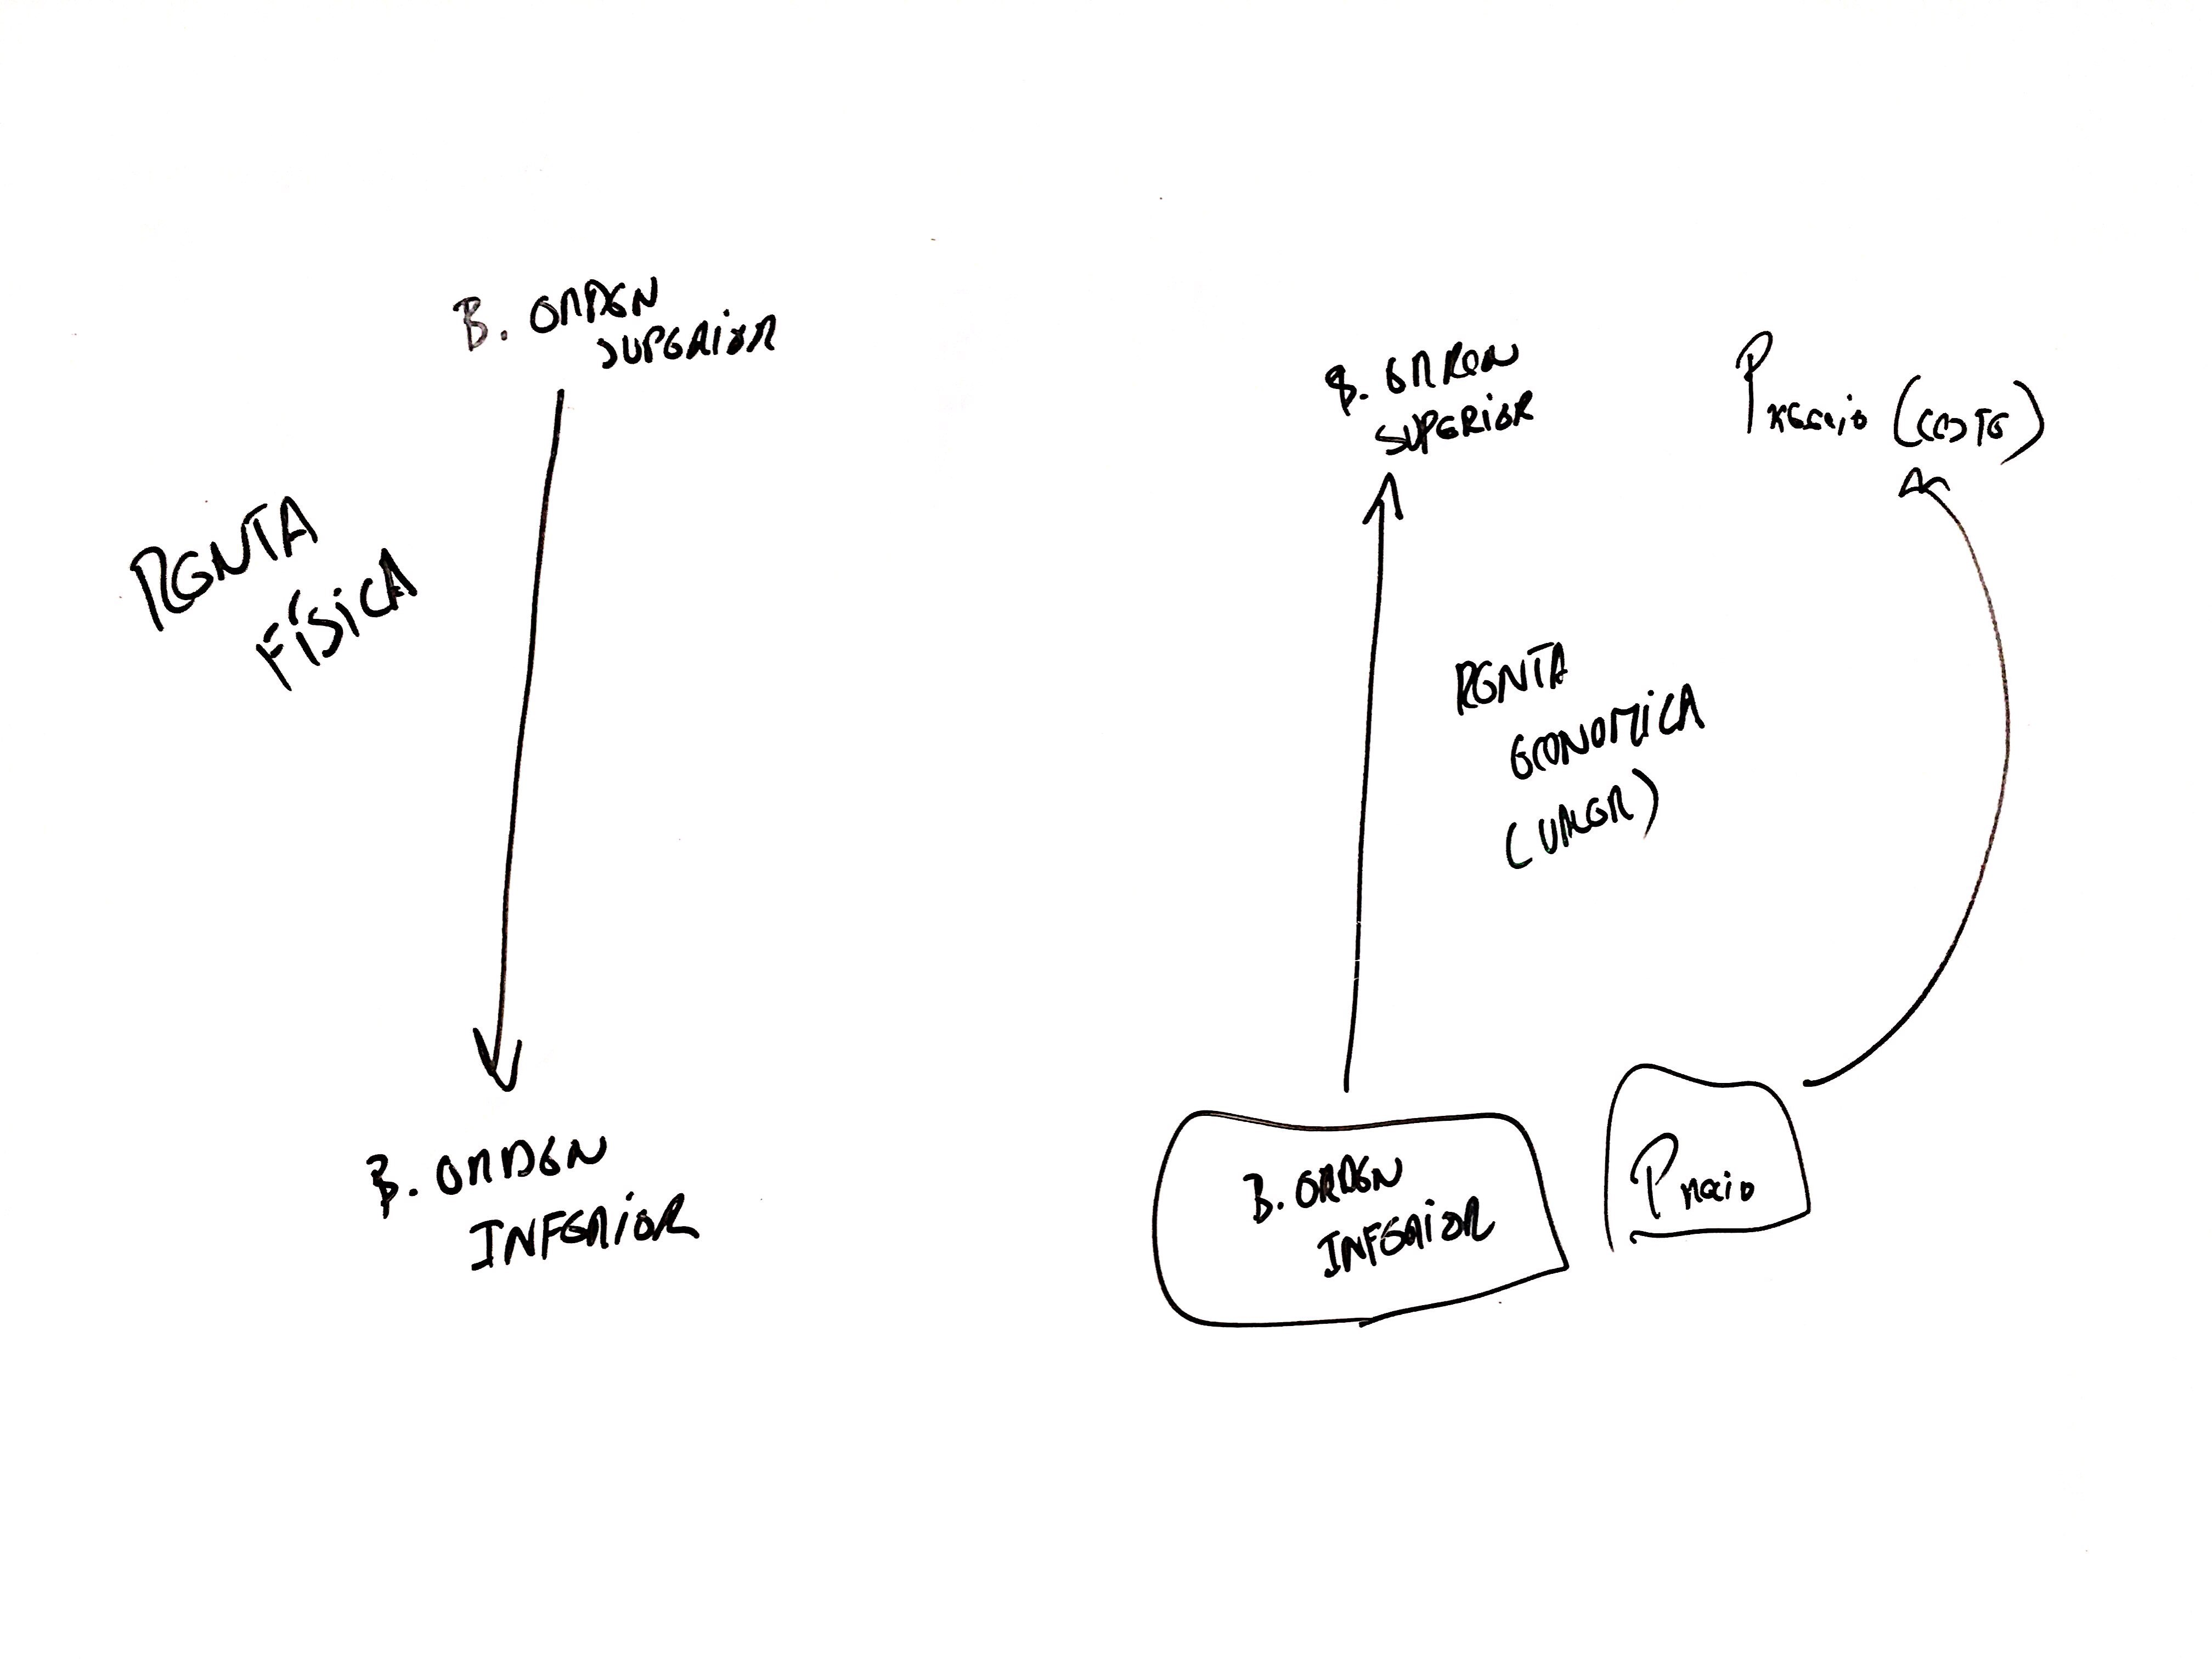
\includegraphics[width=10cm]{Classes/Images/2019-09-02-01.jpg}
    \caption{Renta física y renta económica}
    \label{}
\end{figure} 


\chapter{2019-09-04}
\section{Resolución de corto}
\begin{itemize}
    \item Ahorrar y después invertir en bienes de capital.
    \item Tienen más bienes de orden superior, ya tienen capital.
    \item El precio determina el costo.
\end{itemize}

\section{Noticia - La economía de españa está en peligro de una recesión}
\begin{itemize}
    \item Las cuentas nacionales: los países que invireten internacionalmente, \emph{\textbf{Definición de ``ingreso o egreso bruto":} es lo que ingreso o egresa.} \emph{\textbf{Definición de ``ingreso y egreso neto":} es la diferencia entre el ingreso y egreso bruto.}
    \item La prorroga de presupuesto no se actualiaza almenos que el gobierno se ponga de acuerdo. 
    \item PIM (purchasing manager index): indicador económico que se hace una encuesta a los compradores de empresas para ver si están comprando más que el mes pasado.
    \item Noticia, las condiciones para invertir se hace difícil.
\end{itemize}



\section{Discusión de clase}
\textbf{Dato*:} Se termina el tema de bienes.
\emph{\textbf{(Paréntesis:}Las empresas quiebran por que estiman precios mal. \textbf{\emph{(Ejemplo: El mercado de hule en GT, \textbf{Nos preguntamos:} ¿El proceso productivo del hule, cuánto dura?)}} Dura 5 años entonces el empresario debe especular 5 años y los acreedores que prestan a este especulador pueden estar sujetos a lo que pase en 5 años cuando esté el café\textbf{)}}

\begin{itemize}
    \item Repaso de bienes: los bienes de orden superior y de orden inferior la diferencia que tienen es mas que todo \textbf{tiempo}.
\end{itemize}

\begin{itemize}
    \item El interés es un precio, es por el tiempo, por el coste de oportunidad, etcétera.
    \[
      i_{M}= \underbrace{i_{\text{original}}}_{\text{precio del tiempo}} + \text{Prima riesgo} + \text{Prima de inflación}
    \]
    
    \item \emph{i} es el interés.
    \item \textbf{Prima de riesgo:} es como el límite interno, es una estimación de qué tan capaz de pagar devuelta el depósito y qué tanta buena fe tienes (historial de TDC). \emph{\textbf{(Paréntesis ``los bancos con nombres especializados'':}el banco industrial significa que le tiende a dar a las industrias préstamos\textbf{)}}
    \item \textbf{Prima de inflación:} La prima de inflación el porcentaged e inflación.
    \item \textbf{Prima de interés:} 
   \begin{figure}[htbp]
       \centering
       %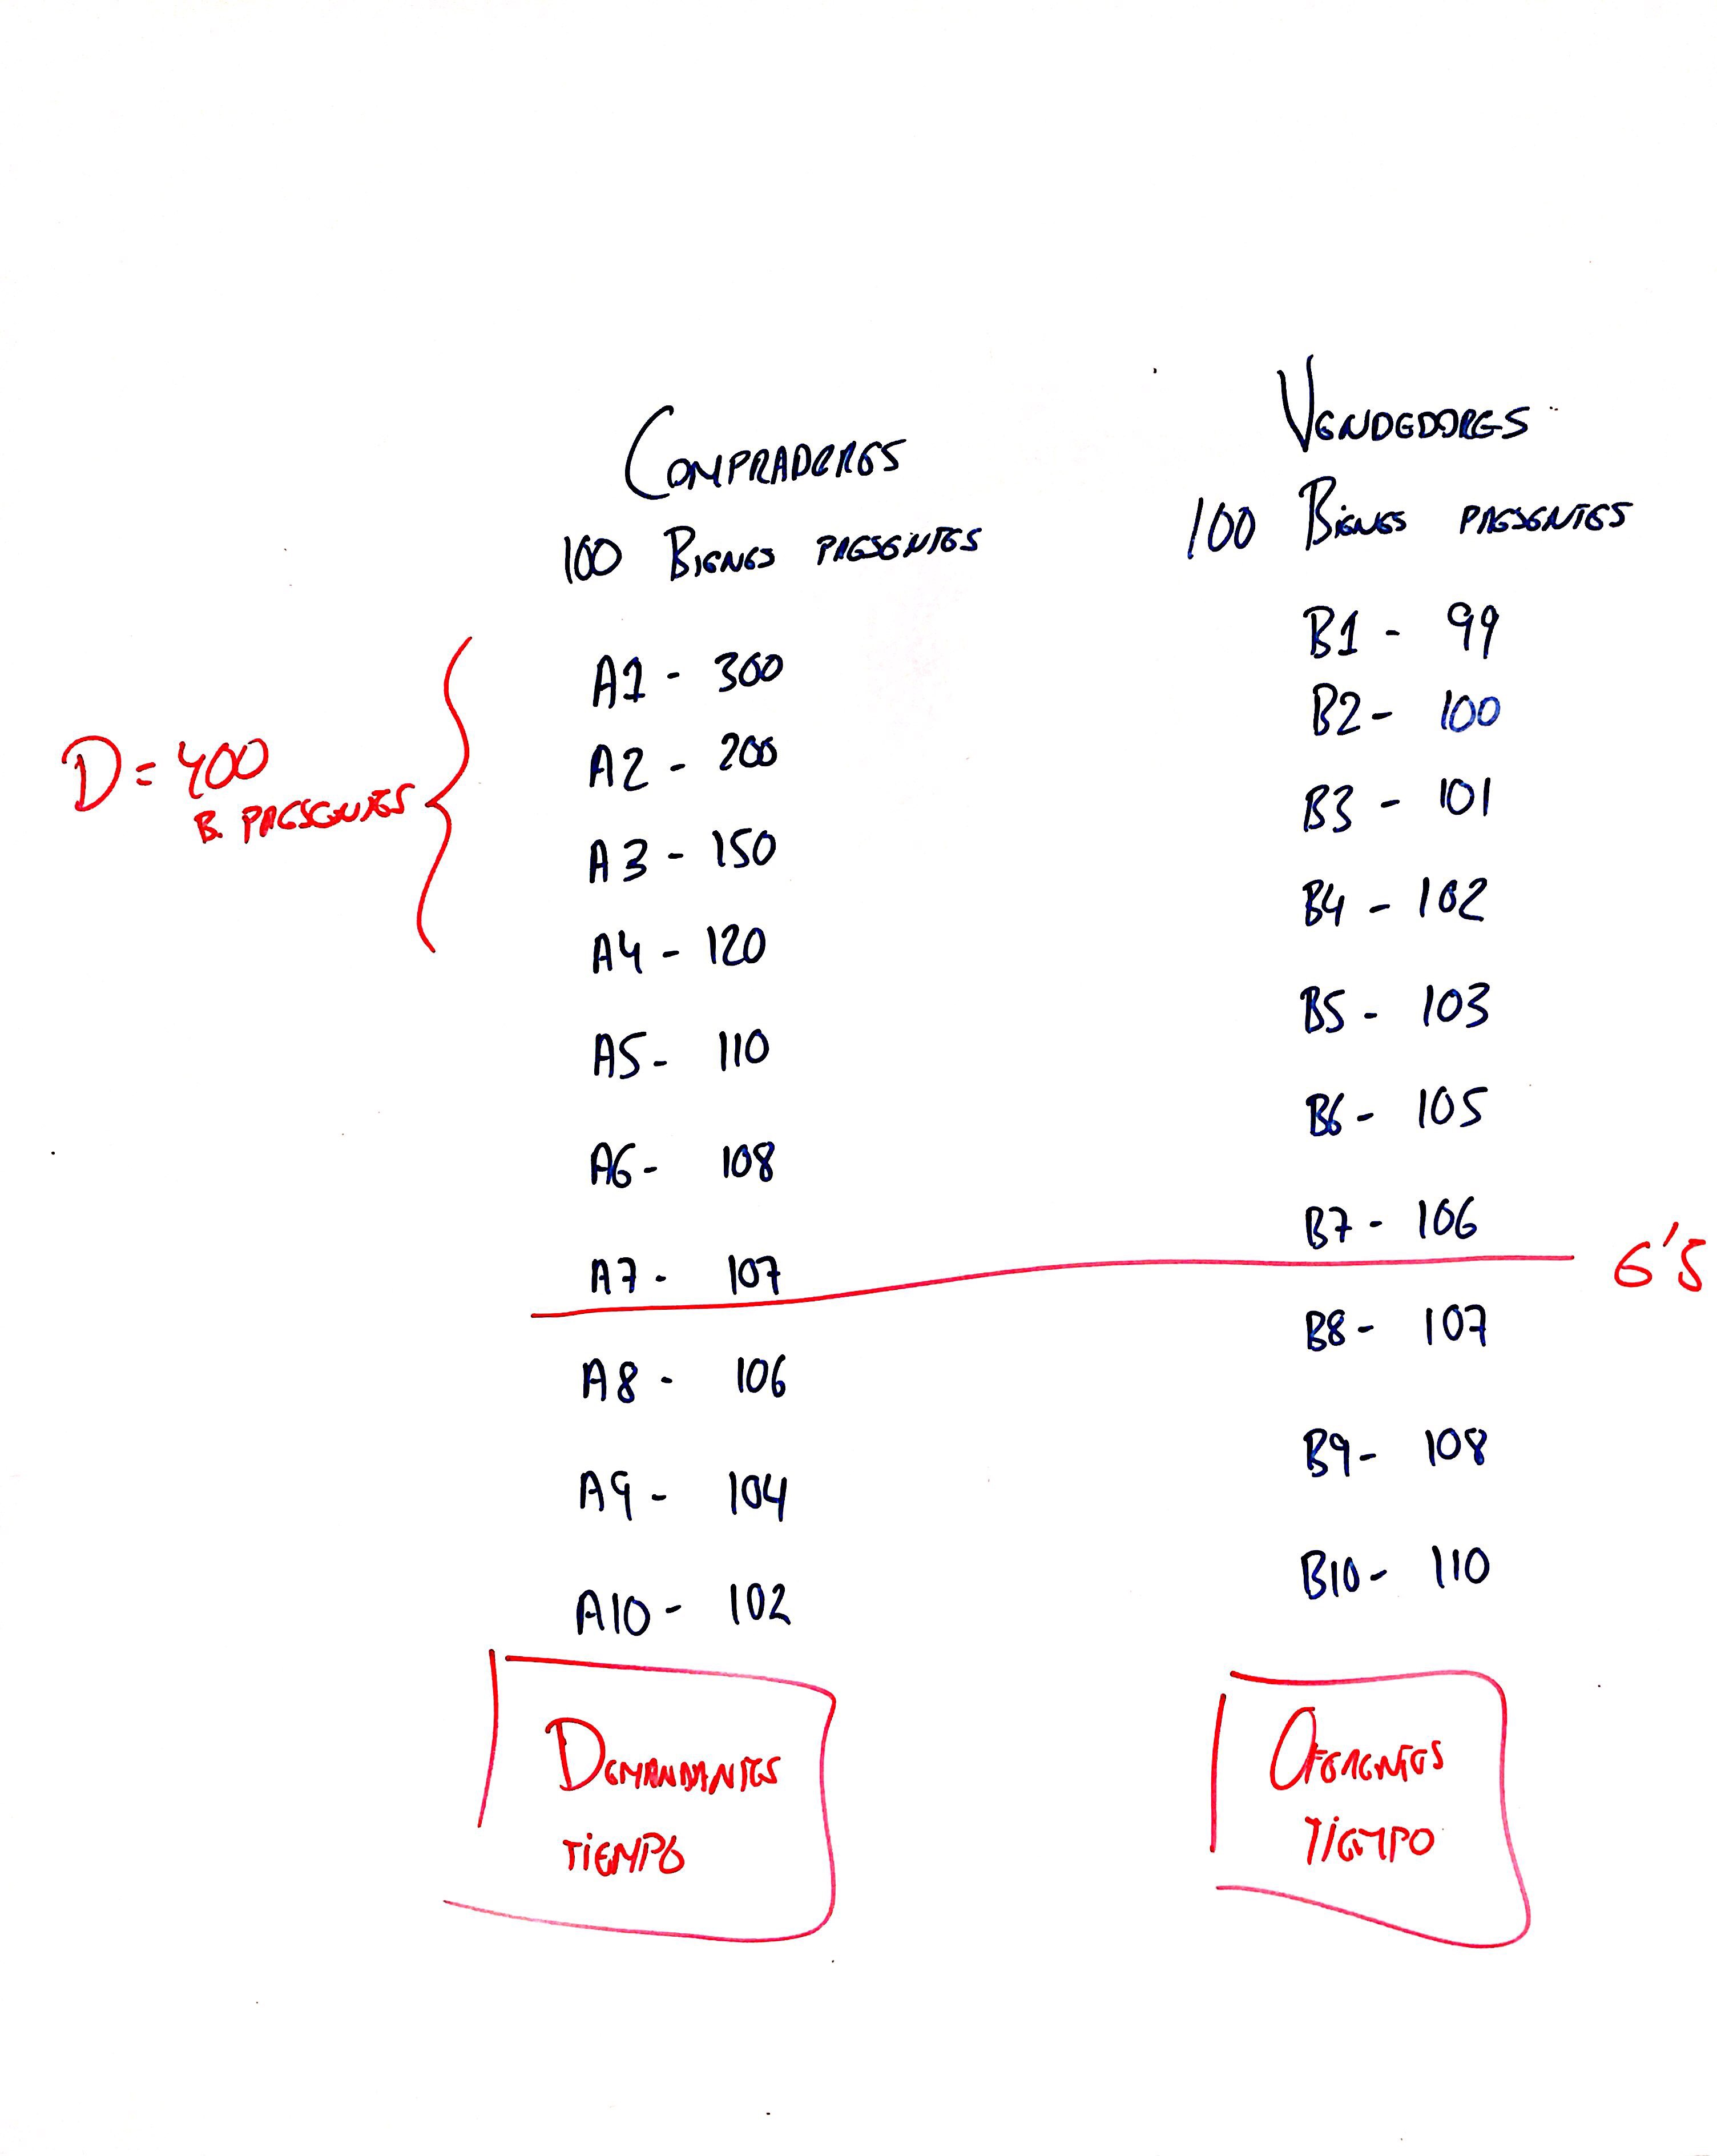
\includegraphics[width=6cm]{2019-09-04-01.jpg}
       \caption{}
       \label{}
   \end{figure} 
    
    \item La inflación beneficia al deudor, el pricipal es el estado.
    \item Veamos los oferentes del tiempo y los demandantes del tiempo.
    \begin{center}
    \begin{tabular}{ | p{5cm} | p{5cm} | }
     \hline
     Oferentes del tiempo (acreedores) & \\
     Demandantes del tiempo (deudores) & Empresarios (inversionistas) \\ 
     \hline
    \end{tabular}
    \end{center}
\end{itemize}



\subsection{Esquema de oferta y demanda de bienes presentes}
Las personas que valoran los bienes en el presentes especulando que en el futuro el bien prestado se va a aumenta respecto al interés.
\newline 
\textbf{\emph{(Ejemplo: el niño que espera 15 minutos por un nuevo dulce es un interes de 100\%)}} \emph{\textbf{(Paréntesis ``biología'':} la especie y su éxito recae en su capacidad de imaginarse en el futuro.\textbf{)}}
\begin{center}
\begin{tabular}{ | p{5cm} | p{5cm} | }
 \hline
  Compradores & Vendedores      \\
  100 Bienes presentes & 100 Bienes presentes \\ 
 \hline
    A1-300 & B1-99 \\ 
    A2-200 & B2-100 \\ 
    A3-150 & B3-101 \\ 
    A4-120 & B4-102 \\ 
    A5-110 & B5-103 \\ 
    A6-108 & B6-105 \\ 
    A7-107 & B7-106 \\ 
    A8-106 & B8-107 \\ 
    A9-104 & B9-108 \\ 
    A10-102 & B10-110 \\ 
\hline
    Demandante de tiempo & Oferentes de tiempo \\ 
\hline
\end{tabular}
\end{center}

\begin{itemize}
    \item Una onza de oro ha valido por lo general es suficiente para un mes.
    \item Mercado intertemporal.
    \item Para el interes se paga con bienes presentes respecto a la valoración subjetiva que cada uno espere recibir en el futuro.
    \item El que pone en contacto a los compradores y vendedores es el sector bancario.
\end{itemize}

\begin{figure}[htbp]
    \centering
    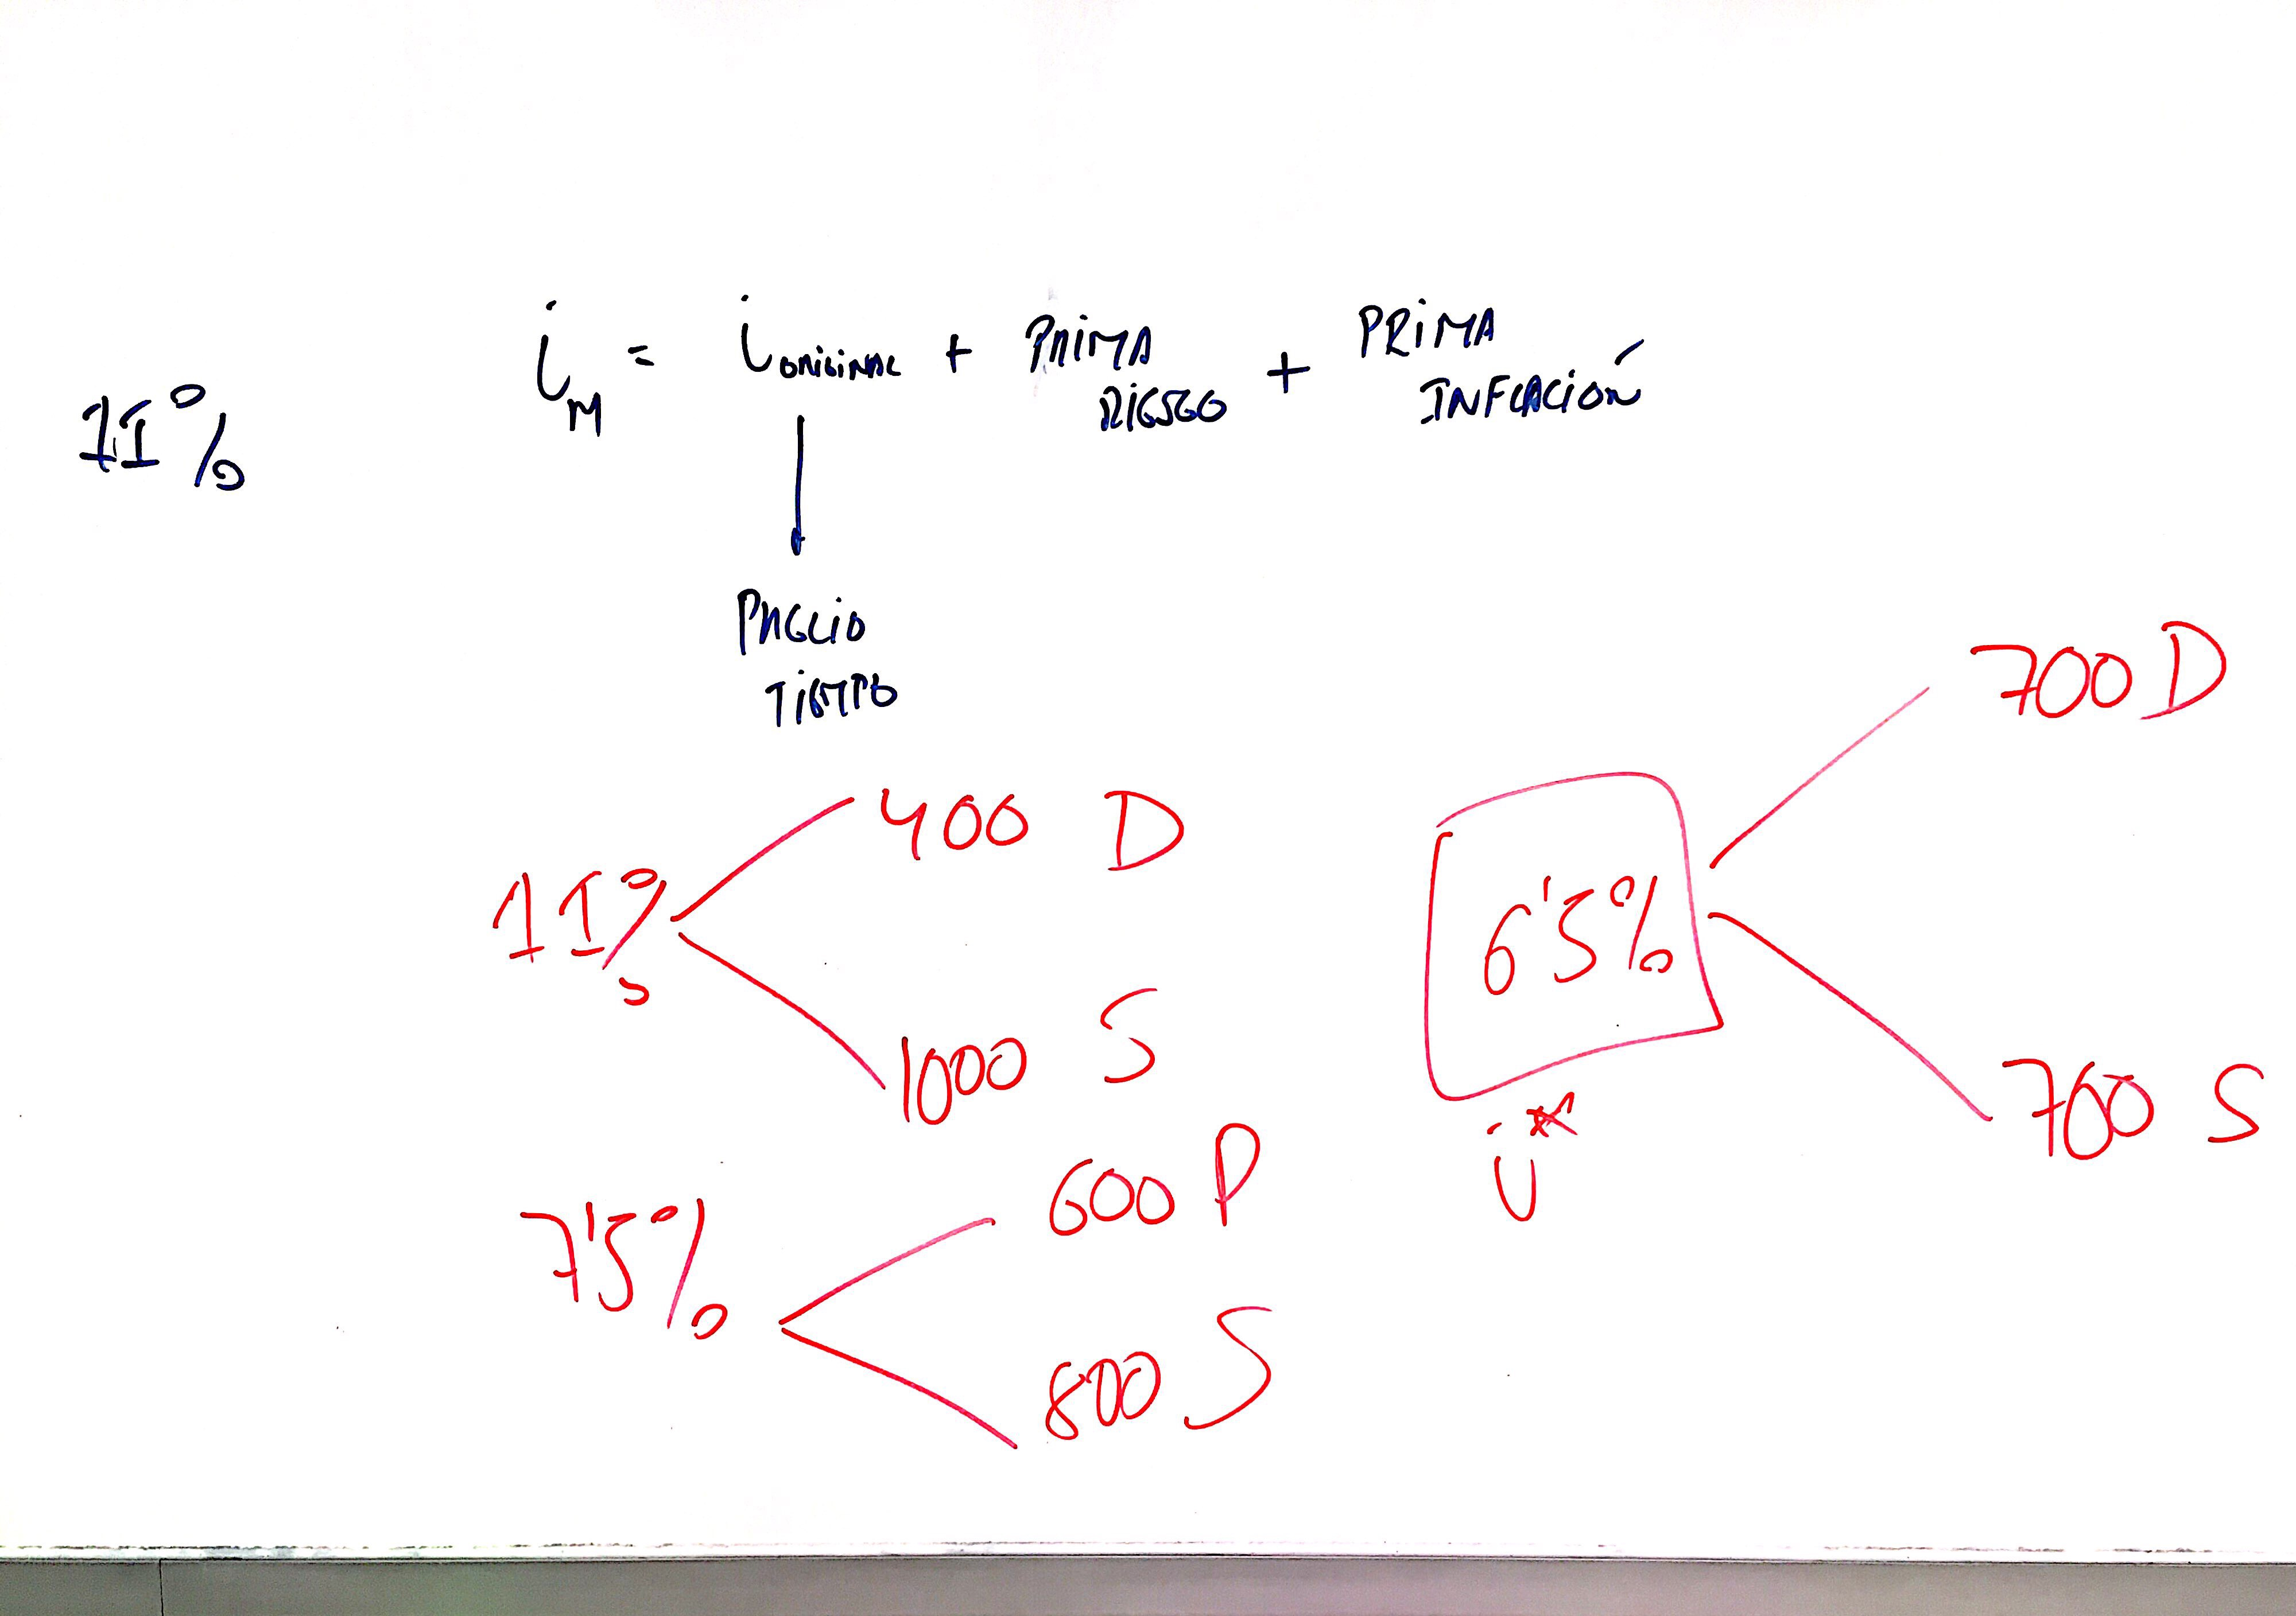
\includegraphics[width=6cm]{Classes/Images/2019-09-04-02.JPG}
    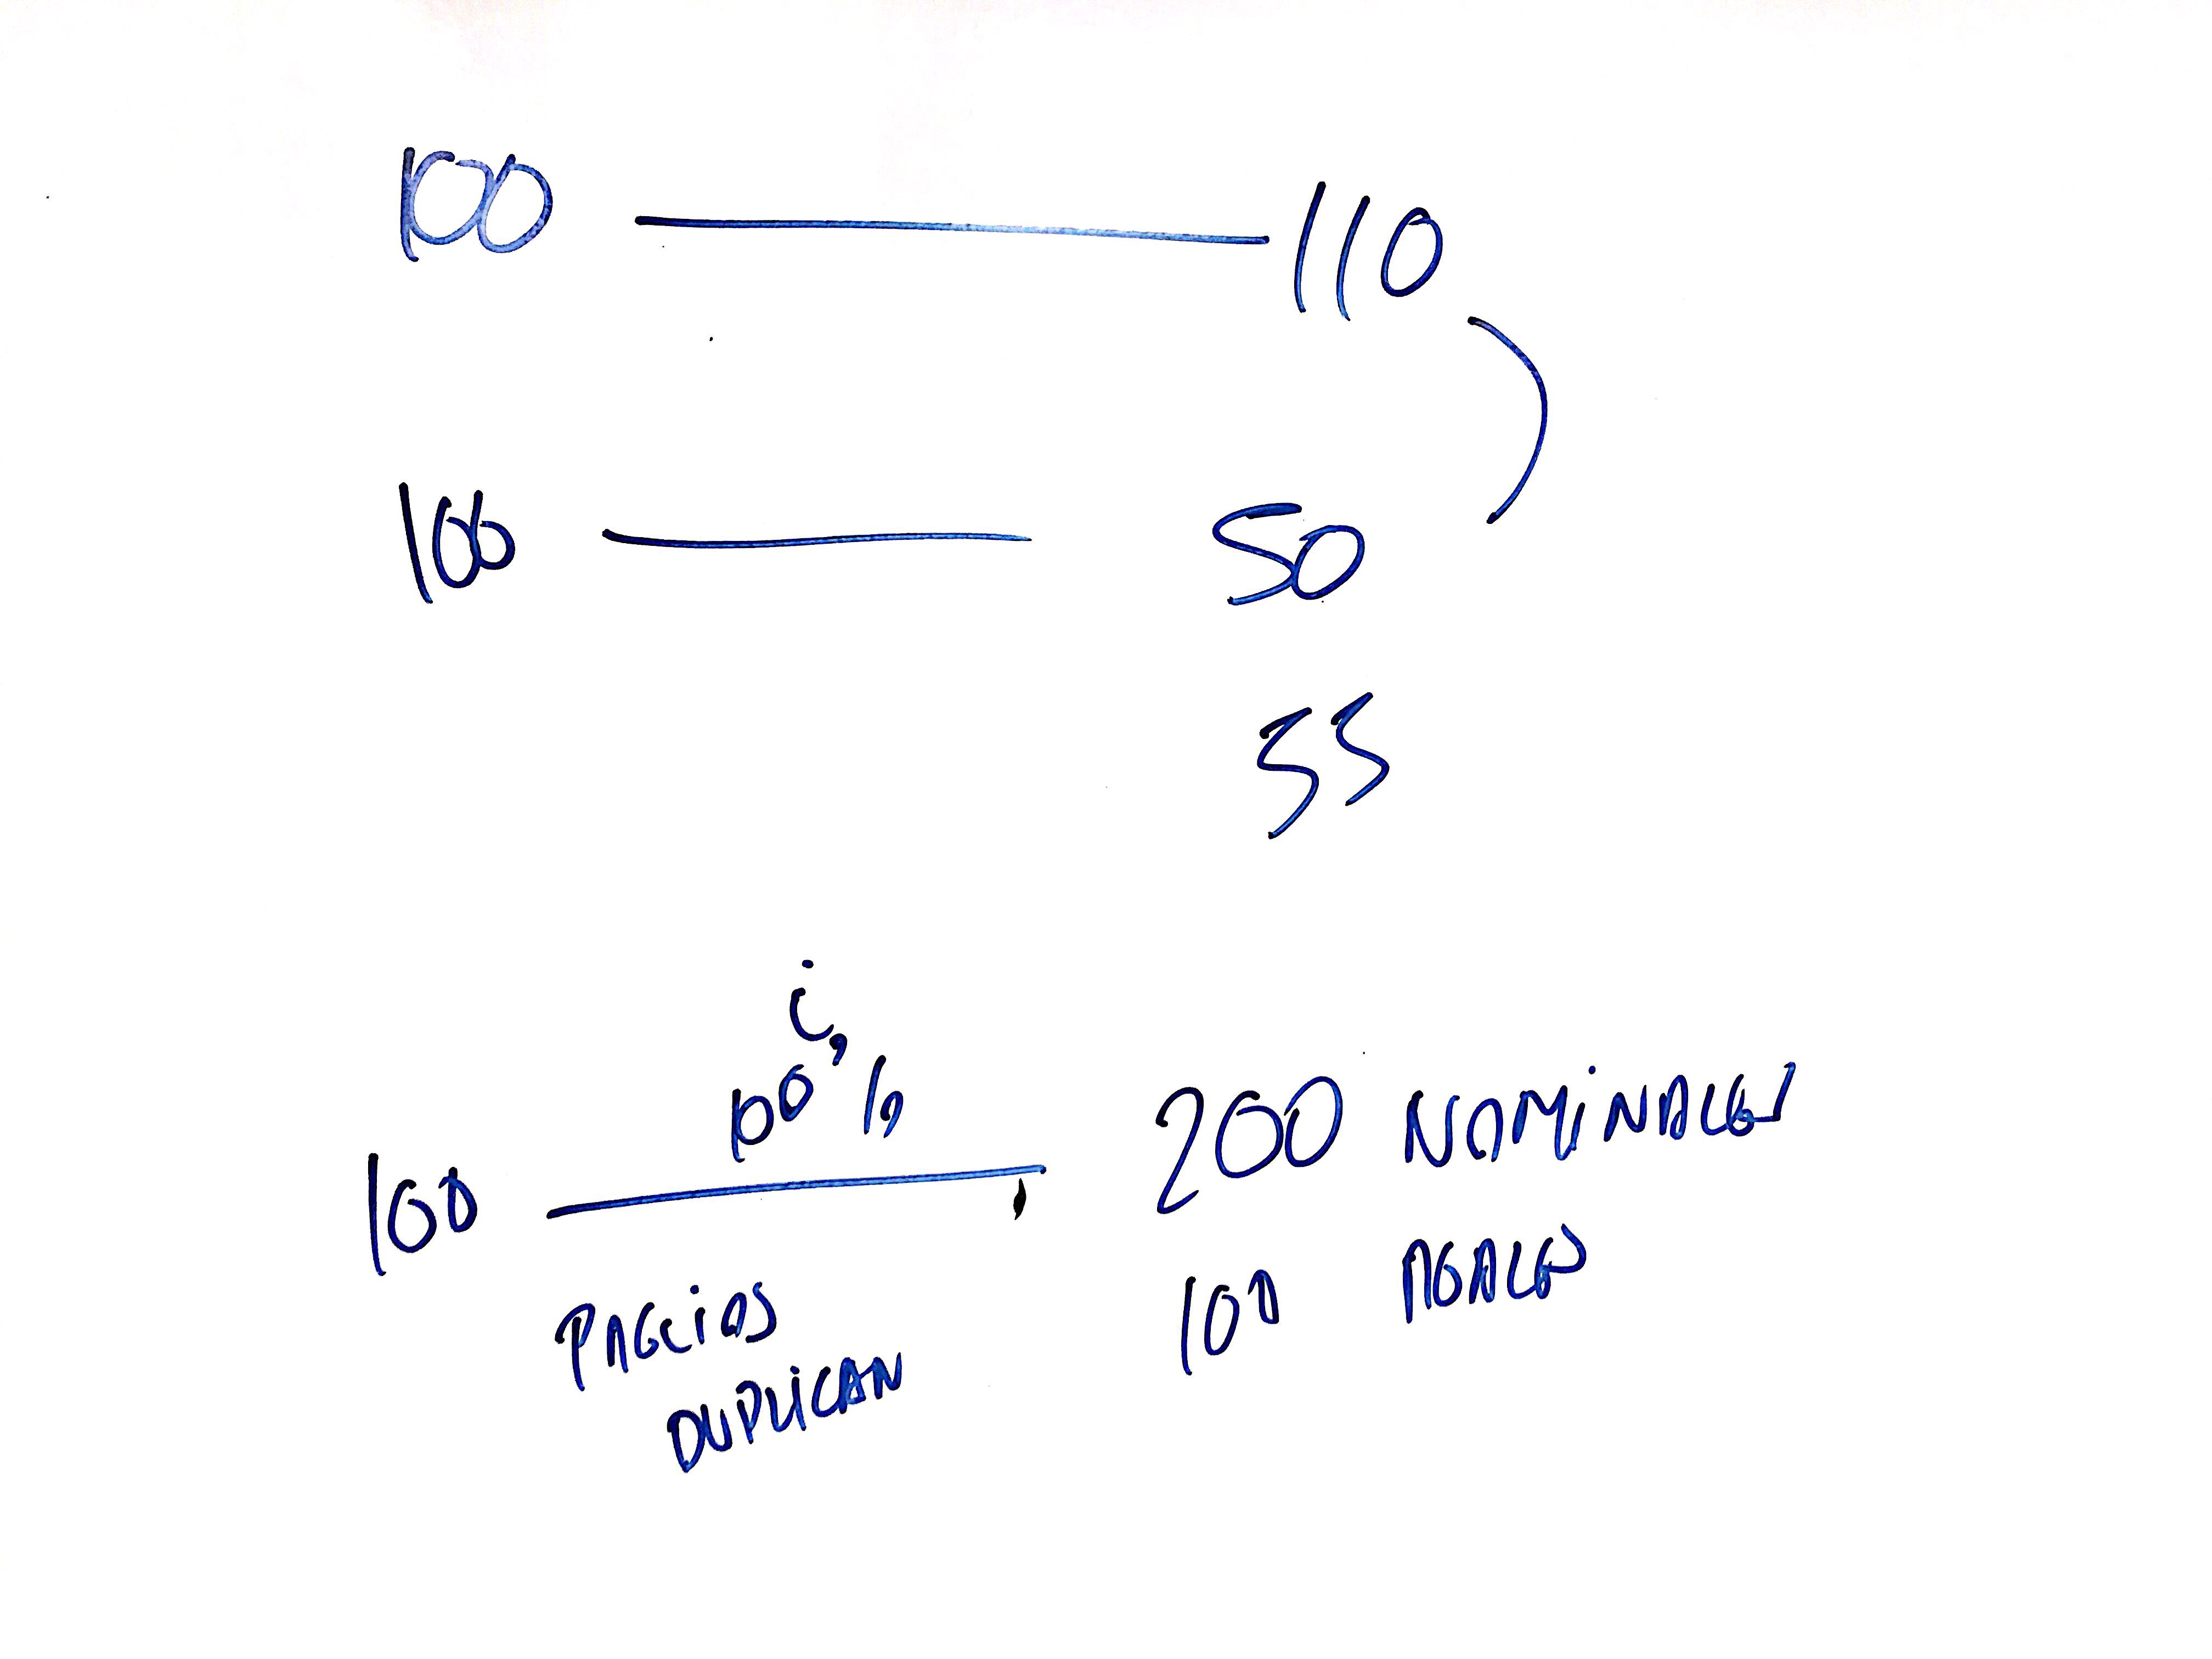
\includegraphics[width=6cm]{Classes/Images/2019-09-04-03.JPG}
    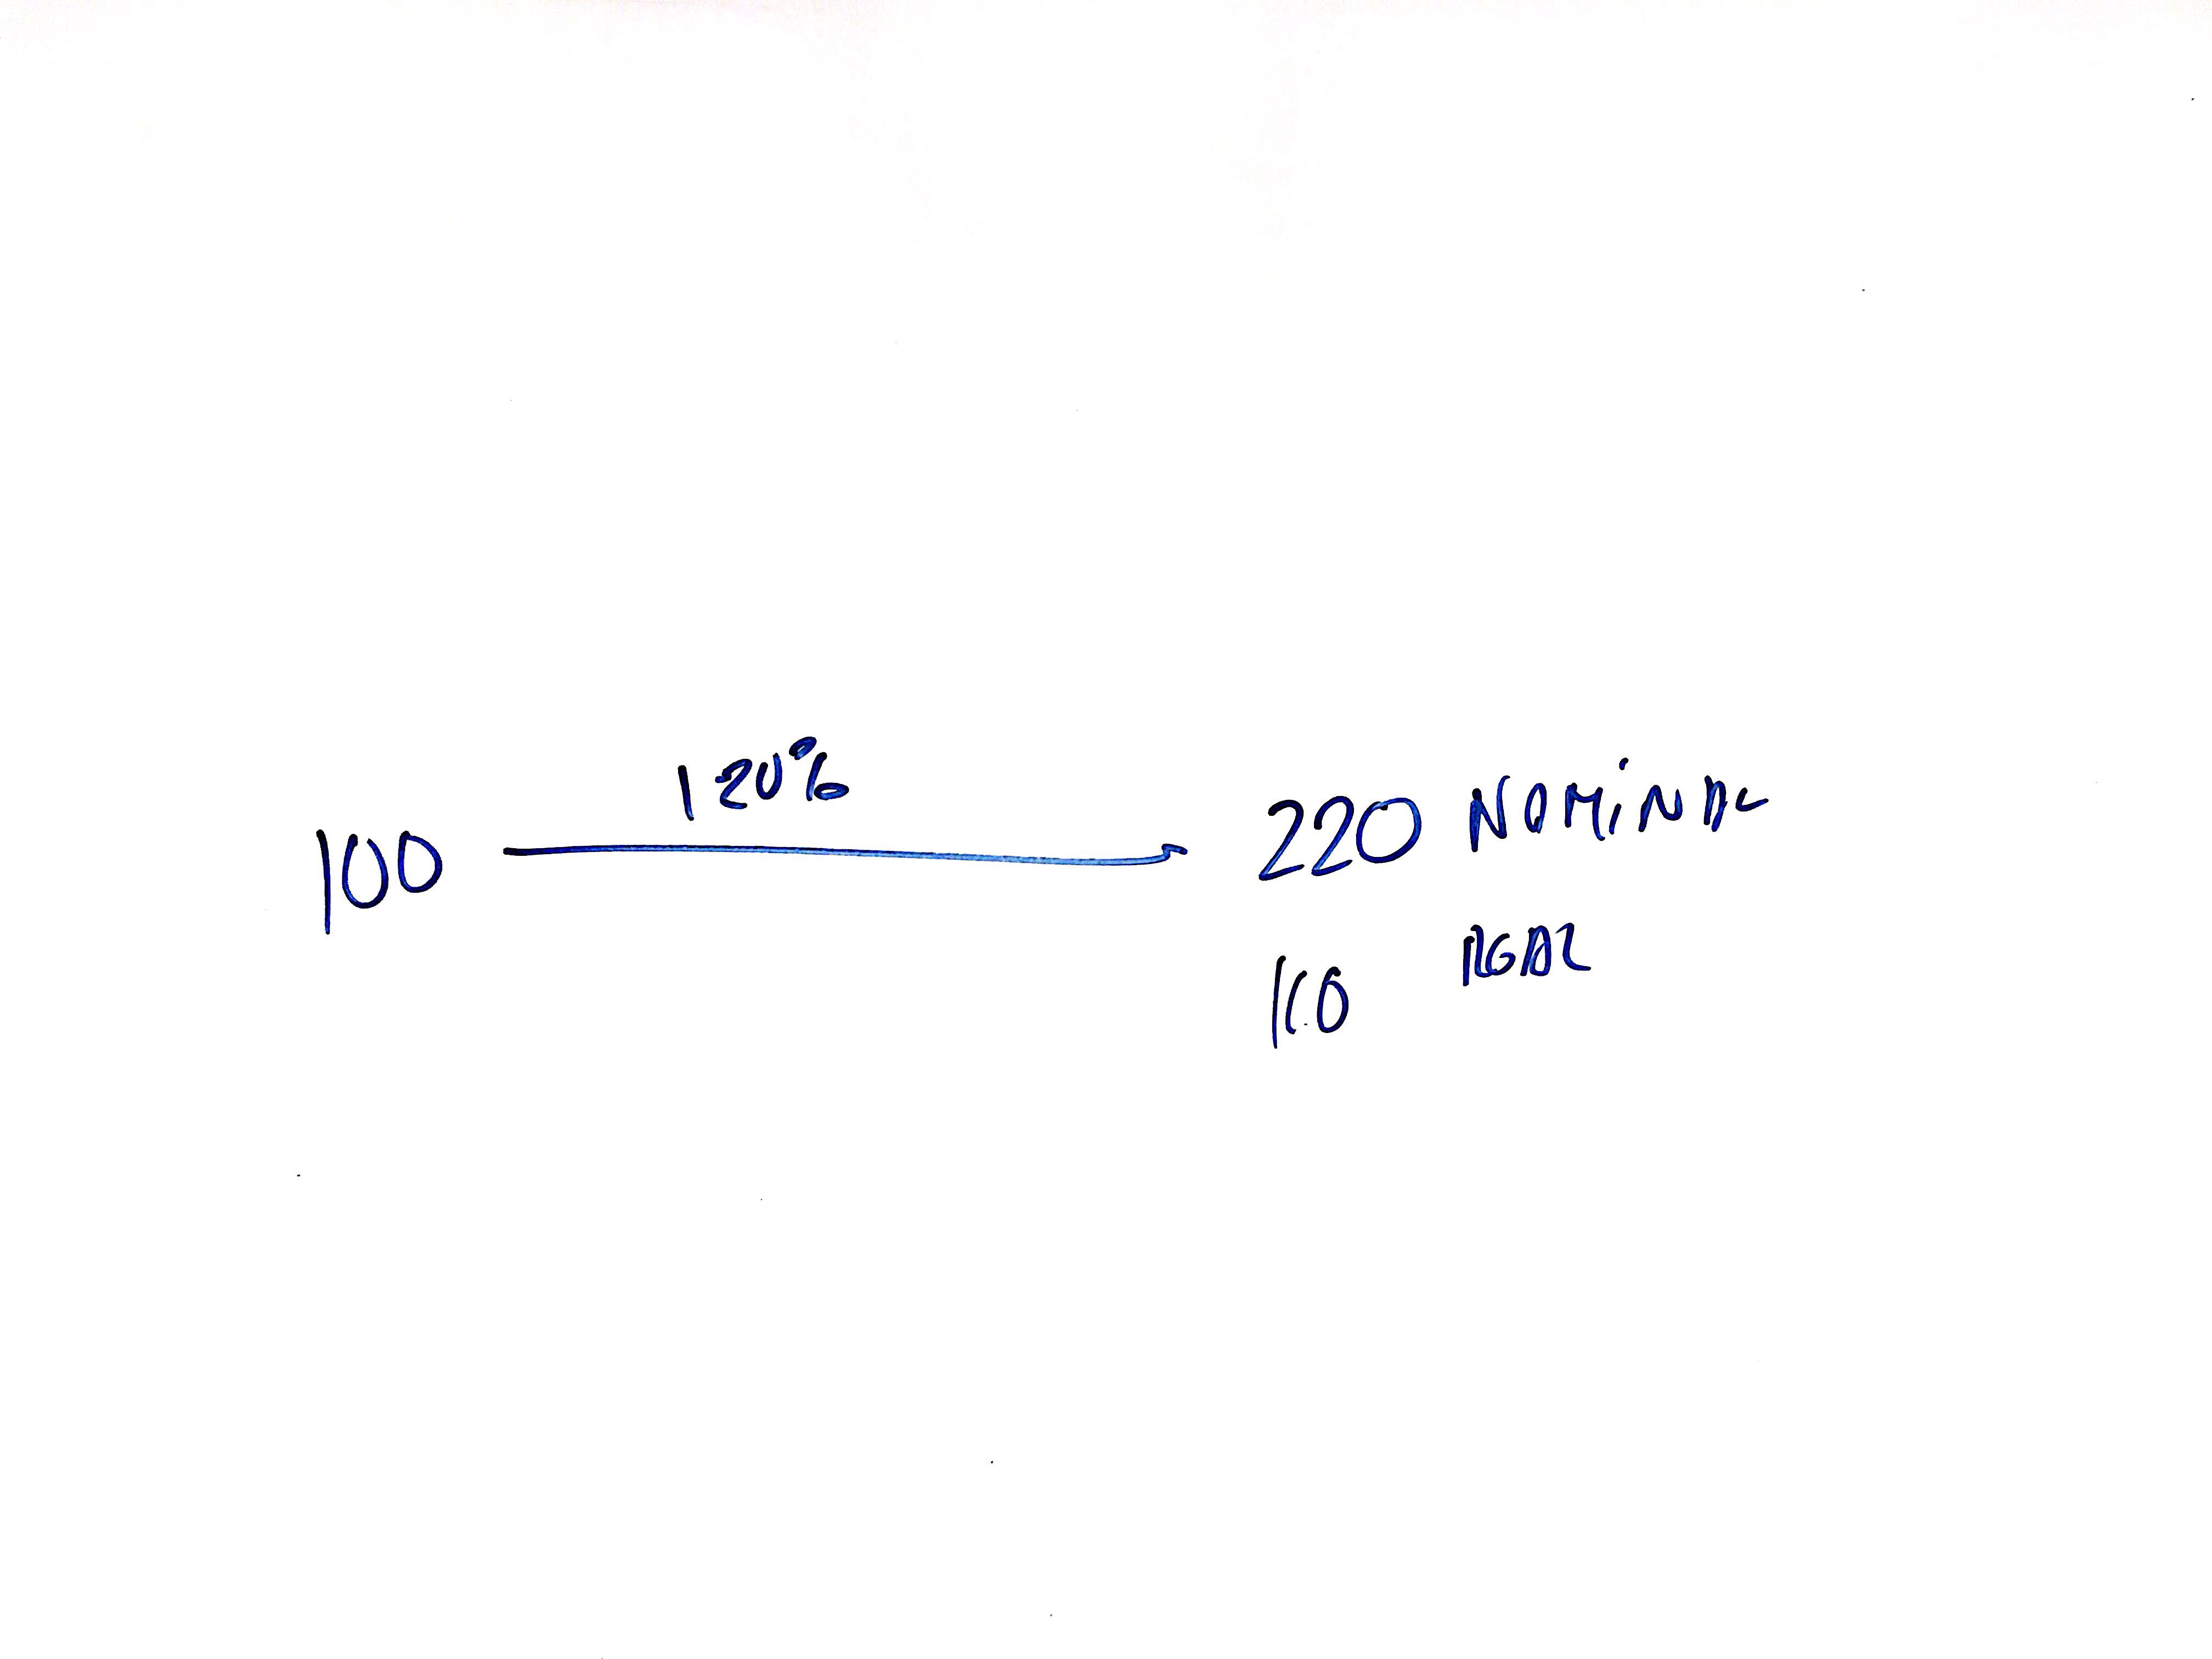
\includegraphics[width=6cm]{Classes/Images/2019-09-04-04.JPG}
    \caption{}
    \label{}
\end{figure} 

\begin{figure}[htbp]
    \centering
    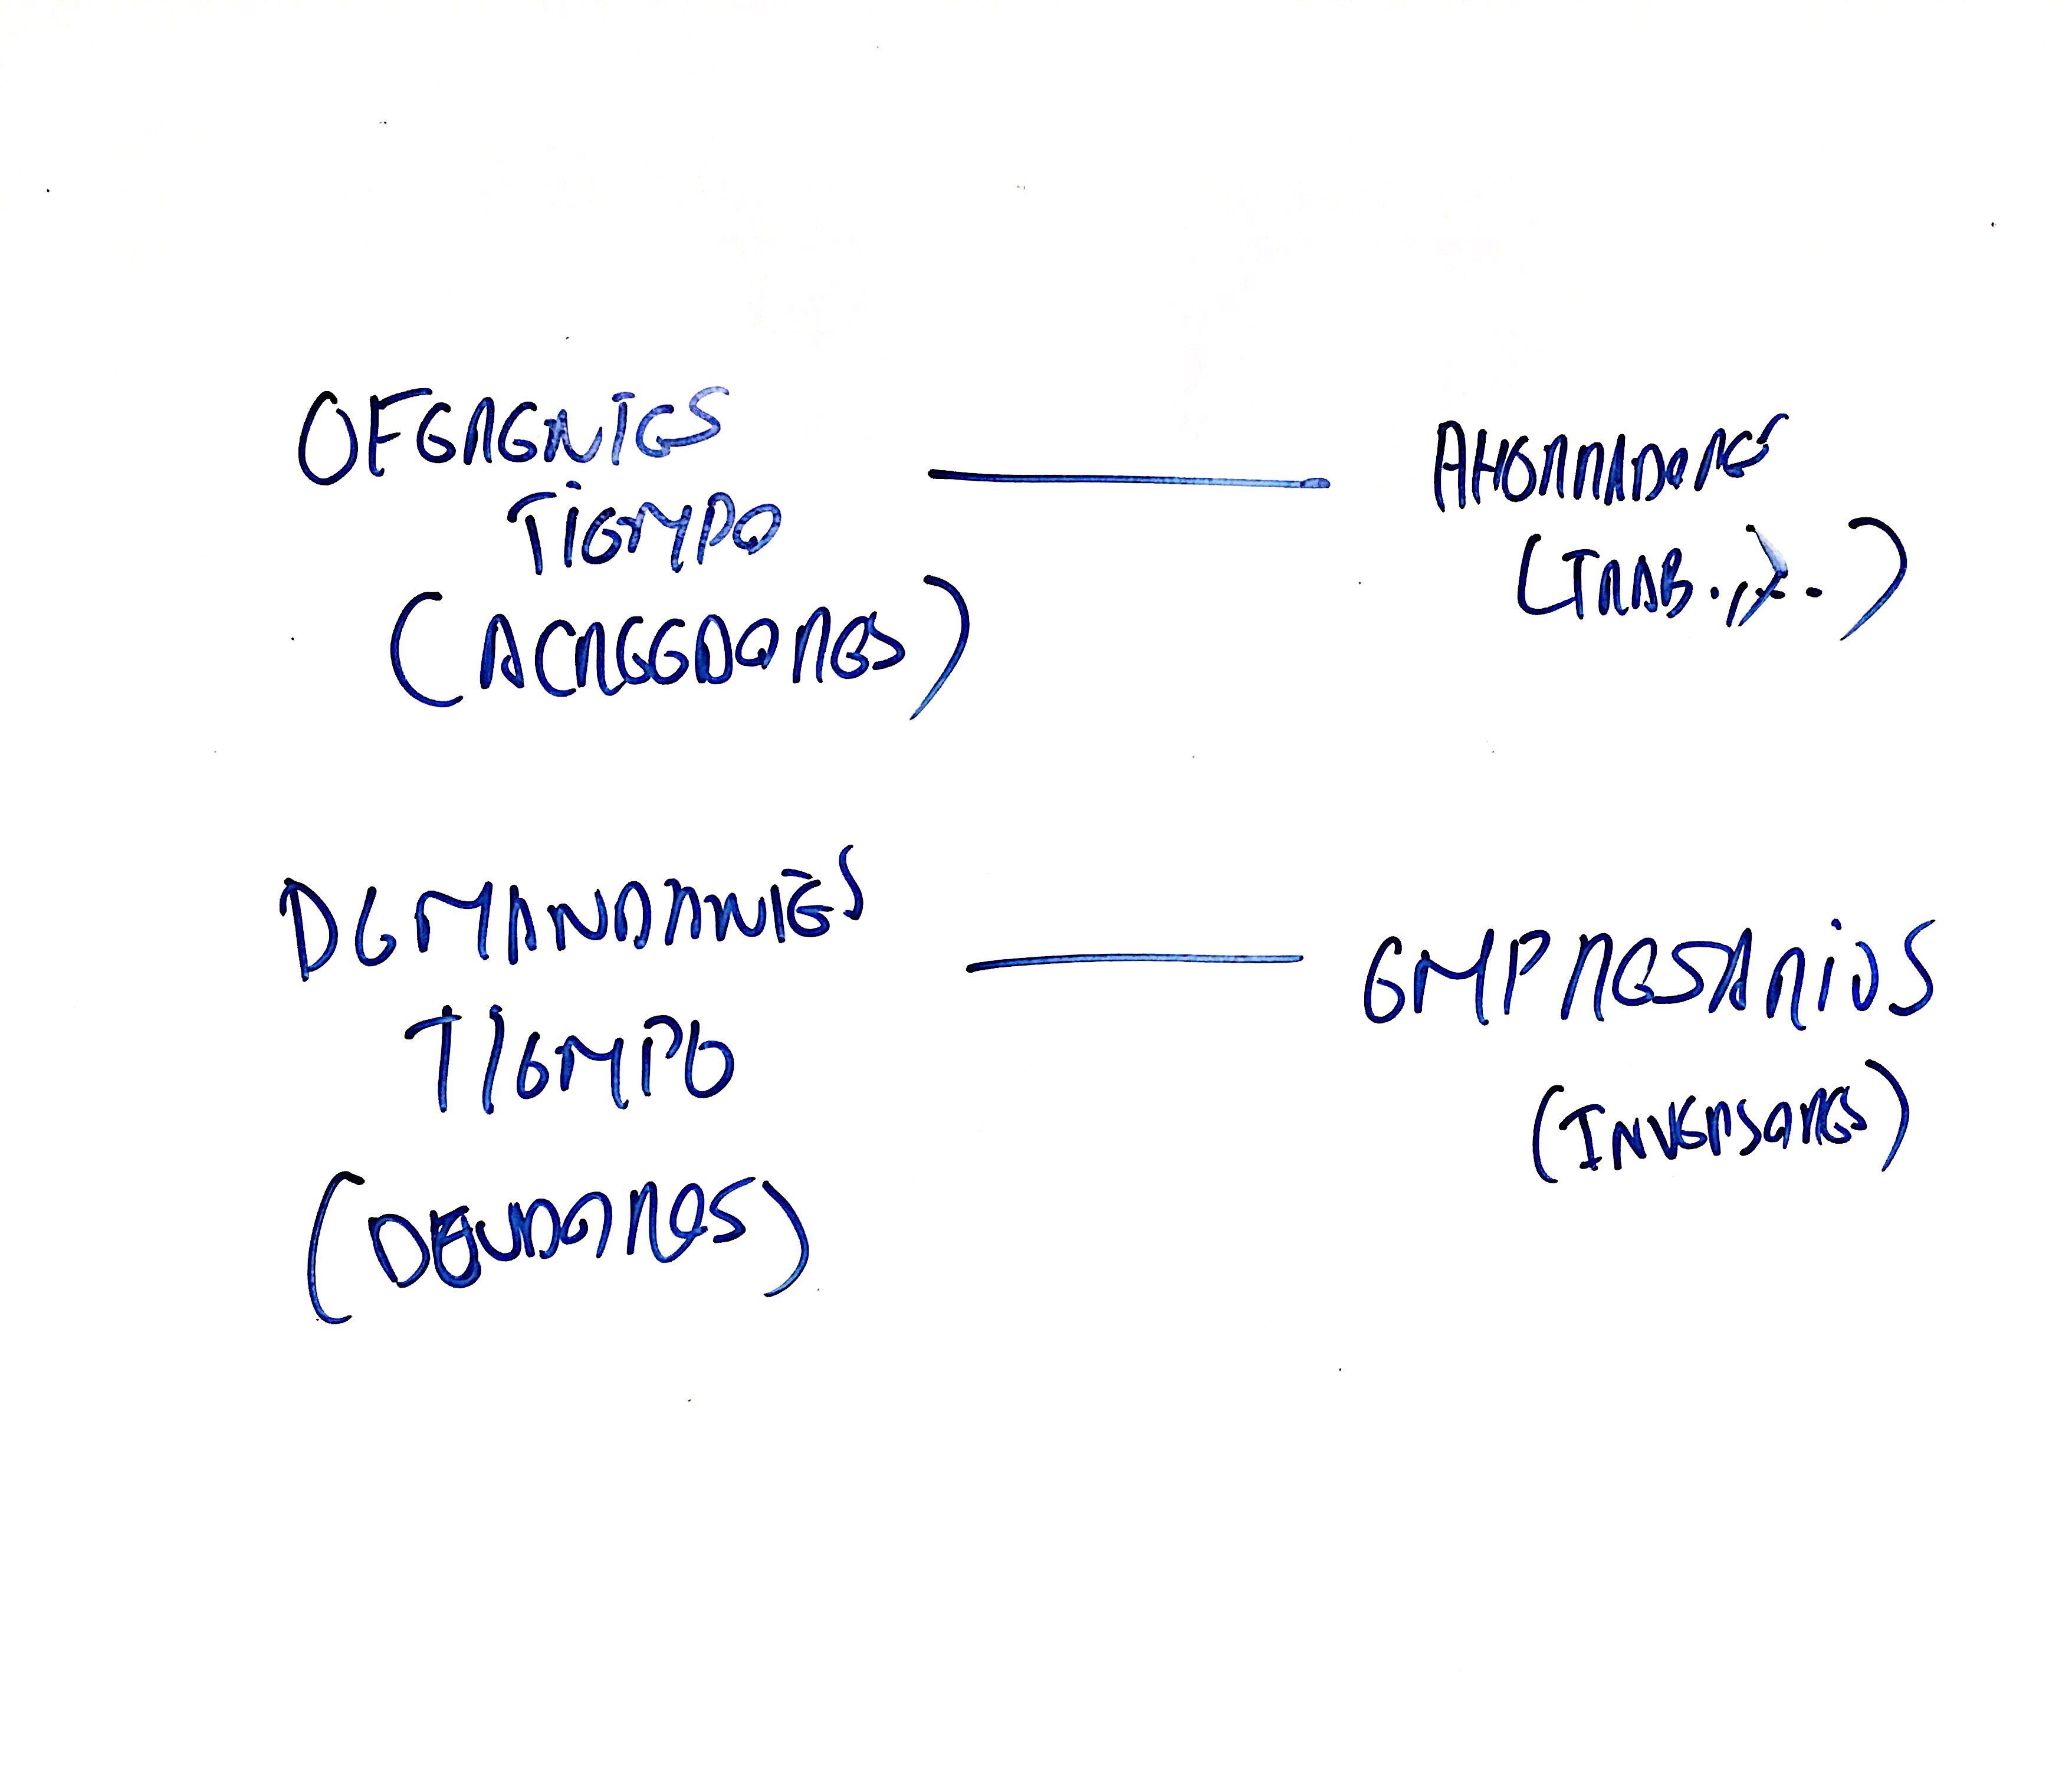
\includegraphics[width=6cm]{Classes/Images/2019-09-04-05.JPG}
    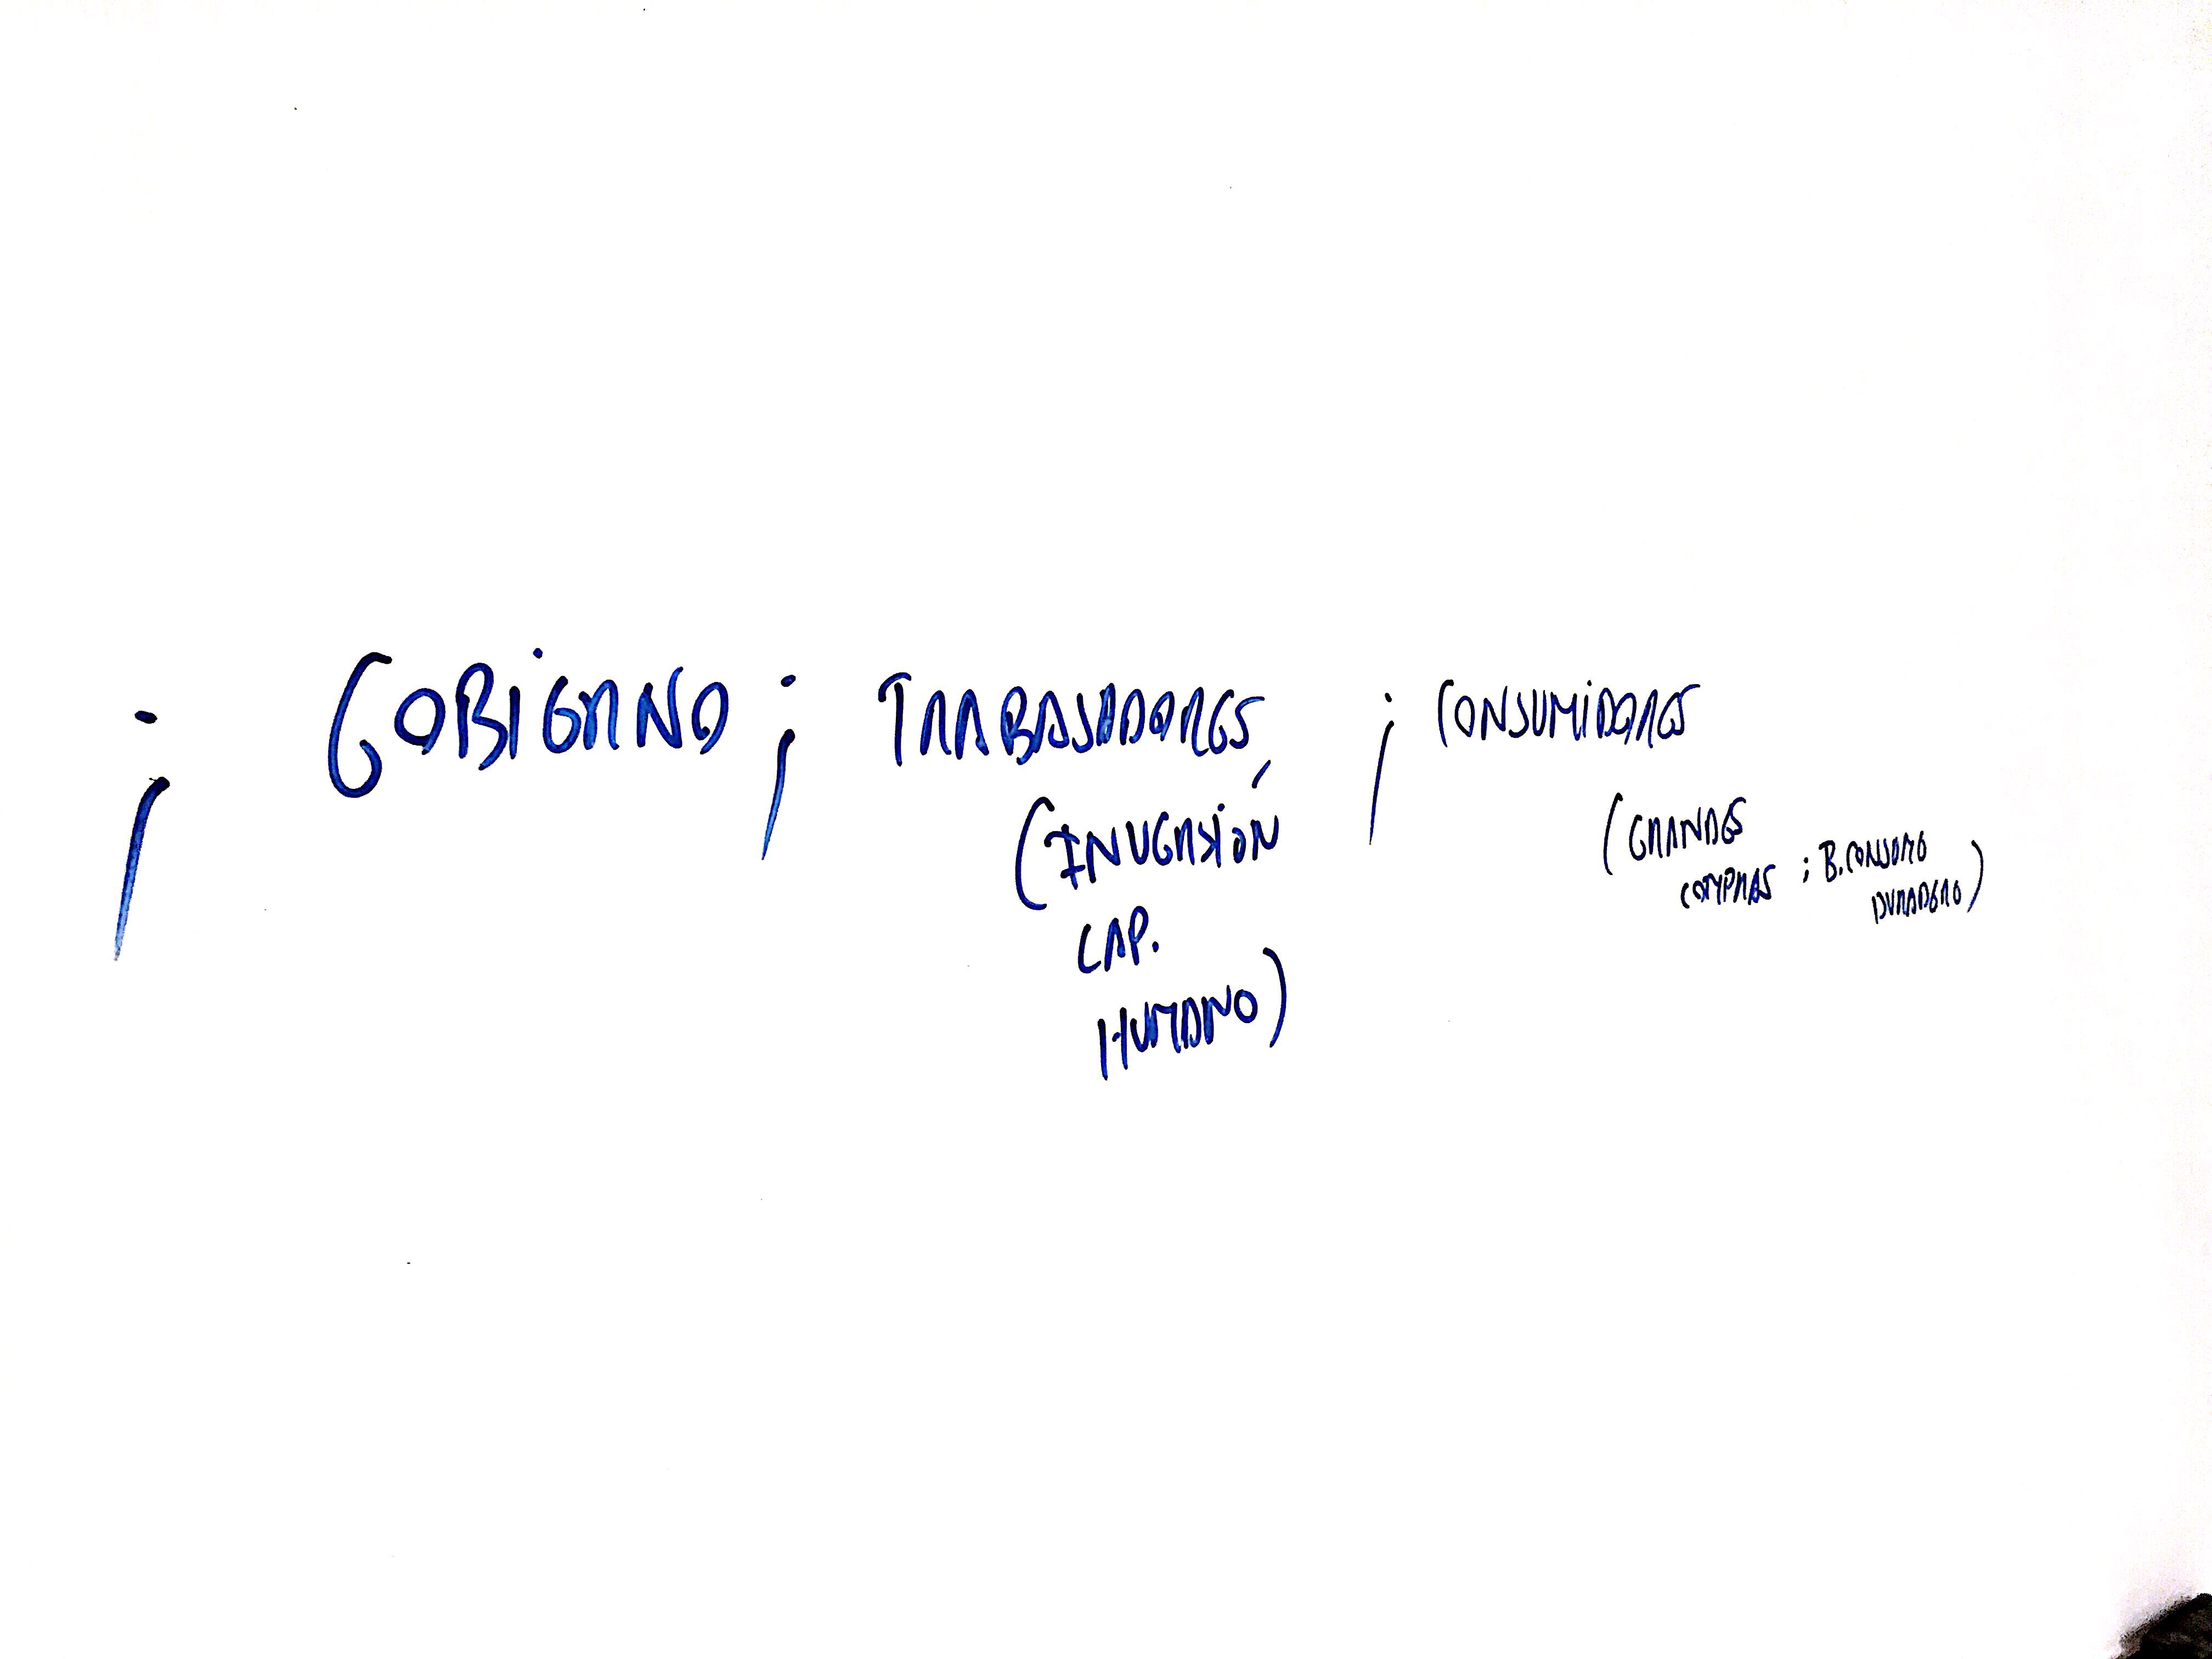
\includegraphics[width=6cm]{Classes/Images/2019-09-04-06.JPG}
    \caption{}
    \label{}
\end{figure} 




\chapter{2019-09-09}
\section{Noticia de aguas y proyecto}
\begin{itemize}
    \item Proyecto Bill Gates 
    \item Proyecto de purificación de agua 
\end{itemize}


\section{Discusión de clase}
\begin{itemize}
    \item \emph{\textbf{(Paréntesis ``La idea de una máquina que produzca energía infinita'':}Hasta ahora no existe.\textbf{)}}
\end{itemize}

\begin{tabular}{ | p{5cm} | p{5cm} | }
    \hline
     Compradores & Vendedores      \\
     100 Bienes presentes & 100 Bienes presentes \\ 
    \hline
       A1-300 & B1-99 \\ 
       A2-200 & B2-100 \\ 
       A3-150 & B3-101 \\ 
       A4-120 & B4-102 \\ 
       A5-110 & B5-103 \\ 
       A6-108 & B6-105 \\ 
       A7-107 & B7-106 \\ 
       A8-106 & B8-107 \\ 
       A9-104 & B9-108 \\ 
       A10-102 & B10-110 \\ 
   \hline
       Demandante de tiempo & Oferentes de tiempo \\ 
   \hline
\end{tabular}


\begin{itemize}
    \item En la tabla anteriormente presentadas:
    \begin{itemize}
        \item \textbf{\emph{(Ejemplo:}}\emph{ Ejemplo alternativo: Estas en un bar, estas tomando algo y un amigo está hablando con una amiga muy guapa, cuando estoy \textbf{picado} tengo preferencia temporal \textbf{alta}, mi amigo tiene que pagar su cerveza y la de la amiga, el incentivo personal es 2 - 1 \& 4 - 1, mi amigo me pide pagar dos en el futuro por el dinero para pagar una cerveza hoy; el amigo se endeuda en cervezas, el tipo de 4 - 1 es muchísimo más impaciente porque pagará  tres cervezas más en el futuro por una hoy. Dependiendo de la circunstancia las personas van a demandan más o menos bienes presentes por bienes futuros.)}
        \item \textbf{Nos preguntamos:} ¿qué pasa cuando una economía tiene gente muy impaciente? El interés sube ya que más demanda por bienes presentes y mayor disposición de pago en bienes futuros. Los países pobres tienden a ser muy impacientes, ¿por qué? \textbf{no pueden ahorrar}. En el primer mundo es fácil ahorrar, en el tercer mundo implica pasar hambre.
        
        \item \textbf{Nos preguntamos:} ¿Una economía de mucho emprendimiento tiene un interés alto o bajo? El interés tiende a ser elevado ya que mayor gente demanda bienes presentes para invertir hoy y pagar después. En las recesiónes económicas el interés tiende a caer.

        
        \item Mientras más arriba estoy más ahorro
        \item El banco central tiende a tener mucho miedo a que suba el interés y mucho incentivo a querer bajarlo. El banco es solo un intermediario entre los oferentes o demandantes. ¿Por qué? por que estimula la economía para que personas lleven a cabo sus proyectos productivos, por consiquientes se hacen rentables, por consiguiente se provoca un boom económico, los proyectos de bajo valor agregado empiezan a surgir y entonces todo esto produce.
        \item En los interéses bajos se produce más demanda y menos oferta, al claramente estar en \textbf{desquilibrio}, el banco compensa este diferencial con la creación de dinero, por ende el que gana es el banco por la inflación producida retardada y el interés ``bajo'' se queda igual. 
        \item En cuanto se baja el interés se estimula la economía y después para compensar inflan la moneda.
        \item Estimula la economía a coste de la ilusión de interéses bajos, el retardo fluctúa entre 18-24 meses.
        \item \emph{Citación:``La inflación es un impuesto oculto (por esto, creyendo que el interés es más bajo invierten pero tras tomar en cuenta de la inflación es un engaño)"} 
    \end{itemize}
\end{itemize}


\chapter{2019-09-16}
\section{Presentaciones finales}
\subsection{MP}


\chapter{2019-09-18}
\section{Resolución del corto}
\begin{enumerate}
    \item Solo se toma en cuenta los bienes finales para no contabilizar dos veces el mismo bien.
    \item Se calcula la infomalidad con las diferentes fórmulas de calcular el PIB.
    \item Problemas del uso del PIB: no toma en cuenta el auto-consumo, auto-producción, actividades domésticas.
    \item Por qué el PIB es engañoso en las guerras:
    \begin{itemize}
        \item Aumenta la producción de bienes destinados a destruir riquezas.
        \item \emph{Citación:``En una guerra gana el que más capacidad tenga de producir"}
        \item El PIB aumenta pero no genera riqueza, usualmente se usa el PIB para medir riqueza.
    \end{itemize}
\end{enumerate}

\section{Noticia}
\textbf{Nos preguntamos:} ¿Los robots remplazarán a las personas trabajando?
\begin{enumerate}
\item \emph{\textbf{Definición de ``Producción":} Cantidad de output respecto a la cantidad de input}
\item Se ven ventajas al trabajar con robots, la automatización aumenta la producción.
\item Premisa a que el mercado va a hacer albitraje al estudiar cómo reparar, hacer, etcétera los robots de automatización, se va a especializar en diferentes capacidades.
\item \textbf{Nos preguntamos:} ¿La riqueza solo se concentrará en una pequeña parte de la población capacitada en automatización? A corto plazo sí, pero a largo plazo no.
\end{enumerate}

\section{Discusión de clase}
\begin{enumerate}
    \item Relacionando a el tema de la noticia: \textbf{Nos preguntamos:} ¿dónde se analfebetizó de primero? Francia e Inglaterra, por que su mano de obra era especializada en educación privada. Cuando llegó la necesidad de más mano de obra especializada lo primero que se invirtió en fue en educación.
    \item \emph{\textbf{(Paréntesis ``Censo'':}en GT se pretendía que tenía 17M pero son 15M\textbf{)}}
    \item Ludismo, analfabetismo.
    \item La automatización es una problemática similar a la que pasó con la revolución industrial por ende la automatización no pronostica que la automatización vaya a devastar todo.
    \item La revolución industrial mejoró la calidad de vida, \emph{\textbf{Ejemplo:}las condiciones de el campo eran de lunes a domingo de sol a sol, te enfermabas te morías}, los que oponen el trabajo infantil son los \textbf{terratenientes}, relacionar con régimen feudal.
    \item Los terratenientes celan a los industriales por que la gente que trabajaba en el terreno del terrateniente ve mejores condiciones trabajando para los industriales, por ende los terratenientes oponen las leyes en contra de el trabajo infantil.
\end{enumerate}
\section{\textbf{Nos preguntamos:} ¿Cómo crece el PIB?}
\begin{enumerate}
    \item Recursos naturales: 
    \begin{itemize}
        \item \emph{Citación:``con los recursos que tiene GT cómo hay todavía pobreza"}.
        \item Los recursos naturales en GT son del gobierno, los \textbf{recursos} del subsuelo no son tuyos, los ríos tampoco, los lagos tampoco, ninguno.
        \item Si se quiere tener una hidroeléctrica el recurso del flujo de agua es gobierno.
        \item \emph{\textbf{Ejemplo:}Venezuela, mayores reservas de petroleo del mundo}, \emph{\textbf{Ejemplo:}África, más pobre de del mundo y es uno de los países más ricos del mundo según sus recursos naturales.}, \emph{\textbf{Ejemplo:}A lado de Congo está Vusbana, de los países más ricos a pesar de sus vecinos ser un desastre.}., \emph{\textbf{Ejemplo:}Chile tiene cobre, a partir del año 1980 le va bien.}, \textbf{los recursos naturales no importan tanto}.
        \item La enfermedad holandésa: tener recursos naturales es perjudicial para la economía.
        \begin{enumerate}
            \item Tener recursos naturales destruye las instituciones de un país. \emph{\textbf{(Paréntesis ``instituciones'':}son cosas abstractas, son normas costumbre, normas de comportamiento pautados, reginenes normativos formales e informales.\textbf{)}}. Por que los recursos naturales generan \textbf{renta sin esfuerzo}, media vez es encontramos un recursos naturales ya lo demás es fácil. \emph{\textbf{Caso} ``petroleo en Petén": curiosamente el ministerio de ambiente no permite explotar el recurso natural del petroleo que sabemos que hay en Petén}. Como la renta es casi gratuita en gobierno se empieza a preguntar cómo se pueda beneficiar de ello. 
            \begin{itemize}
                \item \emph{\textbf{Ejemplo:}Venezuela y su petroleo, cuando se encontró se empezó a regular y se nacionaliza em recurso de petroleo, la carga fiscal de hace años en Venezuela el ingreso es de 2.5\% y gasta 40\% del PIB, el ingreso de GT es de 2.5\% el gasto en GT es 13\% }, esto es por la renta que les provee esto.
                \item Destruye el incentivo privado.
                \item \emph{\textbf{(Paréntesis ``nacionalizar el petróleo'':}es expropiar el petroleo\textbf{)}}
            \end{itemize}
            
            \item Los recursos naturales producen un efecto similar al de la ayuda social.
        \end{enumerate}
    \end{itemize}
    
    \item La destrucción del tipo de cambio:
    \begin{itemize}
        \item Se dice que GT tiene una enfermedad Holandesa. Por que entran muchos dólares \textbf{por remesas}, esto devalúa la moneda, se dice que hay una enfermedad holandesa por el tipo de cambio. Ejemplo:
        \begin{align*}
            \text{EXPORTACIÓN} & \cong \$ 10,000 \\ 
            \text{IMPORTACION} & \cong \$ 18,000 \\ 
        \end{align*}
        Cómo se satisface la diferencia de impoteciones y exportaciones se pagan por importaciones con \textbf{remesas}. \emph{\textbf{Observación: }muchas de las remesas son lavado de dinero}.
        
        \item  La enfermedad holandesa: por el recurso en Holanda en los años 30 encontró gas, al haber un ingreso la moneda del dólar se devalúa la moneda local respecto al dolar. Encuentras el recurso natural $\Rightarrow $ se exporta $\Rightarrow $ entra dólares $\Rightarrow $ cuando entra dólares se daña la competitividad de las empresas.
    \end{itemize} 
\end{enumerate}


\section{Sobrepoblación}
\begin{itemize}
    \item La sobre población: 
    \begin{itemize}
        \item mayor población permite una mayor especialización del trabajo y enfoque en diferentes tareas.
        \item \emph{\textbf{Observación: }imposible producir comida para el mundo con métodos de agricultura primitivo.}
        \item El progreso tecnológico que conlleva mas personas es mayor y permite darle de comer a más personas.
        \item \emph{Citación:``El recurso más escaso que existe son las ideas"}, por ende más personas $\Rightarrow$ más ideas. \emph{\textbf{Observación: }si abortaste a una persona con la capacidad de revolucionar el mundo con una idea}, es mejor tener más personas para el desarrollo. \emph{Citación:``La basura es basura por que no sabemos qué hacer con ella"}.
        \item \emph{\textbf{Observación: }\textbf{Nos preguntamos:} ¿por que hay un estigma con la energía nuclear?, los reactores nuevos en China usa la basura del uráneo de los reactores nucleares.}
        \item El desarrollo económico aumenta la urbanización.
        \item Cuando un país se industrializa $\Rightarrow$ La taza de natalidad se mantiene constante o se disminuye.
    \end{itemize}
\end{itemize}

\section{Explotción}
\textbf{Nos preguntamos:} ¿Explotan los países ricos a los países pobres?
\begin{enumerate}
    \item La izquierda dice que sí, el ejemplo favorito es el colonial.
    \begin{itemize}
        \item La colonia ha sido más costosa para la metrópolis.
        \item \emph{\textbf{Ejemplo:}India, a Inglaterra le costaba muchísimo mantener a sus colonias en India.}
        \item Noción del colegio: Periódo precolonial, periódo colonial explotativo; en la historia económica es al revés.
        \item \textbf{Nos preguntamos:} ¿Cómo 200 tipos de españa semi analfabétas conquistaron 2 imperios bien establecidos?
        \item Pudieron hacerlo por la teocrácia de los incas que igualaban a los reyes a los dioses.
        \item \textbf{La diferencia entre las civilizaciones ricas y pobres es el sistema de instituciones.}
    \end{itemize}
\end{enumerate}

\section{Recomendación de lectura complementaria}
\begin{itemize}
    \item 
\end{itemize}


\chapter{2019-09-23}
\section{Resolución de corto}
\begin{enumerate}
    \item Sobrepoblación es mejor ya que permite la especialización.
    \item Se rompe la institucionalidad al querer nacionalizar los recursos por ser de mucho ingreso y de poco costo de producción.
    \item El tipo de cambio se destruye al importar más de lo que exportamos, entonces destruya la competitividad de las empresas.
\end{enumerate}

\section{Presentación de noticia}
\begin{enumerate}
    \item Space X 
\end{enumerate}


\section{Sistema de precios vs. Racionalización de dictador benevolente; el mercado laboral y peculiaridades del mismo}
\begin{enumerate}
    \item \textbf{Nos preguntamos:} ¿Opera el sistema de mercado en las empresas? No, dentro de una empresa no se da por incentivo, se dan ordenes, esa es la diferencia entre el sistema político y el sistema una empresa. Una empresa es una institución \textbf{jerárquica}.
    \item \emph{Citación:``Hayek decía que es un ordenamiento organizacional"}
    \item \emph{\textbf{Ejemplo:}un contrato laboral, es ceder parte del tiempo para los fines de la persona que tiene que pagar.} \emph{\textbf{Observación: }las empresas tienen picos de trabajo, los contadores tienden a tener picos de trabajo cuando tienen que generar los estados de resultados}, \emph{\textbf{Definición de ``pico de trabajo":} que hay mucho que hacer algunos días y algunos otros no hay nada.} 
    \item \textbf{Nos preguntamos:} ¿Si hay picos de trabajo, por qué las empresas simplemente no contratan a la gente en los picos de trabajo? \emph{\textbf{La respuesta a esta pregunta es: } es por que el coste de transacción es muy grande}
    \item \emph{\textbf{Observación: }Uber elimina intermedirios, reduce costes de transacción y solo emplea al empleado cuando hay picos de trabajo.}
    \item \emph{Citación:``Cada vez las empresas van a ser más pequeñas, por que las empresas tienen un costo de transacción muy alto"}.
    \item Básicamente es un contrato de trabajo más flexible y eso logra diluir los trabajos por que solo opera en picos, cuando hay más tiempo que se puede adueñar el empleado puede incurrir en más contratos. Es \textbf{pura flexibilización laboral}.
    \item \textbf{Nos preguntamos:} ¿Las criptomonedas eliminan intermediarios? \emph{\textbf{La respuesta a esta pregunta es: }Sí, totalmente reduce los costos de transacción.}
    \item \emph{\textbf{Ejemplo:}IPO, Initial Public Ofering, es cuando inicialmente se ofrece el capital al público.}
\end{enumerate}


\section{PIB, hemos visto cómo se calcula, cómo se saca, qué comprende, sobrepoblación, ahora veremos: si podemos aumentar la riqueza aumentando los factores productivos}
\begin{enumerate}
    \item \emph{\textbf{Ejemplo:}La economía de GT crece $\cong$1\% al año muchos países tienen similar \textbf{Nos preguntamos:} ¿estamos creciendo más rapido que los países desarrollados?} \emph{\textbf{La respuesta a esta pregunta es: }depende de la población per cápita}
    \item \textbf{Nos preguntamos:} ¿Podemos incrementar el PIB incrementando factores productivos? \emph{\textbf{La respuesta a esta pregunta es: }la clave es la eficiencia en el uso de los factores productivos, la pregunta es cómo incremento la eficiencia.}
    \item Un Guatemalteco en EEUU es más productivo que en GT. Por la eficiencia de los factores productivos.
    \item Política de sustitución de importaciones, es una política que busca aislar cada país que sea independiente, fue un desastre para la economía de américa latina y otras. \emph{\textbf{Ejemplo:}Chato, es un carro muy malo y gastón.}
    \item \textbf{Nos preguntamos:} ¿La clave entonces es etender la propia ventaja comparativa del país y enfocarse en producir eso? 
    \item Factores de incremento del PIB, cómo aumentar la eficiencia de los factores productivos:
    \begin{enumerate}
        \item Mayor \textbf{especialización}, economías de aprndizaje, desigual distribución y capacidad. \emph{\textbf{(Paréntesis ``interesante'':}autanquía es desear ser independiente al 100\% producir todo lo nuestro, es común es países\textbf{)}} también se necesita \textbf{Intercambio}, sin intercambio no hay especialización es necesario que las políticas protejan este intercambio se necesita ``rule of law fuerte''. 
        \begin{itemize}
            \item ``rule of law'' (el estado está por encima de la ley), imperio de la ley, es la ley la que gobierna.
            \item Derecho de estado, el gobernante está por encima de la ley.
        \end{itemize}
        
        \item \textbf{Acumulación de capital}: más máquinas es más producción, máquinas que ahorran trabajo implica que todos somos más productivos. En GT se van a EEUU por que allá está el capital. Para aumentar el PIB per capital se necesita acumular de capital, de nuevo para acumular capital se necesita un ``Rule of law'' fuerte, \emph{si la ley no me asegura que me puedo apropiar de lo que produce lo que mi capital produce menor va a ser el incentivo para invertir y acumular capital}, \emph{tieme que ser una \textbf{inteligente inversión de los bienes de capital}}. 
        \begin{itemize}
            \item Interesante: anterior a las máquinas sólo se podría incrementar el capital con animales.
            \item En GT no vienen las mineras grandes por que el coste de reputación es muy grande por que para operar tiene que hacer corrupción jurídica, por eso hay un incentivo a no venir.
        \end{itemize}
        
        \item Acumulación de ahorro: es imposible acumular capital sin ahorrar, es agarrar parte de la producción y guardarla para re-invertir en la producción. El trabajador está consumiendo lo que aún no se ha consumido, consumen los bienes de los empresarios. \textbf{Nos preguntamos:} ¿Quién va a ahorrar si me lo van a quitar después? si no hay un rule of law fuerte por que no hay ahorro por que \emph{Citación:``¡me lo van a quitar mejor me lo como yo!"}. 
    \end{enumerate}
    
    \item Interesante: el problema de el plástico, tomó como orden ministerial prohibir el plástico, es el derecho del estado.
\end{enumerate}


\chapter{2019-09-25}
\section{Resolución de corto}
\textbf{Omitida}
\section{Noticia}
\textbf{Omitida}

\section{Discusión de clase - Dinero}
\begin{enumerate}
    \item \emph{\textbf{(Paréntesis: es de los temas más importantes de esta clase.}\textbf{)}}
    
    \item Orden:
    \begin{enumerate}
        \item Trueque: 
            \begin{itemize}
                \item coordinación cualitativa:
                    \begin{itemize}
                        \item Tiende a funcionar en pequeños establecimiento por el número de damba.
                        \item El trueque funciona bien en estas civilizaciones, donde no hay casi nada de innovación, limitada de especialización.
                        \item Casi todos se conocen en estas pequeñas.
                        \item El problema es \textbf{doble coincidencia de necesidades en tiempo y lugar}, es decir que tengo que encontrar a alguien que quiera lo que tienes y que tenga lo quieres. 
                        \item Es complicado encontrar a alguien que quiera algo que yo tengo.
                        \item Es limitada la capacidad, tengo que limitarme a que \textbf{coicidentemente} algunos quieran intercambiar por algo que tengo.
                        \item No se presta a coordinación cuantitativa: \emph{en breve que no hay divisibilidad.}
                    \end{itemize}
            
                \item Coordinación cuantitativa:
                    \begin{itemize}
                        \item El permite únicamente intercambio de enteros, no puedo cambiar media vaca.
                        \item Esto con dinero se soluciona, mis capacidades de llegar al bien que quiero se disparan, es un bien común que todos tendrán.
                        \item Ya con dinero la doble coincidencia no se tiene que dar.
                        \item Historia de plata en India: una persona tenía que pagar con un fragmento de plata martillado.
                        \item El trueque por ende tenía un gran problema en el ámbito cuantitativo.
                        \item \emph{\textbf{Ejemplo:}Los aztecas tenían cacao pero tenía problemas también (no es muy duradero, el dinero que no es duradero no es bueno para ahorrar), en roma tenía dos monedas, las vacas y la sal (para transacciones grandes se cambiaban las vacas, para pequeñas se usaba la sal)}.
                    \end{itemize}

                \item Problemas de el trueque: 
                    \begin{itemize}
                        \item Limita la especialización, intercambiar con alguien fuera de la civilización es casi imposible.
                        \item Otro problema es que no hay unidad de cuenta, \emph{es decir} la unidad de cuenta es \textbf{una medida standard}, \emph{\textbf{Definición de ``unidad de cuenta":} es la definición estandarizada del valor de un bien}.
                    \end{itemize}
            \end{itemize} 

        \item Dinero:
            \begin{itemize}
                \item Permite hacer un intercambio triangular.
                \item \emph{\textbf{Definición de ``Dinero":} es un medio de cambio generalmente aceptado, es un bien o mercancía que no satisface una necesidad si no que por que de él deriva bienes de consumo, es un bien \textbf{proxy}.}
                \item Divisibiliad, reciprosidad, que sea duradero.
                \item Función del dinero, cuando se desarrolla el dinero permite separar la venta y compra de un bien, se ven como dos transacciones.
                \item Se empieza a pensar todo en términos de la unidad de medida, por \emph{\textbf{Ejemplo:} cuando un grupo de amigos tiende a salir a beber cervezas las cervezas pueden llegarse a convertir en una unidad de medida}, \emph{\textbf{Ejemplo:} las estampas de fútbol, se empieza a dar una unidad de medida con las estampas de fútbol, estafas dadas por falsificar las cartas pasa también por que es posible que no se vuelvan a intercambiar con la misma persona}.
                \item En los museos de antigua Roma las monedas tenían una vaca, o el Cesar, la vaca está en la moneda porque una moneda valía una cabeza de ganado; el problema de esto es que los precios de la moneda y de las vacas fluctúan.
                \item \textbf{Nos preguntamos:} ¿qué pasa cuando cambian de precio, que ocurre si fluctuá el precio? una autoridad tiene que poner un cambio fijo entre esas monedas, si no el mercado empieza a considerar la nueva fluctuación de precios.
                \begin{center}
                \begin{tabular}{ | p{2cm} | p{2cm} | p{2cm} | p{3cm} | }
                 \hline
                 1 vaca & $\Rightarrow$ & 1 vaca & $\underbrace{\Rightarrow}_{\text{Tiende a Atesorarse}}$ \\ %\multirow{1}{|c|}{Ley de Gregsham} \\
                 1 oro & $\Rightarrow$ & 2 oro & $\underbrace{\Rightarrow}_{\text{Tiende a Circular}}$ \\ 
                \hline
                 \multicolumn{4}{|c|}{Esto se le conoce como ley de Gresham}\\ 
                 \hline
                \end{tabular}
                \end{center}
                
                \item \textbf{Características de un buen dinero}: es un buen dinero el que coordina temporalmente, es decir que el dinero puede ser utilizado hoy para ser intercambiado, puede ser utilizado en dos años para utilizar para intercambio.
                \begin{enumerate}
                    \item Que el dinero sea vendible; se tiende a hablar de vendibilidad de tipos de dinero. \emph{\textbf{Observación: }Hayek y su dinerabilidad, la dinerabilidad es la vendibilidad, un bien más vendible tiene mejores características y por ende un buen candidato a ser dinero} \emph{\textbf{Observación: }\textbf{Nos preguntamos:} ¿por qué crees que en Roma se necesitaba tanto la sal y las vacas?} \emph{\textbf{Observación: }observar cómo bienes se convierten en dinero}
                    \item Fácilmente transportable: un problema que ilustra esto es cuando se utilizaba la tierra como un bien, las tierras no se pueden transportar, por eso la vaca.
                    \item Tiene que ser escaso: para que que sea un bien económico.
                    \item Tiene que ser imperecedero, tiene que ser duradero y no se tiene que estropear pronto, en este aspecto lo mejores son los metales preciosos. \emph{\textbf{Ejemplo:}es posible que todo el oro que tenemos al rededor del mundo pueda ser el que minaron los griegos.}
                \end{enumerate}
            \end{itemize}
        
        \item Crédito:
            \begin{itemize}
                \item En el trueque a veces habían crédito, se dice que en las primeras escrituras era para registrar deudas entre humanos.
                \item El crédito es una de las soluciones a los problemas del trueque. 
                \item El dinero bancario es una promesa a entregar dinero
            \end{itemize}

    \end{enumerate}
\end{enumerate}


\chapter{2019-09-30}
\section{Resolución de quiz}
\begin{itemize}
    \item Limita la especialización por el hecho que limita todos a una civilización pequeña.
    \item La unidad de cuenta -  es una medida estándar
    \item Características del buen dinero,
        \begin{enumerate}
            \item Vendibilidad
            \item Transportabilidad
            \item Imperecedero
            \item Escaso
        \end{enumerate}
\end{itemize}

%%%%%%%%%%%%%%%%%%%%%%%%%%%%%%%%%%%%%%%%%%%%%%%%%%%%%%%%%%%%%%%%%%%%%%%%%%%%%%%%%%%%%%%%%%%%%%%%
\section{Noticia - El mito del buen gobierno}
\begin{enumerate}
    \item El gobierno no sabe las necesidades de las personas
    \item El gobierno y su eficiencia en brindar la satisfacción a las necesidades de las personas nunca superará la eficiencia del mercado de satisfacer las necesidades de las descoordinaciones en el mercado por la función empresarial
    \item \emph{\textbf{Ejemplo:}China, pretendió ser el gran planeador}
    \item \textbf{Nos preguntamos:} ¿Por qué un estado es ineficiente a conocer las necesidades de las personas y el mercado es mejor?, \emph{\textbf{La respuesta a esta esta pregunta es: }un fenómeno muy peculiar, el sistema de precios comunica información y es directamente el mercado, para que algo pase a nivel legislativo en el gobierno se debe conllevar el proceso de legislación y de ley, la ventaja del mercado es que si se descoordina algo en el mercado inmediatamente se intenta coordinar con la función empresarial.}
\end{enumerate}

%%%%%%%%%%%%%%%%%%%%%%%%%%%%%%%%%%%%%%%%%%%%%%%%%%%%%%%%%%%%%%%%%%%%%%%%%%%%%%%%%%%%%%%%%%%%%%%%
\section{Discusión de clase}
\begin{enumerate}
    \item \emph{\textbf{Observación: }\textbf{Nos preguntamos:} ¿Cuánto pagarías por una carretera que pasas gratis?}, \emph{\textbf{La respuesta a esta pregunta es: }el empresario está evaluando mediante el sistema de precios a querer hacer la carretera, depende de qué tanto coordine hacer una carretera el empresario la hará, pero el estado no evalúa esto, si el mercado hiciera computadoras no podría saber por que no hay un precio final, luego se añade el problema de la captura del regulador}
    \item \emph{\textbf{Observación: }El problema de las empresas que se cartelizan entre ellas tienden a hacer trampa, hay un incentivo a salirse del cartel, el problema es: cuando una persona ajena al cartel y empieza a vender mejor y a precio más bajo, por ende el cartel se disuelve.}
    \item \emph{\textbf{Ejemplo:}La cartelización de la azucar en GT está llena de problemas por la regulación, pueden hacer esta cartelización respaldada del gobierno, este ente gubernamental pone barreras de entrada como la de la \underline{vitamina A}, por ende el cartel no se disuelve con una nueva persona fuera del cartel}.
    \item Dos problemas:
        \begin{enumerate}
            \item El gobierno no tiene la información por que no utiliza precios de mercado. Si el estado hace carreteras lo hace con impuestos que no son voluntarios, si hace mal la carretera no pasa nada.
            \item Captura del regulador, las empresas privadas no pueden limitar la competencia, solo un monopolio con respaldo del gobierno puede prevalecer.
        \end{enumerate}
\end{enumerate}

\section{Continuación, características de un bien dinero}
\begin{enumerate}
    \item (Preliminarmente) Fácilmente transportable
    \item (Preliminarmente) Vendible - hay un rango de dinerabilidad, una de característica de la dinerabilidad es la vendibilidad, de hecho es una de las más importantes. 
    \item (Preliminarmente) Imperecedero -  
    \item Fácil de almacenar - si el bien es imperecedero se puede almacenar, si es perecedero conlleva la implicación que tengo que deshacerme de él por que no va a durar.
        \begin{itemize}
            \item \emph{\textbf{(Paréntesis ``la peste negra'':}producida por las malas condiciones sanitarias, el alcantarillado es algo que impacta la esperanza de vida, curiosamente ni siquiera es la sanidad, es más importante el alcantarillado\textbf{)}}.
            \item Los metales preciosos, \textbf{Nos preguntamos:} ¿Son almacenables? \emph{\textbf{La respuesta a esta pregunta es: }Sí, \emph{\textbf{Observación: }en Venezuela por ejemplo cuando me pagan tengo hasta medio día para comprar algo antes que se deprecie o se pudra, los dólares es prohíbido, entonces las personas tienen su dinero en dólares en su casa por que el banco se lo quita, entonces se dan asaltos a casas por el ``botesito'' de dinero}}
        \end{itemize}
    
    \item Fácilmente divisible - \emph{\textbf{Recordar lo siguiente:}la coordinación cuantitativa, solo los medios de intercambio enteros}, las vacas no son un buen medio de dinero por esta características, por eso en Roma existían dos monedas, las vacas y el oro. \textbf{Nos preguntamos:} ¿Los metales preciosos son fácilmente divisible? \emph{\textbf{La respuesta a esta pregunta es: }depende de la tecnología, en la época de los aztecas o incas no se usaban estos metales por la razón que no eran divisibles por la falta de tecnología.} \emph{\textbf{(Paréntesis ``la emisión de los billetes de \$10,000'':} eran billetes que se cambiaban entre bancos, ¿por qué la gente no quiere un billete que sea más grande? por que hay un sustituto muy bueno que es la tarjeta de crédito/débito \textbf{)}} \newline \emph{\textbf{(Paréntesis ``se inclina al oro'':}en el siglo XIX se inclinan todos por el oro.\textbf{)}}, \textbf{Nos preguntamos:} ¿Las criptomonedas son un buen dinero? \emph{\textbf{La respuesta a esta pregunta es: }Sí, uno puede hacer 0.0000000001 Cryptomonedas, la ventaja de las Cryptomonedas es que no es un pasivo, cuando tenemos dinero en el banco es un pasivo y si quiebra puede incumplir su promesa de pasivo (\underline{riesgo de contraparte}), el bitcoin no tiene uso fuera de cualidad monetaria, el oro por ejemplo tiene características no monetarias como la joyería por ejemplo, si el oro pierde su valor se puede recurrir a su uso no monetario.}
    
    \item Homogéneo - es que dos unidades valen lo mismo una respecto de otra, \emph{\textbf{Ejemplo:} si uno vende una vaca y uno tiene tres, uno va a tender a querer vender la más viejita y el comprador va a querer la más joven}, \emph{\textbf{Ejemplo:}en Ecuador los billetes eran asquerosos}, tienen la \underline{unidad de cuenta} es la misma, pero uno tiene más incentivo a querer no tener el que es más asqueroso a pesar que valen lo mismo.
        \begin{itemize}
            \item Sudar la moneda, pretendía no distinguir cosas que no eran homogénias como homogéneas.
            \item En India por ejemplo el intercambio tenía que comprobar 
        \end{itemize}
\end{enumerate}

%%%%%%%%%%%%%%%%%%%%%%%%%%%%%%%%%%%%%%%%%%%%%%%%%%%%%%%%%%%%%%%%%%%%%%%%%%%%%%%%%%%%%%%%%%%%%%%%
\section{Paréntesis - Las encuestas}
\begin{itemize}
    \item Se habla de las noticias por la razón que hay temas que no están en el programa pero sí es parte de la clase.
    \item Le da más riqueza a la clase.
\end{itemize}
 

\chapter{2019-10-02}
\section{Noticia, desarrollo de la noticia de Mises institute}
\begin{itemize}
    \item \emph{\textbf{Definición de ``cratos":} poder políticas}
    \item \emph{\textbf{Definición de ``anarco":} falta de jerarquía}
    \item La educación:
        \begin{enumerate}
            \item Inversión:
                \begin{itemize}
                    \item Importante para demostrar el costo de la señalización para ser más escaso tus habilidades.
                \end{itemize}
            \item Señalización: cuanto es el nivel de educación. \emph{\textbf{Ejemplo:}Doctor aquí en GT, es señalización}.
                \begin{itemize}
                    \item Usualmente la calidad de la educación va para abajo.
                    \item La señalización de ser licenciado.
                    \item \emph{\textbf{Ejemplo:}En Alemania no se pone mucho enfoque en la señalización.}
                \end{itemize}
            \item Ideología: 
                \begin{itemize}
                    \item Cultura, herencia por imitación, psicología inversa.
                    \item Pensar en Hakey, \emph{\textbf{Ejemplo:}¿Comer en un baño?}  
                    \item Se dice que los países nórdicos tienen muy pocos policía.
                    \item La sociedad homogénea cuando la educación es muy alta se disminuye el 
                    \item \emph{\textbf{Observación: }\emph{Citación:``Querer cambiar la sociedad"}, hacer que la educación tenga una agenda ideológica.}, en la UFM se aclara la ideología.
                    \item \emph{Citación:``Las gafas de colores te hacen ver el mundo según las gafas que tengas"}, confirmation bias.
                    \item \textbf{Socialización primaria}, la familia,
                    \item \textbf{Socialización secundaria}, la iglesia, el colegio, 
                    \item ver: Douglas North, \emph{Citación:``Mis cosas son mejor ¿por? mis ideas son mejor ¿por?"}
                    \item La educación es una ideología de adoctrinamiento para disminuir la necesidad de la coacción.
                    \item \emph{\textbf{Observación: }Vinculación educación $\Leftarrow\Rightarrow$ Política}
                    \item \emph{Citación:``Gramsey: la gente ya es muy rica la gente no quiere el comunismo, por eso la izquierda intenta por medio de ideologías hacer popular el comunismo"}.
                    \item Adoctrinamiento por la izquierda a la educación, por eso tienden a ser socialistas y de izquierda.
                \end{itemize}
            
            \item \emph{\textbf{Observación: }\textbf{Nos preguntamos:} ¿Cómo conquistaban los Romanos?}, tocaban la puerta y decían que si se dejaran conquistar no los esclavizaban, de lo contrario los esclavizaban.
            \item \emph{\textbf{(Paréntesis ``Islam, cristianismo'':}Cómo se da la ideología\textbf{)}}
        \end{enumerate}
\end{itemize}

%%%%%%%%%%%%%%%%%%%%%%%%%%%%%%%%%%%%%%%%%%%%%%%%%%%%%%%%%%%%%%%%%%%%%%%%%%%%%%%%%%%%%%%%%%%%%%%%
\section{De qué depende el valor del dinero}
\begin{itemize}
    \item Depende de la habilidad para hacer transacciónes, basado en las características descritas anteriormente.
    \item \textbf{Nos preguntamos:} ¿De qué es el precio del dinero? \emph{\textbf{La respuesta a esta pregunta es: }es el poder adquisitivo}.
    \item IPC, índice de precios al consumo, mide el precio del dinero respecto a varias variables, se mide cuánto cuesta la cesta de canasta básica respecto a las variables de poder adquisitivo de agrupaciones de bienes, la mejor es la que contiene todos lo bienes.
    \item Considerar, el deflactor del PIB considera a todos los bienes de toda una economía, esta es la mejor medida para medir el precio del dinero.
    \item \textbf{Nos preguntamos:} Sabemos que es, cómo se mide pero ¿de que depende?, \emph{\textbf{La respuesta a esta pregunta es: }la demanda y la oferta, estas tienen particularidades.}
    \item Demanda de saldos de caja: 
        \begin{itemize}
            \item \emph{\textbf{Definición:} cuánto tengo en el bolsillo}, la suma razón es por la incertidumbre, considerar: si tengo una emergencia pago en efectivo.
            \item En las crisis $\Rightarrow$ incrementa la incertidumbre $\Rightarrow$ sube la demanda del dinero.
            \item En una crisis deflacionaria se tiende a querer más efectivo esto $\Rightarrow$ que almenos hay mucho incentivo a querer su dinero en cash, cuando no hay crisis uno disminuye su reserva de efectivo. 
            \begin{itemize}

                \item \emph{\textbf{Observación: }Se tiende a observar en depresiones económicas}, \newline  Dudas de el estado de la economía $\Rightarrow$  $\uparrow$ incertidumbre  $\Rightarrow$  $\uparrow$ Demanda de dinero $\Rightarrow$ $\uparrow$ Poder adquisitivo $\Rightarrow$  $\downarrow$ Precios (deflación) 
                
                \item \emph{\textbf{Observación: }Se tiende a observar en expansiones económicas}, \newline Expansión económica $\Rightarrow$ $\downarrow$ Incertidumbre $\Rightarrow$ $\downarrow$ Demanda de dinero $\Rightarrow$ $\downarrow$ Poder adquisitivo moneda $\Rightarrow$ $\uparrow$ Precios (inflación)
            \end{itemize}
        \end{itemize}
\end{itemize}








\chapter{2019-10-04}
\section{Noticia de Trump}
\begin{itemize}
    \item \emph{\textbf{Definición de ``ciclo económico":} cuando el empresario planea mal e invierte mal, es un ciclo en el que el empresario se entiende }
    \item  
\end{itemize}

%%%%%%%%%%%%%%%%%%%%%%%%%%%%%%%%%%%%%%%%%%%%%%%%%%%%%%%%%%%%%%%%%%%%%%%%%%%%%%%%%%%%%%%%%%%%%%%%    
\section{Cuba}
\begin{itemize}
    \item \emph{\textbf{Recordar lo siguiente:}El ``paquete semanal''}
    \item \emph{\textbf{Recordar lo siguiente:}La libreta de racionamiento}
    \item \emph{\textbf{Recordar lo siguiente:}La ducha cubana}
    \item \emph{\textbf{Recordar lo siguiente:}La ``ducha espiritual''}
    \item \emph{\textbf{Recordar lo siguiente:}Plaza Carlos III}
\end{itemize}


\chapter{2019-10-07}
\section{Discución de clase}
\begin{enumerate}
    \item El valor del dinero depende de las características del dinero.
    \item El precio del dinero es el poder adquisitivo.
    \item Calculo lo que pude comprar en un año para esa canasta si me sobró dinero hubo deflación y si no alcanzó hubo inflación.  
\end{enumerate}

%%%%%%%%%%%%%%%%%%%%%%%%%%%%%%%%%%%%%%%%%%%%%%%%%%%%%%%%%%%%%%%%%%%%%%%%%%%%%%%%%%%%%%%%%%%%%%%%
%%%%%%%%%%%%%%%%%%%%%%%%%%%%%%%%%%%%%%%%%%%%%%%%%%%%%%%%%%%%%%%%%%%%%%%%%%%%%%%%%%%%%%%%%%%%%%%%

\section{Noticia, ¿Los empresarios nacen siendo empresarios?}
\begin{itemize}
    \item Mises dice que la gente nace como un canvas en blanco.
    \item No importa las habilidades que un humano tenga, ``por nacimiento pueden haber muchos emprendedores pero no te garantiza encontrar una oportunidad para ejercer la función empresarial'', tienen que tener las habilidades pero tienen que tener una oportunidad para coordinar el mercado.
    \item \textbf{Nos preguntamos:} ¿Cual es la deferencia entre un empresario y un emprendedor? \emph{\textbf{La respuesta a esta pregunta es: }Desde un punto de vista de económico, son lo mismo, en empresiarialidad se hace una diferencia pero esto es una taxonomía.}
\end{itemize}

%%%%%%%%%%%%%%%%%%%%%%%%%%%%%%%%%%%%%%%%%%%%%%%%%%%%%%%%%%%%%%%%%%%%%%%%%%%%%%%%%%%%%%%%%%%%%%%%
%%%%%%%%%%%%%%%%%%%%%%%%%%%%%%%%%%%%%%%%%%%%%%%%%%%%%%%%%%%%%%%%%%%%%%%%%%%%%%%%%%%%%%%%%%%%%%%%

\section{Discusión de clase}
\begin{itemize}
    \item La empresarialidad resuelve descoordinaciones en el mercado.
    \item Versión Kirsner de la función económica del emprendedor:
        \begin{enumerate}
            \item Kirsner: el empresario es casi pasivo pero se asume que las oportunidades ya están ahí. \emph{\textbf{Ejemplo:}Los economiastas y el billete del piso.}
            \item Lachmann/P.Klein: el empresario crea las oportunidades, la crean y la gente lo cree como una necesidad es coordinación. El empresario se está imaginando un futuro lo que quieren coordinar y la crean.
            \item Schumpeter: \emph{Citación:``destrucción creativa"}: nuevos modelos de negocio que destruyen antiguos modelos de negocios. \emph{\textbf{Ejemplo:}Los que producían hielo los dejó en bancarota el invento de la refri}, \emph{\textbf{Definición de ``destrucción cretiva":} los empresarios hacen nuevas cosas o inventan nuevas cosas que ``destruyen'' o sustituyen a las antiguas.} Ver: Neoschupeterianos
        \end{enumerate}
\end{itemize}

%%%%%%%%%%%%%%%%%%%%%%%%%%%%%%%%%%%%%%%%%%%%%%%%%%%%%%%%%%%%%%%%%%%%%%%%%%%%%%%%%%%%%%%%%%%%%%%%
%%%%%%%%%%%%%%%%%%%%%%%%%%%%%%%%%%%%%%%%%%%%%%%%%%%%%%%%%%%%%%%%%%%%%%%%%%%%%%%%%%%%%%%%%%%%%%%%

\section{Continuación de dinero}
\begin{itemize}
    \item \emph{\textbf{Recordar lo siguiente:}El dinero es un medio de intercambio por que no es un fin}.
    \item La demanda de transacciónes no es una demanda de dinero, la demanda de saldos de caja, \textbf{Nos preguntamos:} ¿Hay una demanda de transacción? \emph{\textbf{La respuesta a esta pregunta es: }Si quitaramos toda la incertidumbre no habría demanda en efectivo}.
    \item \emph{\textbf{Observación: }Los pobres tienen más dinero en líquido, un rico tiene el dinero bien invertido por eso es rico. \emph{\textbf{Recordar lo siguiente:} la persona que quiere que se devalúe el quetzal los pobres se hacen más pobres.}}
    \item \textbf{Nos preguntamos:} ¿En una economía donde no hay incertidumbre por que tener un saldo de cuenta? \emph{\textbf{La respuesta a esta pregunta es: }\textbf{\underline{Implícito es la inflación, el explícito es el interés que no gano por no invertir}}}, sin incertidumbre se cancela la demanda y la oferta de dinero, la demanda de transacción es por la demanda de efectivo.
    \item \textbf{Nos preguntamos:} ¿Qué es la oferta de dinero? \emph{\textbf{La respuesta a esta pregunta es: }\emph{\textbf{Recordar lo siguiente:}El trigo es perecedero relación flujo stock, hay bienes que tienen una relación flujo stock alta y otros muy bajos}, el dinero es homogeneo, el dinero es uno de los bienes mas imperecedero, \emph{\textbf{(Paréntesis:}El oro es uno de los bienes con menos flujo stock\textbf{)}}}
        \begin{itemize}
            \item La oferta de dinero es igual al total de dinero en circulación.
        \end{itemize}
    
    \item Leyes:
        \begin{enumerate}
            \item Ley de Gresham:
                \begin{enumerate}
                    \item Gresham es alguien que vivía en el siglo XIV y era banquero, el momento donde más metales preciosos estában llegando a Cevilla.
                    \item El banco donde trabajaba Gresham tenía que cobrarle a Cevilla, entonces Gresham dijo que ``si le cobro lo que tengo que cobrar a Cevilla quiebro a toda la ciudad de Cevilla'', la gente tendía a sudar la moneda.
                    \item Siempre que se establezca un tipo de cambio fijo entre monedas y el tipo de cambio no refleja el valor nominal, \textbf{tiende a circular la mala moneda} ó \textbf{La mala dezplaza a la buena}.
                    \item Interesantemente: cuando un bien es malo tiende a no circular, pero en el dinero es especial, ya que la buena moneda es expulsada y circula la mala.
                    \item \emph{\textbf{(Paréntesis:} el bimetalismo, circulaban las dos, plata y oro\textbf{)}}.
                    \item Considerar lo siguiente:
                        \begin{center}
                        \begin{tabular}{ | p{5cm} | p{5cm} | p{5cm} | }
                         \hline
                         Tipo de cambio [$\underbrace{1.15}_{\text{T.C. fijo}}$] & $\overbrace{\underbrace{\Rightarrow}_{Mina de plata}}^{\text{Oro}} $ & [$\underbrace{1.30}_{\text{T.C. de mercado}}$] $\Rightarrow$ El oro $\Uparrow$ \& Plata $\downarrow$\\
                         \hline
                        \end{tabular}
                        \end{center}
                    
                    \item \emph{\textbf{Observación: }Isaac Newton puso el precio de la libra, puso un precio de la plata respecto al oro porque Newton puso una política que sobre valoraba la plata y infravaloraba el oro.}
                    \item En Venezuela se fija el tipo de cambio pero el precio del mercado disminuyó. 
                \end{enumerate}
            \item Ley de Thiers:
        \end{enumerate}
\end{itemize}


\chapter{2019-10-09}
\section{Noticia de ``The economics of prison gangs''}
\begin{itemize}
    \item Es atractiva la idea de estar en una pandilla, proveen protección, y otras cosas.
    \item Las pandillas es un resultado de coordinación, las prisiones no cubren la protección del prisionero.
    \item \emph{\textbf{Observación: }La función económica de las pandillas:}
        \begin{enumerate}
            \item Contrabando: Principalmente las drogas \emph{\textbf{Recordar lo siguiente:}26\%  el contrabando es drogas}.
            \item Sistema comunitario: Las pandillas proveen un sistema pseudo-jurídico, se cumplen las cosas que se dicen porque de lo contrario se ejerce coacción. 
            \item Tiempo de calidad: proveen ``amenidades''
            \item Comportamiento: a ellos les genera pérdidas la violencia por ende su sistema jurídico incentiva en contra de la violencia pero indudablemente proveen una institución de coacción.
        \end{enumerate}
    
    \item La economía de las pandilla es similar al trueque.
    \item \emph{\textbf{Observación: }Se tiende a preferir en estados unidos por razas.}
\end{itemize}

%%%%%%%%%%%%%%%%%%%%%%%%%%%%%%%%%%%%%%%%%%%%%%%%%%%%%%%%%%%%%%%%%%%%%%%%%%%%%%%%%%%%%%%%%%%%%%%%
\section{Discusión de clase}
\begin{enumerate}
    \item Continuación de la ley de Gresham, \emph{Citación:``Cuando \textbf{no} hay tipo de cambio fijo se da el caso que la moneda buena expulsa a la mala"}, pasa el caso descrito anteriormente y surge un problema, que se hay dinero con diferente unidad de cuenta.
    \item La autoridad quiere solucionar esto entonces impone un tipo de cambio y lo que ocurre es que hacen circular la moneda mala.
    \item Tiende a ocurrir: la moneda que la ley sobre evalúa se va, \emph{Citación:``Cuando te ponen una opción de pagar menos o más vas a pagar menos, entonces tiende a desaparecer la moneda buena y la mala sube por inflación"}.
    \item \textbf{En términos de dinero el bien malo tiende a circular y la buena se desaparece.}
    \item Uno puede rastrear monedas en Europa tan solo viendo los tipos de cambio en una región.
\end{enumerate}

%%%%%%%%%%%%%%%%%%%%%%%%%%%%%%%%%%%%%%%%%%%%%%%%%%%%%%%%%%%%%%%%%%%%%%%%%%%%%%%%%%%%%%%%%%%%%%%%

\subsection{La ley de Thiers}
\begin{enumerate}
    \item Es el reverso de la ley de Gresham, sostiene lo opuesto de la ley de Gresham.
    \item Dinamicas de hiperinflación, \textbf{Nos preguntamos:} ¿Por qué pasa la hiper invlación?
        \begin{itemize}
            \item \emph{\textbf{Definición de ``hiperinflación":} que el IPC suba más de 50\% mensual}
            \item  Hiperinflación:
                \[
                    \text{Déficit fiscal} \longrightarrow \underbrace{\text{Incremento cantidad dinero}}_{\text{Ver: Causas hiper-inflatorias}} \longrightarrow \underbrace{\text{Hiperinflación}}_{\text{IPC} + 50\%} 
                \]

            
            \item La causa de incremento en la cantidad de dinero es que el gobierno no quiere subir los impuestos pero quiere gastar, $\Rightarrow$ imprime dinero.
            \item \emph{\textbf{Recordar lo siguiente:}Cuando se intentó subir el IVA casi hubo una revolución, entonces hay un incentivo a \textbf{gastar sin ingresar} $\Rightarrow$ déficit público $\Rightarrow$ Los bancos centrales imprimen dinero $\Rightarrow$ inflación.}
            \item Para llegar a una hiperinflación el \emph{Déficit fiscal \& el incremento en la cantidad de dinero} tienen que ser muy grandes.
            \item \emph{\textbf{Recordar lo siguiente:}Cuando aumentó los precios en toda Europa, se encontró una gran cantidad de plata y oro entonces hubo un influjo grandísimo de dinero y hubo una ``revolución de los precios'', llegó a ser 1190\% al año. \emph{\textbf{(Paréntesis ``cálculo de esta hiper inflación'':}$(1 + i)^{n}$\textbf{)}}}.
            \item En GT hay una inflación promedio de 5.5\% y en el momento de la ``revolución europea de precios'' la inflación fue de 5.5\% interesante la re-definición de lo que es una hiperinflación hoy en día. 
            \item \textbf{Nos preguntamos:} ¿Qué ocurre con el dinero en una hiper-inflación? \emph{\textbf{La respuesta a esta pregunta es: } que se devalúa hasta casi cero.}
                \begin{figure}[htbp]
                    \centering
                    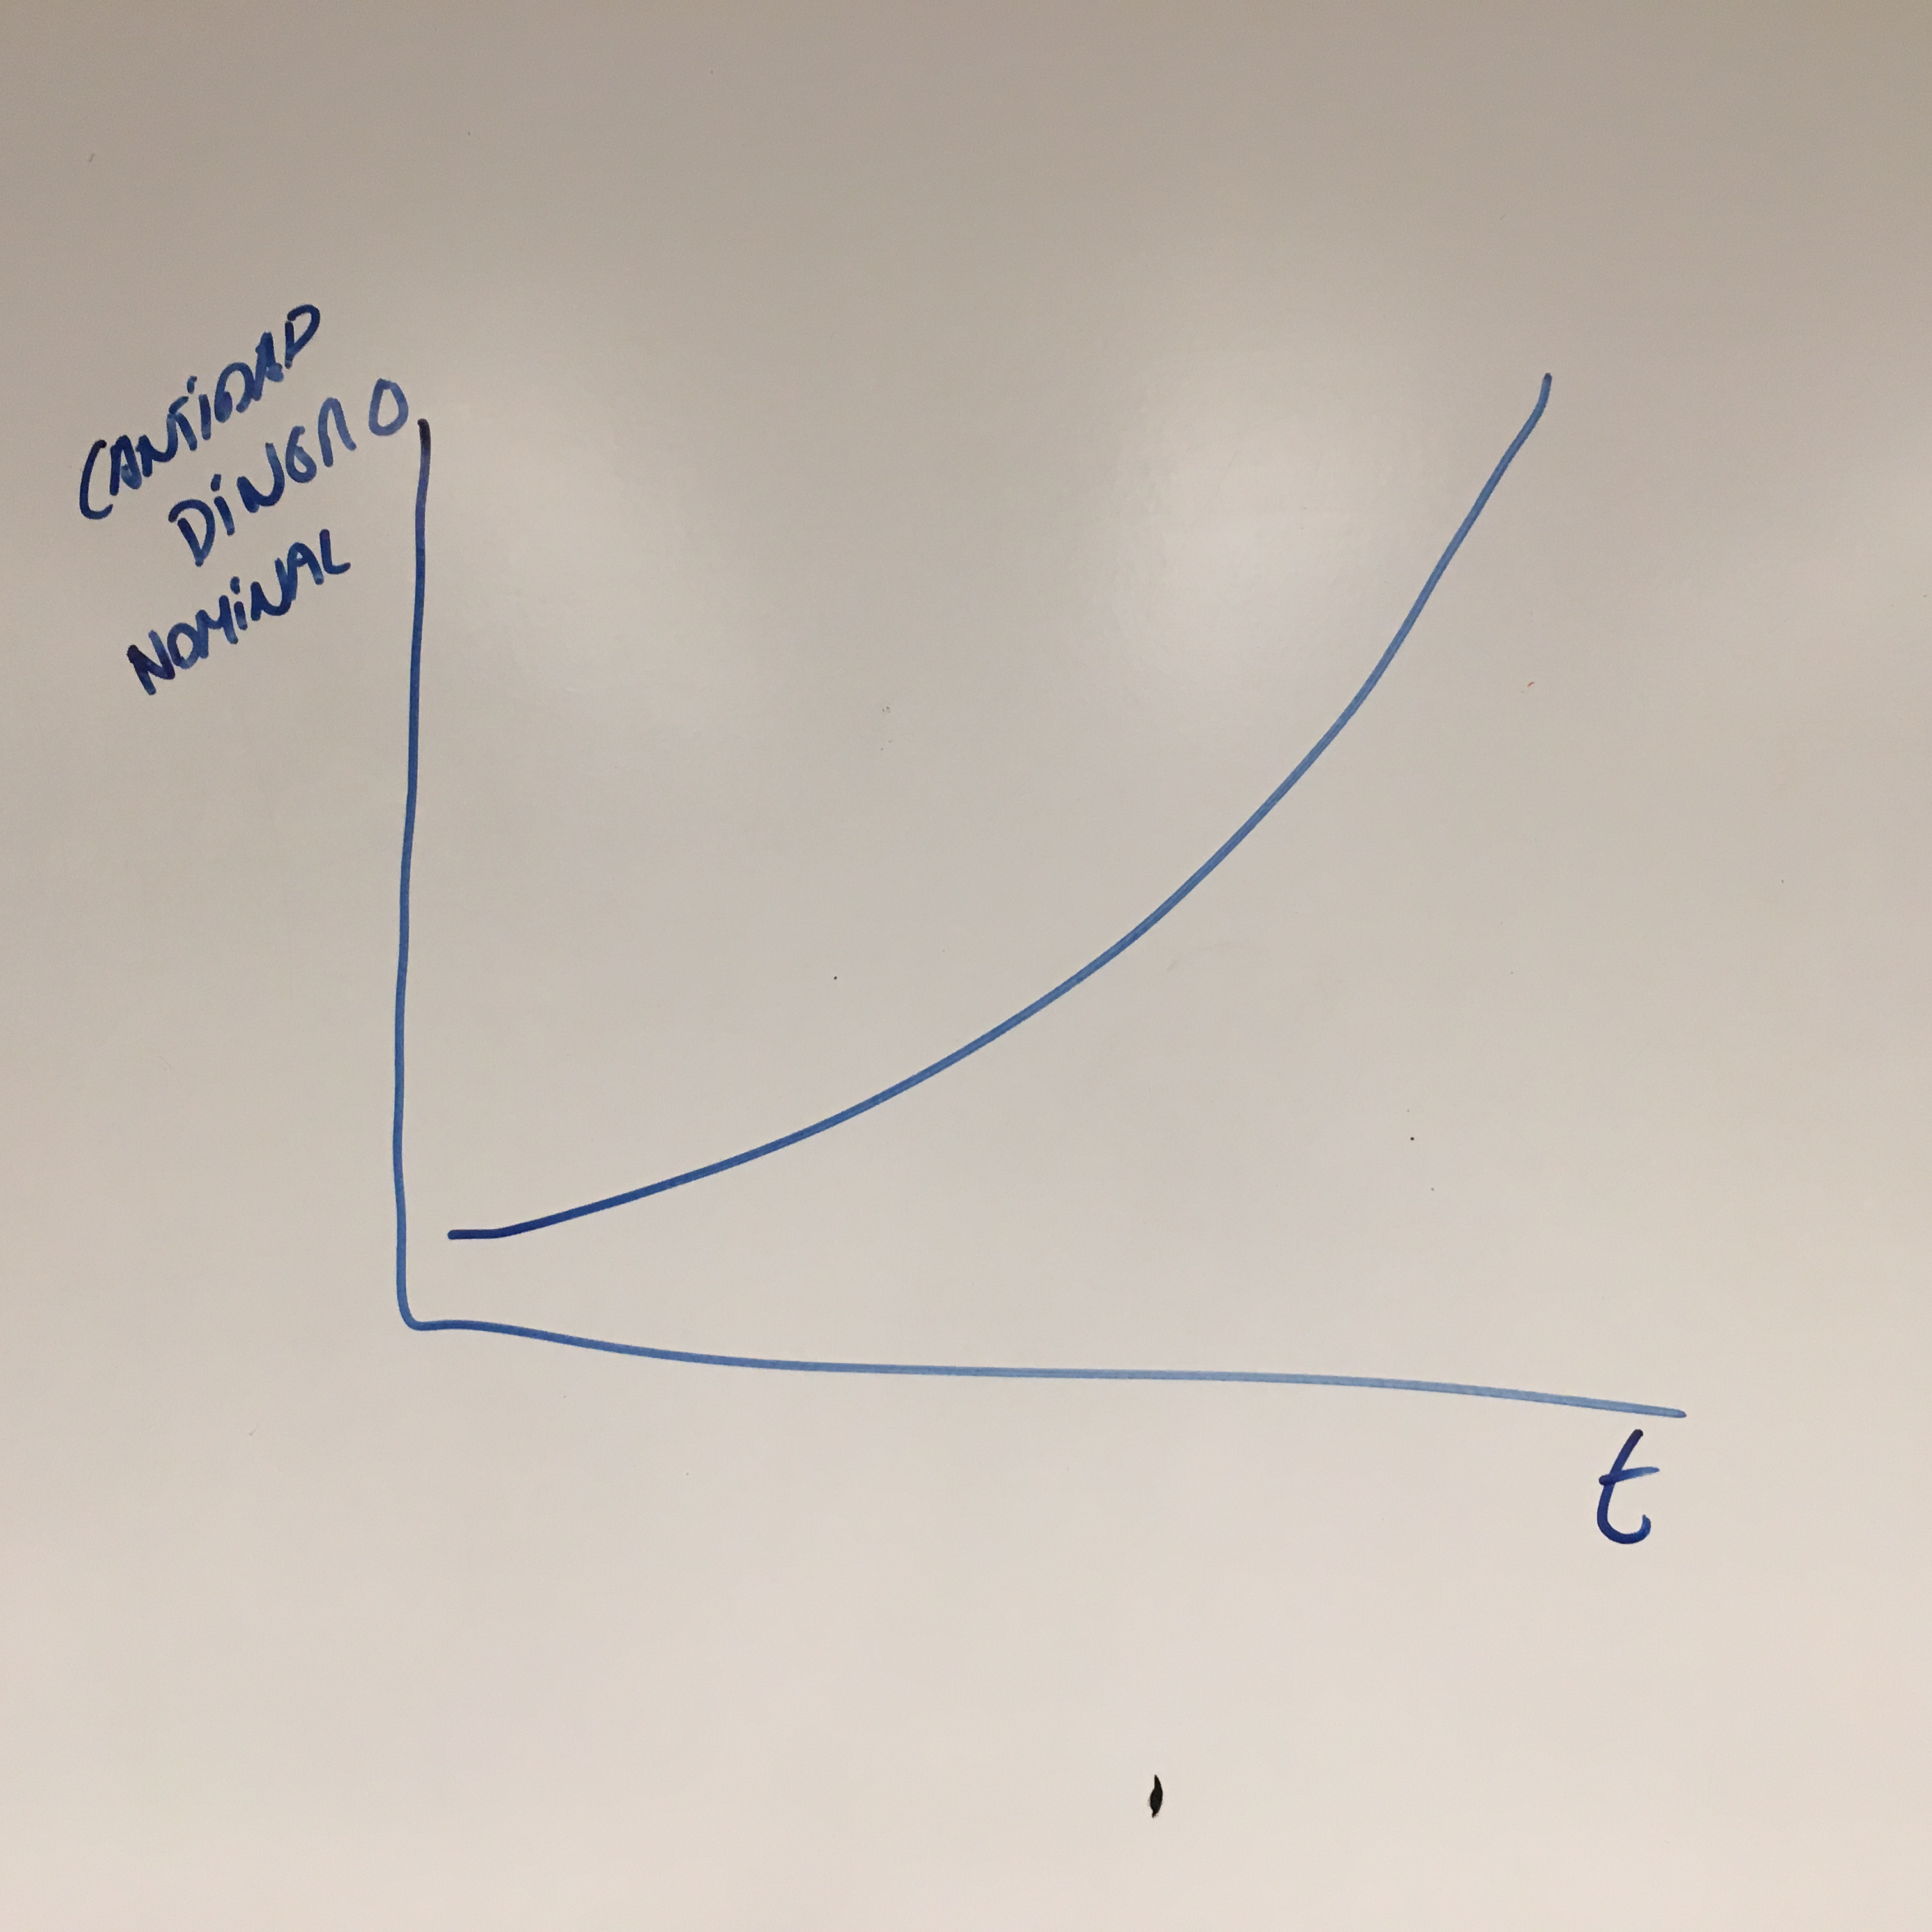
\includegraphics[width=6cm]{Classes/Images/2019-10-09_1.JPG}
                    \caption{El eje-x es tiempo, y el eje-y es la cantidad nominal de dinero}
                    \label{}
                \end{figure} 
                \begin{figure}[htbp]
                    \centering
                    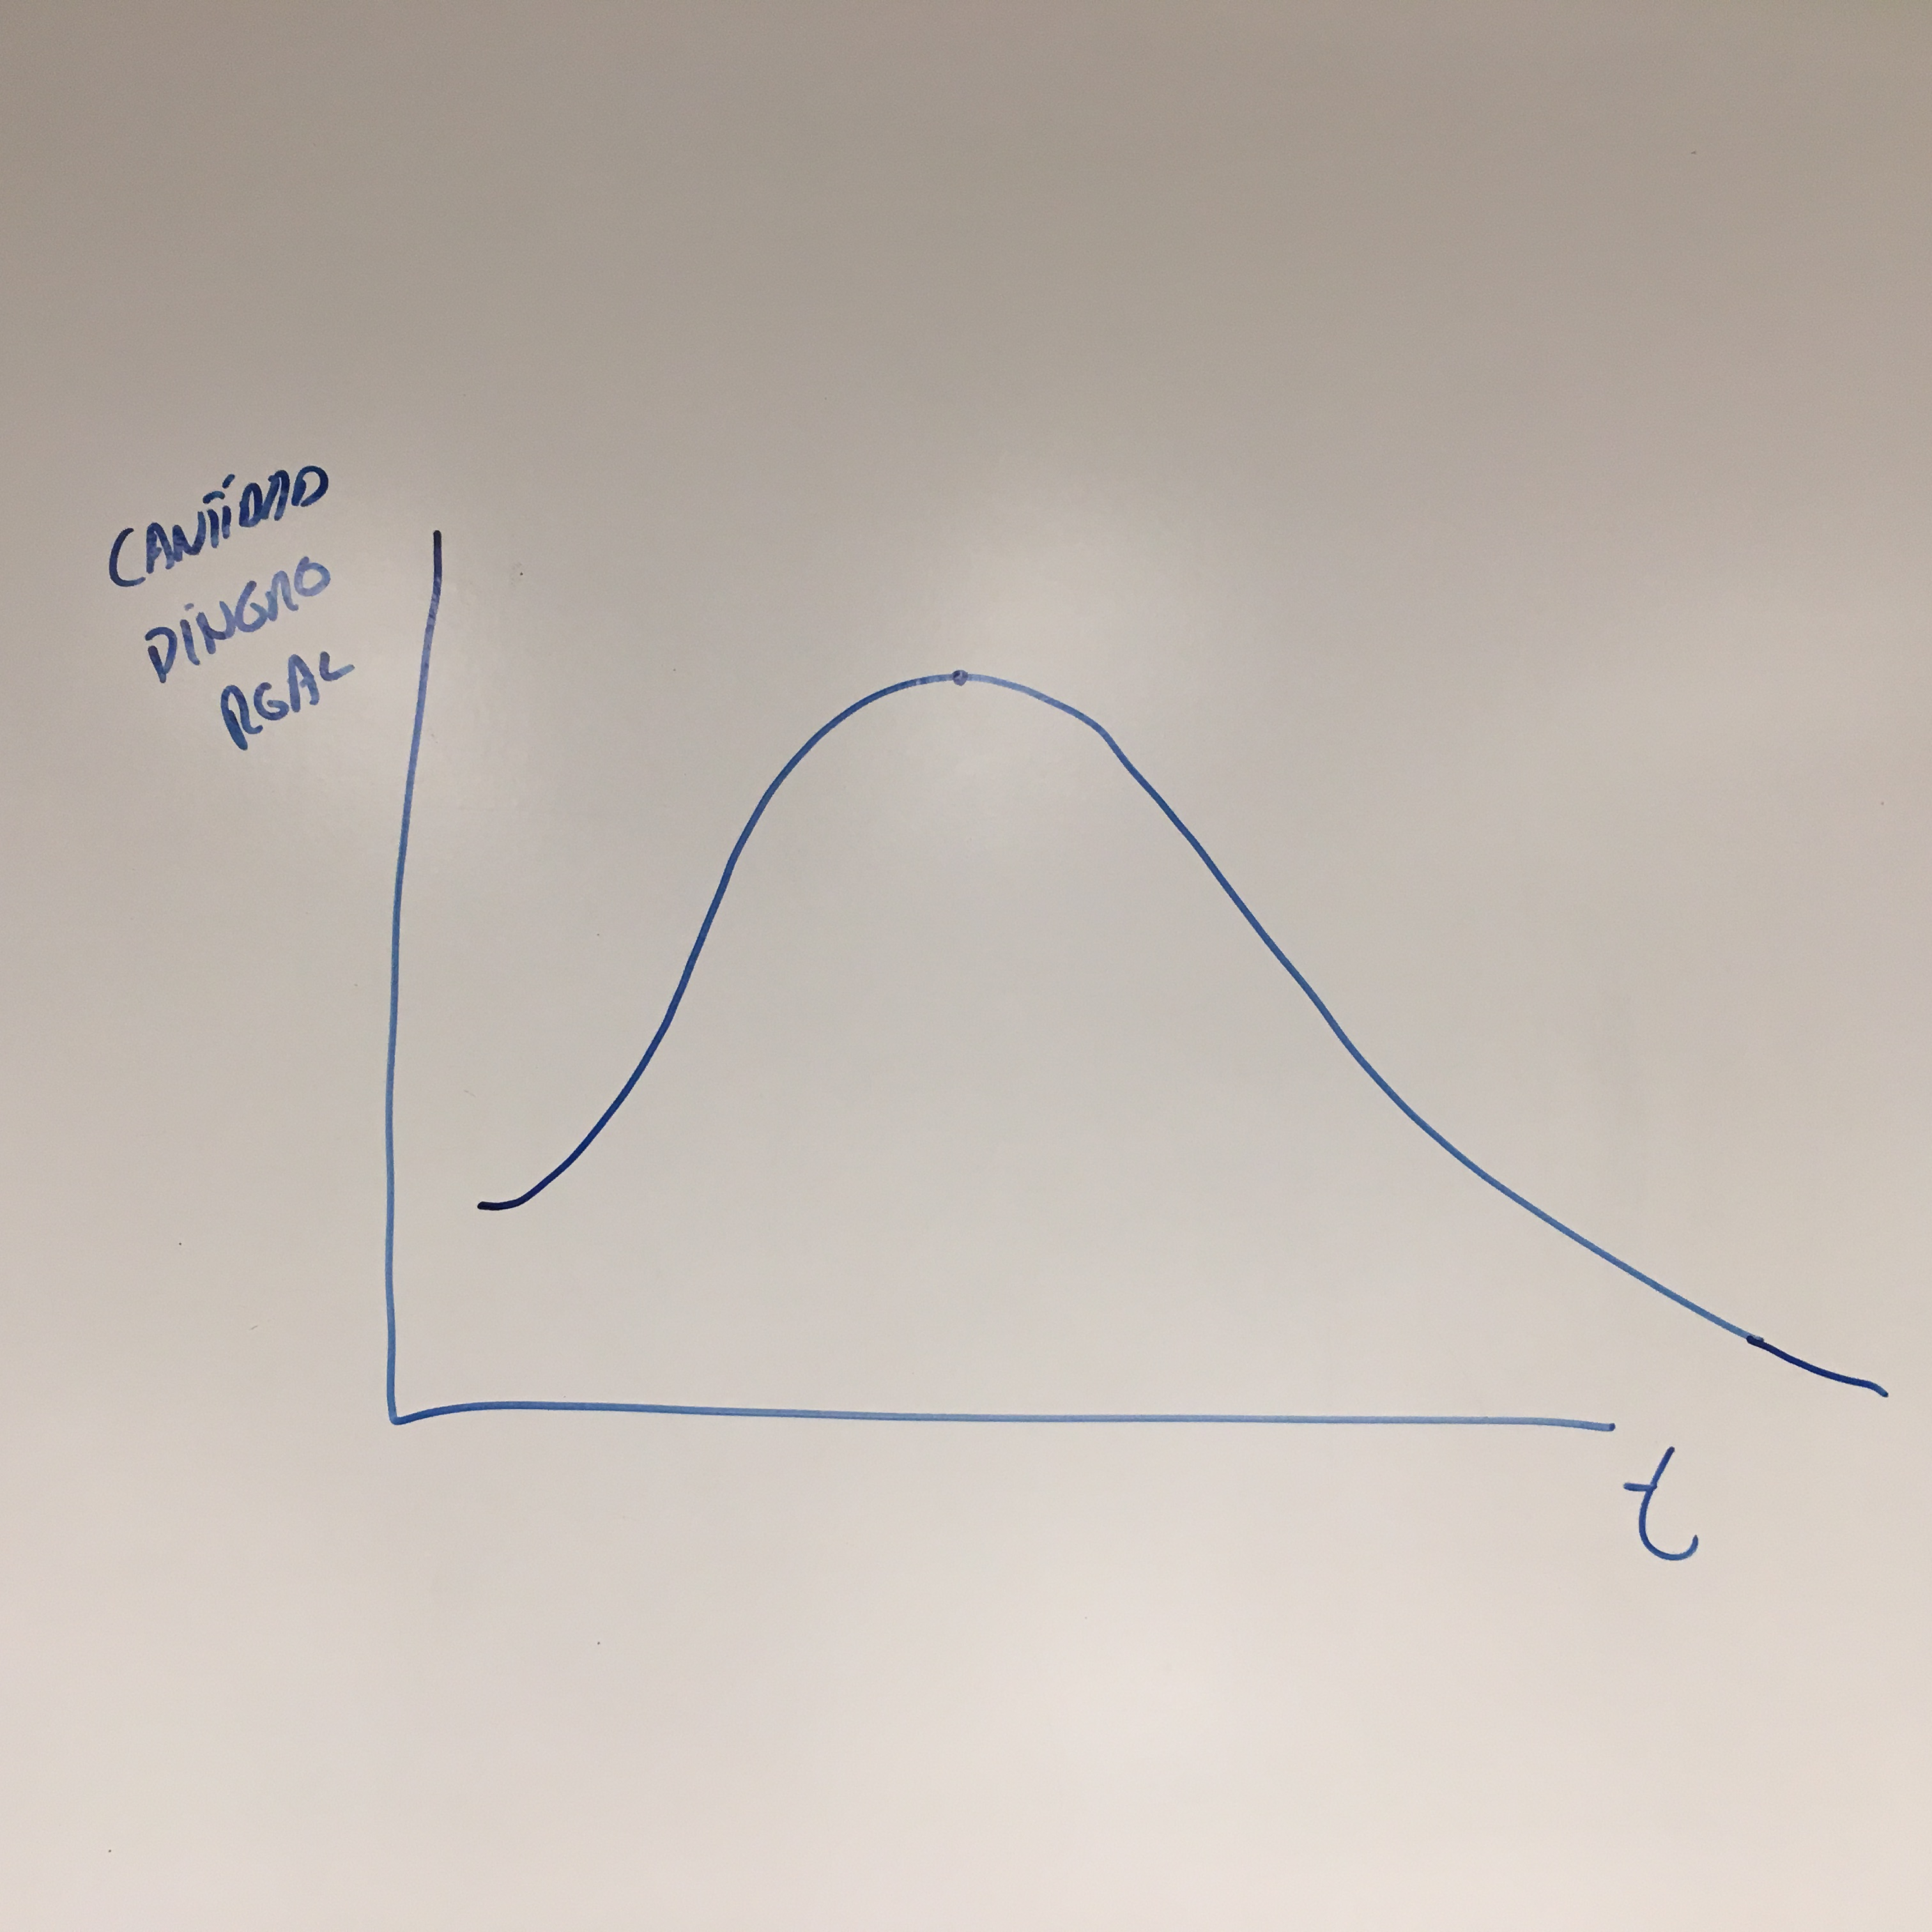
\includegraphics[width=6cm]{Classes/Images/2019-10-09_2.JPG}
                    \caption{El eje-x es tiempo, y el eje-y es la cantidad de dinero real}
                    \label{}
                \end{figure} 
            
            \item Considerar la siguiente fórmula para calcular:
                \[
                  \text{Oferta de dinero real} = \frac{\text{Oferta nominal}}{\text{Precios}}
                \]
            
            \item La demanda de dinero depende de la incertidumbre, cuando se siente que se va a depreciar la moneda todas las personas se quieren deshacer de la moneda por que los voy a perder, por eso se dice que la que tiende a circular la \textbf{buena moneda}. Considerar lo siguiente, en las hiper-inflaciones es de cobrar más amenudo \emph{\textbf{Ejemplo: }te cobran cada 15 minutos.}
            \item El punto de quiebre es cuando todos anticipan la depreciación de la moneda entonces se produce una escazes de dinero. 
        \end{itemize}
        
        \item Entonces el dinero es tan disfuncional que se vuelve a un trueque, se \textbf{rechaza} la moneda por completo. Se tiende a observar cosas como el barendero barriendo miles de millones en la divisa hiper-inflada por que es más valioso el papel que está hecho el dinero que el dinero en sí.
        \item \emph{\textbf{Ejemplo: }Venezuela y el precio del www.dollartoday.com es un sitio que se utiliza para averiguar el valor actual en Bolívares}.
        \item La ley de Thiers va a aplicar cuando la oferta de moneda sea mucho y pierde su función de medio de intercambio generalmente aceptado, en este momento se cumple la ley de Thiers por que ya no vale nada.
        \item \emph{Citación:``Siempre cuando exceda el punto de quiebe y la oferta del dinero real va en picada se aplica la ley de Thiers."}
        \item \emph{Citación:``Antes de la hiper-inflación iba con un poco de dinero y podía comprar una carreta de bienes, ahora voy con una carreta de dinero y regreso con un solo bien"}
        \item \emph{\textbf{Definición de ``punto de quiebre":} cuando el denominador  osea los precios son más grandes que la oferta real de dinero}
        \item Se puede hacer algo para revertir una hiperinflación si el gobierno se compromete se deprecian los precios, para hacer eso hay que  dejar de hacer déficit fiscal.
        \item \emph{\textbf{Ejemplo: }Venezuela no se dollariza por razones de nacionalismo}
        \item Dos indoles:
            \begin{enumerate}
                \item Índole 
                \item Índole bélica, cuando hay guerra siempre habrá un déficit fiscal, la salida o la forma de mobilizar grandes cantidades de recursos es aumentar la cantidad de dinero.
            \end{enumerate}
        
        \item \emph{\textbf{(Paréntesis ``paris como un foco de ideología'':}Siempre las ideas socialistas y de izquierda surgen de París  \textbf{)}} \emph{\textbf{Recordar lo siguiente:}Jermenes rojos, cuando juzgan este régimen ponen de escusas su adoctrinación en París de sus profesores marxistas.}
        \item \emph{Citación:``El camino al infierno está plagado de buenas intenciones"}
        \item En el manifiesto communista establece que para instituir un régimen socialista se debe de hacer hiper-inflación para quitarle todo el valor al dinero. 
        \item \emph{\textbf{Ejemplo: }hiper-inflación de beimar}
        \item Causas de una hiper-inflación: 
            \begin{enumerate}
                \item Ignorancia
                \item Socialismo o comunismo
            \end{enumerate}
        
        \item GT es un país estable por que el gobierno no tiene control en el banco central.
\end{enumerate}


\chapter{2019-10-14}
\section{Resolución de corto}   
\begin{enumerate}
    \item Para qué sirve tener saldos de caja: para la incertidumbre
    \item Por que la inflación hace que los pobres sean más pobres:  que ellos tienen más saldos de caja.
    \item La ley de Gresham tiene un tipo de cambio establecido, y hace circular la mala moneda.
    \item La ley de Thiers aplica con la hiperinflación, los tres pasos y el punto de quiebre.
\end{enumerate}

\section{Noticia \textbf{Nos preguntamos:} ¿Why socialism stinks?}
\begin{enumerate}
    \item Robert Lawson, 
    \item Argumento de Swesia, por los tipos de pseudo-socialismo.
    \item Los empresarios empezaron a huir de las pol+iticas socialistas y Swesia bajó los impuestos.
    \item Cuba: 
    \begin{itemize}
        \item Opresión, persecución, espionaje 
        \item Las famosas etapas del socialismo ``real'':      
        \item Hoteles: inicialmente los turistas se quedarían en hoteles y propagar las ideas socialistas, pero ahora los hoteles están mal.
    \end{itemize}

    \item En las drogas illegales uno no puede quejarse por la calidad del producto, las drogas legales sí se puede alegar la calidad.
    \item Muertes atribuidas al socialismo:
        \begin{itemize}
            \item Mao Zedong
            \item Stalin 
            \item Holocausto
        \end{itemize}
    \item Ver: Holodomor, URRS Rusia con mano de hierro con un montón de repúblicas satélites, el telón de acero (división de europa en la que una mitad es socialista y otra es capitalista). \emph{\textbf{Observación: }Ukrania recibió con los brazos abiertos a los nazis}, \emph{\textbf{Recordar lo siguiente: }Cuando se intentó industrializar la repúblicas agrarias y nadie se queda produciendo la comida y todos se mueren de hambre.}
\end{enumerate}

%%%%%%%%%%%%%%%%%%%%%%%%%%%%%%%%%%%%%%%%%%%%%%%%%%%%%%%%%%%%%%%%%%%%%%%%%%%%%%%%%%%%%%%%%%%%%%%%
\section{Discusión de noticia \& de clase}
\begin{enumerate}
    \item Ben Powel, su investigación de ir a regímenes socialistas y conversar con las personas en los bares.
    \item \textbf{Nos preguntamos:} ¿Por qué la taza de mortalidad de los infantes es tan buena en los países socialistas? \emph{\textbf{La respuesta a esta pregunta es: }Cómo se modifica las cifras del estado, \emph{\textbf{Recordar lo siguiente: }el Correismo, es el siglo del sigo XXI, sostiene el objetivo de nacionalizar a los medios de producción, es la versión latinoamericana del socialismo, se tiende a preferir la adquisición del poder por medios democráticos.}}, lo que hicieron en Ecuador, querían aumentar la alfabetización entonces pusieron a los que estaban saliendo del colegio en lugar de hacer seminario se le ponía a alfabetizar a todos los demás, pero esto solo eran cifras no se alfabetizo casi nada. 
    \begin{itemize}
        \item Las autoridades cubanas se manipulan mucho las cifras ya que los índices de mortalidad infantil de Cuba se entendió que tiraban todas las muertes infantiles las catalogan como muertes en el vientre, y no como muertes infantiles por ende las cifras de mortalidad infantil subió exponencialmente aparentando que el socialismo de cuba esté funcionando.
    \end{itemize}
    Tres pilares de los indices de desarrollo humano: 
    \begin{enumerate}
        \item Renta
        \item Educación 
        \item Sanidad
    \end{enumerate}
\end{enumerate}

\subsection{Menger y su evolución de dinero}
\begin{enumerate}
    \item Menger dice que nadie se inventó el dinero ha surgido espontáneamente, este es fruto de el humano pero no es diseñado por un humano, \emph{\textbf{Ejemplo: }el español surgió inicialmente por personas que hablaban mal el latín, los lenguajes se desarrollan con las sociedades de personas}.
    \item \textbf{Nos preguntamos:} ¿Lenguajes diseñados? \emph{\textbf{La respuesta a esta pregunta es: }existió uno llamado ``esperanto'' que se intentó universalizar el lenguaje con este nuevo lenguaje, pero fracasó por que nadie lo hablaba, se intento para evitar guerras, el esperanto está muerto.} \emph{\textbf{Ejemplo: }Otro ejemplo es el hebreo}.
    \item Utilizar la analogía del lenguaje para entender el surgimiento del dinero, surge \textbf{espontáneamente}.
    \item \textbf{Nos preguntamos:} ¿Proceso de creación del dinero? \emph{\textbf{La respuesta a esta pregunta es: }El proceso de economía trival es increiblemente costoso, el \emph{Citación:``el trueque directo es mucho más indirecto que el trueque indirecto"} }, \emph{\textbf{Observación: }es mucho más probable ver más intercambios en una economía de trueque que en una economía con dinero, \emph{\textbf{Ejemplo: }quiero un reloj $\Rightarrow$ cambio algo $\Rightarrow$ cambio algo $\Rightarrow$ cambio algo $\Rightarrow$ llego a tener un reloj}}.
    \item \emph{\textbf{Observación: }Economías trivales: el trueque}
    \item Hay bienes que se venden fácil y otros que no, hay bienes que por alguna razón tiene una demanda mayor a la otros.
    \item \textbf{Nos preguntamos:} ¿Qué hago para hacer trueque en una economía de dinero? ver el bien que es más demandado y y buscar usarlo como unidad de cuenta, entonces el trueque se disminuye ya que puedo poner lo que quiero intercambiar por el equivalente en ese bien vendible, surge una \emph{una demanda monetaria.}, esto \textbf{incrementa la capacidad de intercambio.} Por eso en diferentes civilizaciones usaban diferentes dineros \emph{\textbf{Ejemplo: }en centroamérica la gente usaba cacao por su vendibilidad pero lo terminaron ya no utilizando por que es perecedero.}
    \item Cuando surge un dinero que sobre sale sobre el resto, es cuando hablamos de dinero, se desarrolla una demanda monetaria y todo se empieza a medir por ese bien altamente vendible.
    \item \textbf{Nos preguntamos:} ¿El estado y la legislación en relación al dinero? \emph{\textbf{La respuesta a esta pregunta es: }El estado no crea el dinero, solo pone un sello que garantiza calidad y cantidad, pero el dinero es selecciónado espontáneamente.}, \emph{\textbf{Observación: }Lydia es una de las civilizaciones que en el siglo VII antes de Cristo en emitir una moneda, \textbf{Nos preguntamos:} ¿por que se pone un borde y un sello en la moneda? \emph{\textbf{La respuesta a esta pregunta es: }asegura la calidad de la moneda, Es un desarrollo reciente que garantiza cantidad y calidad del dinero, pero no es dinero por el sello.}}
    \item \emph{\textbf{(Paréntesis ``dinero fiat'':}era un dinero que era básicamente pasivos, es dinero que se basa en la confianza fiat viene del latín que significa confianza, es dinero fiduciario.\textbf{)}}
    \item \emph{\textbf{Observación: }El amazon giftcard es dinero en la comunidad de amazon, el store credit es un tipo de dinero (generalemente aceptado) en la comunidad de walmart}
    \item \emph{\textbf{Ejemplo: }Bitcoin, los gobiernos más bestias los quieren prohibir}
\end{enumerate}

\subsection{Parcial el lunes 28}




\chapter{2019-10-16}
\section{Noticia de el crecimiento económico de un país en relación con el banco central}
\begin{enumerate}
    \item La economía en aumento no signifique que la banca deba meterse para asegurarse que no se inflen los precios.  
\end{enumerate} %pib irreal o real

%%%%%%%%%%%%%%%%%%%%%%%%%%%%%%%%%%%%%%%%%%%%%%%%%%%%%%%%%%%%%%%%%%%%%%%%%%%%%%%%%%%%%%%%%%%%%%%%

\section{Análisis de noticia}
\begin{enumerate}
    \item Análisis:
        \begin{itemize}
            \item $M_{\text{Cantidad de dinero}} \leftarrow Q_{\text{Cantidad de bienes}}$ 
        \end{itemize}
\end{enumerate}

\section{Discusión de clase}
\begin{enumerate}
    \item John locke: \emph{Citación:``Como tienen un interés bajo son ricos y por que tenemos interés alto somos pobres"}, un principio al pensamiento económico, el tipo de interés bajo es un efecto del desarrollo económico no es la causa del pensamiento económico.
    \item \emph{\textbf{Recordar lo siguiente: }La base del desarrollo económico es la inversión y para invertir necesito ahorrar, Holanda tenía un tipo de interés bajo porque tenía ahorros, inversión, etc.}
        \begin{center}
        \begin{tabular}{ | p{5cm} | p{5cm} | }
         \hline
        \multicolumn{2}{|c|}{Banco X} \\
        \hline  
        $+\underbrace{\text{Préstamo}}_{\text{Activo del banco}}$ & $+\underbrace{\text{Depósitos}}^{\text{Pasivos del banco}}$ \\ 
         \hline
        \end{tabular}
        \end{center}
    
    \item El banco es básicamente un comerciante de crédito. Intereseante: Con los préstamos incrementa los depósitos. 
        \begin{itemize}
            \item Los cheques son equivalentes a los pagos por tarjeta de débito.
            \item Cuando tu le pagas al banco mediante un depósito se va cancelando el préstamo que adquiriste.
            \item \textbf{La cantidad de bienes} incrementa la cantidad de dinero.  
        \end{itemize}
\end{enumerate}

%%%%%%%%%%%%%%%%%%%%%%%%%%%%%%%%%%%%%%%%%%%%%%%%%%%%%%%%%%%%%%%%%%%%%%%%%%%%%%%%%%%%%%%%%%%%%%%%
\subsection{Cálculo del PIB nominal \& PIB Real}

\[
  \Delta PIB_{\text{Nominal}} = \frac{P_{1}*P_{1}}{\underbrace{P_{0}}_{\text{¿$\Delta p$?}}* \underbrace{q_{0}}_{\text{¿$\Delta q$?}}} \approx 1'08 = 8\% \\ 
  \text{Donde P es precios y q es cantidad}
\]

\[
    \Delta PIB_{\text{Real}} = \frac{P_{0}*q_{1}}{P_{0}*q_{0}} \approx 1'03 = 3\% \\ 
    \text{Donde P es precios y q es cantidad}
\]

Los Datos deben de ser el PIB real no el nominal, en el nominal tiene el efecto precio  




%%%%%%%%%%%%%%%%%%%%%%%%%%%%%%%%%%%%%%%%%%%%%%%%%%%%%%%%%%%%%%%%%%%%%%%%%%%%%%%%%%%%%%%%%%%%%%%%
\subsection{Historia, cómo llegamos del oro a la moneda moderna}
\begin{enumerate}
    \item \emph{\textbf{Recordar lo siguiente: }Cómo se seleccionan los dineros en el bimetalismo, se establece un ratio o tipo de cambio fijo y se genera la ley de Gresham, el camino al infierno está lleno de buenas intensiones}.
    \item Cuando se establecían esos tipos de cambio fijo se tendía a infravalorar y sobrevalorar el otro dinero, es decir que el tipo de cambio no reflejaba el valor real de la moneda.
    \item Se dice que el mundo se pasa casi completamente en el siglo 19 al patrón oro, Inglaterra ya estaba en el patrón oro.
    \item Interesante: Newton, \emph{\textbf{(Paréntesis:} La física de newton\textbf{)}}, \emph{\textbf{(Paréntesis ``uno de los ultimos hombres del renacimiento'':}significa que sabía un poco de todo, por eso se la da el nombre de universidad.\textbf{)}}, Newton ejercía el rol de la ceca \emph{\textbf{Definición de ``ceca":} es un nombre común denominado a un objeto}, Newton establece un precio del oro y de la plata para intentar dejar a Inglaterra en el patrón oro, pero no circuló el oro si otra moneda \textbf{los bancos}. 
    \item Los bancos ya existían en el siglo XVIII.
    \item Entonces tenían el patrón oro es peligroso por el oro, guardarlo en la casa era peligroso también, entonces la gente le empieza a dejar su dinero a especialistas a estos denominados primeros banqueros, estos primeros banqueros eran los goldsmiths ellos tenían ya metales preciosos y ya tenían la especialidad de cuidar esos metales preciosos.
    \item Los goldsmiths les daban a los depositantes papel moneda estableciendo un pagaré.
    \item Entonces empiezan a circular \textbf{Los pagarés del orfebre o los pagarés}, entonces tenemos un patrón oro donde no circula el oro si no billetes de pagarés del orfebre ó papel moneda.
    \item Empieza a surgir el banco central de Inglaterra, empieza intercambiar un papel, entonces le dio \textbf{la característica de transportabilidad al oro.}
\end{enumerate}


\chapter{2019-10-18}
\section{Recomendaciones}
\begin{enumerate}
    \item   
\end{enumerate}
%%%%%%%%%%%%%%%%%%%%%%%%%%%%%%%%%%%%%%%%%%%%%%%%%%%%%%%%%%%%%%%%%%%%%%%%%%%%%%%%%%%%%%%%%%%%%%%%

\section{Video de VisualPolitik}
México y su crecimiento económico:
\begin{enumerate}
    \item López Obrador, referéndum \% de aprobación por causas muy atractivas, cancela la construcción de el aeropuerto internacional de México.
    \item La inversión política en México está en picada por la razón que López Obrador cancela grandes proyectos como el de AIM.
    \item Después de una enfermedad holandesa es decir: recursos nacionalizados $\Rightarrow$ privatizar los recursos, es muy difícil.
    \item PeMEX, un recurso nacionalizado, es difícil privatizar algo que no funciona en el sector pública.
    \item Problema de el sector de educación con el sindicato; un problema de privilegios entre los sindicatos educativos.
    \item Medida de ley que el ejercito puede combatir el narco-tráfico, el problema es que todo cambio para seguir exactamente igual.
    \item El problema del tren Maya, por problemas económicos.
    \item Problemas económicos:
        \begin{itemize}
            \item El problema es que el rule of law es muy cambiante.
            \item También que se paró la construcción y limitó la inversión extranjera.
        \end{itemize}
\end{enumerate}
%%%%%%%%%%%%%%%%%%%%%%%%%%%%%%%%%%%%%%%%%%%%%%%%%%%%%%%%%%%%%%%%%%%%%%%%%%%%%%%%%%%%%%%%%%%%%%%%
\section{Video de Oscar Alejandro El malecón, 12 cosas impresionante de Cuba}
\begin{enumerate}
    \item Puesto \# 12: 
        \begin{itemize}
            \item No hay publicidad.
            \item No hay marcas.
            \item No existen las marcas ni los tipos de productos, lo únicos anuncios son propaganda del dinero.
        \end{itemize}

    \item Los hombres se besan en el cachete: 
        \begin{itemize}
            \item Asunto de cultura.
        \end{itemize}
    
    \item Existen dos monedas nacionales:
        \begin{itemize}
            \item El peso convertible (supuestamente, un peso convertible = un dollar).
            \item Existe el billete de tres pesos convertible.
        \end{itemize}
    
    \item No existen los puestos de venta:
        \begin{itemize}
            \item Ninguno de estos sistema existe en Cuba. 
            \item Hay que traer dinero en efectivo.
            \item No funcionan las tarjetas MasterCard ni Visa.
        \end{itemize}
    
    \item Tratan mejor al turista que al cubano: 
        \begin{itemize}
            \item No se le dan buen trato al cubano.
            \item Está prohibido andar sin camisas.
            \item Si sos turista no importa.
        \end{itemize}
    
    \item Casas y carros viejos:
        \begin{itemize}
            \item Son antigüedades que se mantienen solas.
        \end{itemize}
    
    \item Tarjetas de internet: 
        \begin{itemize}
            \item Se necesita comprar tarjetas para acceder al internet, son básicamente datos, para los cubanos esto insostenible.
            \item nauta, tipo de tarjeta.
        \end{itemize}
    
    \item El paquete semanal: 
        \begin{itemize}
            \item Sistema para poder estar conectado sin internet, es un discoduro que tiene todas las películas de YouTube, netflix etc.
            \item Los videos que se encuentran ahí las escogen los que distribuyen.
        \end{itemize}
    
    \item Salario mínimo: 
        \begin{itemize}
            \item De 20\$ al mes, no alcanza para nada, esta es la fuente de la pobreza.
        \end{itemize}
    
    \item La libreta de racionamiento: 
        \begin{itemize}
            \item Son subsidios por los productos.
            \item Es un instrumento de control político, por que se puede controlar.
            \item La gente piensa que es mejor pero no.
        \end{itemize}
    
    \item La seguridad: 
        \begin{itemize}
            \item No existe la inseguridad.
            \item Cometer un crimen o robo es anti-revolucionario.
            \item Esto es algo bueno.
        \end{itemize}
    
    \item El cubano siempre está feliz: 
        \begin{itemize}
            \item La actitud del cubano es muy buena.
            \item Pero la mayoría de gente está mal y ha cedido a las cosa estar así de mal en Cuba.
            \item Ya perdieron la esperanza del cambio.
            \item \textbf{Nos preguntamos:} ¿Por qué ir a cuba solo para ayudar el régimen? \emph{\textbf{La respuesta a esta pregunta es: }Ayudar a la gente pero está el trade-of de ayudar por medio de impuestos.}
        \end{itemize}
\end{enumerate}

%%%%%%%%%%%%%%%%%%%%%%%%%%%%%%%%%%%%%%%%%%%%%%%%%%%%%%%%%%%%%%%%%%%%%%%%%%%%%%%%%%%%%%%%%%%%%%%%
\section{Video de VisualPolik, Silicon Valley es tan rico}
\begin{enumerate}
    \item Es en California donde está la tercera zona más grande del mundo: 
        \begin{itemize}
            \item No tienen minas de silicio ni ningún recurso natural.
            \item Tiene la tasa de impuestos más alta de EEUU.
            \item \textbf{Nos preguntamos:} ¿Con estas tasas de impuestos cómo es uno de los estados más ricos?
            \item Historia:
                \begin{itemize}
                    \item Shockley, una fábrica de semiconductores basados en silicio.
                    \item Los ocho traidores, se revelan e intentan hacer su propia empresa.
                    \item En 1959, nació la empresa de fondo capital riesgo (ahorros de personas que están dispuestas a arriesgar su dinero).
                    \item El valor de una idea: después de la II guerra mundial, todos regresan a casa y querían emprender, entonces se empieza a demandar el fondo de capital riesgo.
                    \item Rockfeller y sus amigos millonarios financian la idea de los ocho traidores.
                    \item En este proceso nacen el primer fondo de capital riesgo.
                    \item Surge Fairchild semiconductors.
                    \item La clave de esta riqueza es porque lograron por medio de fondos de capital riesgo atraer los ahorros de todo el mundo.
                \end{itemize}
            
            \item El método Silicon Valley: 
                \begin{itemize}
                    \item IKEA, sólo crecía con sus propios fondos.
                    \item Facebook, es un negocio escalable, no importa la cantidad de clientes sus gastos son básicamente los mismos.
                    \item Esto es la clave del funcionamiento de Silicon Valley.
                \end{itemize}
            
            \item Clave: 
                \begin{enumerate}
                    \item El valle de la muerte.
                    \item Convertirse en una empresa.
                    \item Buscar un business angel, una persona dispuesto a invertir en una empresa en el valle de la muerte. $\equiv$ Peter Teal.
                        \begin{itemize}
                            \item El business angel compite con otros business angels.
                            \item Se tratan de competir por la inversión en empresas en el valle de la muerte.
                        \end{itemize} 
                    \item Start-up $\Rightarrow$ crecer, por ende se acude a un fondo de capital riesgo.
                        \begin{itemize}
                            \item En 2005, se hace un fondo de capital de Palmers. 
                            \item Entonces Facebook's Peter Teal, su medio millón de dolares se convirtieron en 15 millones.
                            \item Apple compra Shazam por ejemplo. 
                        \end{itemize}
                \end{enumerate}
            
            \item \textbf{Nos preguntamos:} ¿Se puede replicar el método silicon valley en otros países?
        \end{itemize}
\end{enumerate}


\chapter{2019-10-23}
\section{Resolución de corto}
\begin{enumerate}
    \item \textbf{Nos preguntamos:} ¿Por qué en holanda había un tipo de interés bajo que en Inglaterra? \emph{\textbf{La respuesta a esta pregunta es: }porque había más ahorro, más inversión.}
    \item \textbf{Nos preguntamos:} ¿Cuál es la base de todo crecimiento económico? \emph{\textbf{La respuesta a esta pregunta es: }ahorro} 
    \item \textbf{Nos preguntamos:} ¿Por qué el orfebre se convirtió en el primer banquero? \emph{\textbf{La respuesta a esta pregunta es: }por que era el especialista, era peligroso y costoso guardar el oro.}
\end{enumerate}

%%%%%%%%%%%%%%%%%%%%%%%%%%%%%%%%%%%%%%%%%%%%%%%%%%%%%%%%%%%%%%%%%%%%%%%%%%%%%%%%%%%%%%%%%%%%%%%%
\section{Noticia Health care insurance, discusión análisis}
\begin{enumerate}
    \item Single payer tax health care, sostiene la propuestas que todos los gastos en salud el gobierno iba a asegurar por medio de impuestos, totalmente financiado por el gobierno.
    \item Esto elimina la competencia y fomenta un ambiente atractivo para un monopolio.
    \item Definen la ``salud esencial'' como la salud mental no es esencial y no lo cubre el gobierno.
    \item Single payer system vs multi-payer system.
    \item Elimina los incentivos para hacer las cosas mejor ya que el gobierno siempre te pagará aun que hagas un producto basura.
\end{enumerate}
%%%%%%%%%%%%%%%%%%%%%%%%%%%%%%%%%%%%%%%%%%%%%%%%%%%%%%%%%%%%%%%%%%%%%%%%%%%%%%%%%%%%%%%%%%%%%%%%
\subsection{Análisis de noticia}
\begin{enumerate}
    \item Sistema Bismac, Bebeich; es el primero que instituye el sistema de salud de Alemania.
    \item Curiosamente, en EEUU McDonald's tenía un mejor plan de sanidad que ObamaCare.
    \item \emph{\textbf{Interesante:} El asunto en EEUU los empresarios deciden proveer a sus empleados por que es un deducible de los impuestos.}
    \item \emph{\textbf{Interesante:} EEUU es uno de los países que hay un exceso en los costos de prevención de enfermedades, todos los que ObamaCare .}
\end{enumerate}

%%%%%%%%%%%%%%%%%%%%%%%%%%%%%%%%%%%%%%%%%%%%%%%%%%%%%%%%%%%%%%%%%%%%%%%%%%%%%%%%%%%%%%%%%%%%%%%%
\section{Discusión de clase}
\begin{enumerate}
    \item El sistema americano, no es plenamente privado, subcidia la demanda, la oferta es libre, subsidia la demanda mediante impuestos, \textbf{\emph{El problema es este: que la oferta no está restringido entonces es gratis ir hasta de broma al médico.}} Por eso EEUU gasta hasta el 18\% del PIB en sanidad, el que más gasta en sanidad en el mundo, el siguiente es Cuba.
    \item $\Rightarrow$ Subcidio de demanda $\Rightarrow$ La oferta puede 
    \item Beverich: 
        \begin{itemize}
            \item Single payer, en Europa lo que ocurre es que la demanda se \textbf{queda fija}, entonces se forman listas de espera.
            \item Con un tope hacen que si tu queres ir al médico tenes que esperar.
            \item En España Daniel se había estropeado la rodilla y se logró curar antes de ver un médico.
            \item El estado define cuánto podes gastar.
        \end{itemize}
    
    \item Bismarck: 
        \begin{itemize}
            \item Te obliga a tener seguro, 
            \item \emph{\textbf{Interesante:} En Singapur te dicen, ``el 15\% de tu sueldo va a ahorrar'', esto funciona por que a pesar que es un poco paternalita, esto soluciona por que hay menos incentivos a no ir al médico solo por la gana de ir. este es el sistema más privado que existe.}
            \item \textbf{Nos preguntamos:} ¿Tiene sentido asegurarme en contra de la gripe? No, uno se asegura en contra de eventos de riesgo parametrizable.
            \item En conclusión el sistema de salud Bismack es más bueno en términos de sanidad.
        \end{itemize}
\end{enumerate}

%%%%%%%%%%%%%%%%%%%%%%%%%%%%%%%%%%%%%%%%%%%%%%%%%%%%%%%%%%%%%%%%%%%%%%%%%%%%%%%%%%%%%%%%%%%%%%%%
\section{Dinero y el patron oro que resulta en la circulación de pagarés}
\begin{enumerate}
    \item Fujo especie de Hume: \emph{\textbf{Definición de ``flujo especie":} es una explicación acerca del funcionamiento del patrón oro, analogía de Hume con vasos comunicantes}
        \begin{itemize}
            \item Estos vasos todos están unidos en una misma base, el asunto es que si le inyectas dinero ( agua ) al vaso el agua sube ( el precio sube ), esto tiene repercusiones en términos de importaciones y exportaciones, \emph{\textbf{Ejemplo: }el dólar no es el mejor dinero internacional por ejemplo.}
            \item \emph{\textbf{Ejemplo: }por que las compus son más caras en GT que en EEUU, por que en la aduana te sampan un montón de impuestos}
            \item $\uparrow$ En la masa monetaria $ \underbrace{\text{(teoría cuantitativa del dinero)}}_{\Rightarrow} \uparrow$ incremento de precios $\Rightarrow$ $\downarrow $ exportaciones $\Rightarrow$ $\uparrow $ importaciones $\Rightarrow$  $\downarrow $ Precios.
            \item Verlo así: por ejemplo cuando se descubrió el nuevo continente de américa provocó un aumento en la cantidad de dinero, después un aumento en los precios, produjo una disminución en la cantidad de exportaciones y aumento en las importaciones produciendo una disminución en la masa monetaria y disminución en la cantidad de precios.
            \item Balanza comercial es = exportaciones - importaciones 
            \item Más crecimiento económico depósitos más inversión por más préstamos, más depósitos.
            \item \emph{\textbf{Interesante:} La guerra mundial hace que se eliminó el patrón oro, el tipo de cabio fijo de 4'86$\frac{\$}{\pounds} $, elimina el patrón oro por la guerra por haber cambiado el cambio fijo del patrón oro.}
            \item \textbf{Nos preguntamos:} ¿Quién paga la guerra? La gente con inflación.
        \end{itemize}
\end{enumerate}

%%%%%%%%%%%%%%%%%%%%%%%%%%%%%%%%%%%%%%%%%%%%%%%%%%%%%%%%%%%%%%%%%%%%%%%%%%%%%%%%%%%%%%%%%%%%%%%%
\section{Parcial}
\begin{enumerate}
    \item Biskmarck: multiplepayer.
    \item Beveridge: es un sistema single payer.
\end{enumerate}


\chapter{2019-10-28}
\section{Resolución de corto}
\begin{enumerate}
    \item 
    \item Se demandaba poco dinero por la poca actividad, en la expansión se demanda dinero.
    \item 
\end{enumerate}

%%%%%%%%%%%%%%%%%%%%%%%%%%%%%%%%%%%%%%%%%%%%%%%%%%%%%%%%%%%%%%%%%%%%%%%%%%%%%%%%%%%%%%%%%%%%%%%%

\section{Noticia}
\begin{enumerate}
    \item 
\end{enumerate}

%%%%%%%%%%%%%%%%%%%%%%%%%%%%%%%%%%%%%%%%%%%%%%%%%%%%%%%%%%%%%%%%%%%%%%%%%%%%%%%%%%%%%%%%%%%%%%%%
\section{Discusión de clase - temas de crisis económicas}
\begin{enumerate}
    \item AUDIO 24.14
    \item Recesión económica: 
        \begin{itemize}
            \item Las recesiones económicas están 
            \item Mueren empresas que no generan valor suficiente, en un punto de vista a largo plazo esto es algo bueno por que realloca los recursos humanos en las empresas que sí aportan el valor a la sociedad. 
            \item En Japón el gobierno no deja que la economía caiga, esto se llama una recesion en u-v doble.
            \item En EEUU se deja que quiebren las empresas que no aportan valor.
            \item \textbf{Nos preguntamos:} ¿por qué es difícil anticipar una recesión? \emph{\textbf{La respuesta a esta pregunta es: }es muy complicado distinguir una demanda genuina que una demanda artificial, \emph{\textbf{Ejemplo: }La burbuja mobiliaria en GT, cuando uno va a hablar con los empresarios y le dicen que si hay demanda pero en sí no.}} 
            \item \emph{\textbf{Interesante:} Es más probable que la gente invierta en cosas que la gente haya tenido experiencia con.}
        \end{itemize}
    
    \item En una recesión económica se tiende a tomar una de dos decisiones, se deja que pase o el gobierno lo impide a toda costa.
        \begin{itemize}
            \item 
        \end{itemize}
\end{enumerate}

%%%%%%%%%%%%%%%%%%%%%%%%%%%%%%%%%%%%%%%%%%%%%%%%%%%%%%%%%%%%%%%%%%%%%%%%%%%%%%%%%%%%%%%%%%%%%%%%    
\section{Situación monetaria mundial hasta el día de hoy}
\begin{enumerate}
    \item La promesa a entregar oro era muy explícita, entonces se intentó intercambiar billetes sin reserva física de oro y lo que ocurrió fue hiperinflación.
    \item En los años 20 los países vuelven al patrón oro, EEUU vuelve en 1919 y Inglaterra en 1926.
    \item El patrón oro clásico (1872-1914) lo mata la guerra mundial. 
    \item El patrón cambio-oro: 
        \begin{itemize}
            \item Es un cambio casi piramidal, en un patrón oro hay usualmente dos denominadas \textbf{monedas de reserva}, \emph{\textbf{Recordar lo siguiente: }} 
            \begin{center}
            \begin{tabular}{ | p{5cm} | p{5cm} | }
             \hline
             \multicolumn{2}{|c|}{Bancos centrales} \\
             \hline
             ORO & Moneda \\  
            \end{tabular}
            \end{center}
            La clave es que se puede emitir todas las monedas y no tener oro.
            
            \item El banco central decidió mejor mandar dolar \& libra en lugar de enviar oro ya que es muy costoso transportar el oro.
                \begin{enumerate}
                    \item Oro 
                    \item Dolar - 
                    \item Moneda - Nacional
                \end{enumerate}
        \end{itemize}

        
        
    \item Eventos en 1931-1945:  
        \begin{itemize}
            \item Se hace una especie de nacionalismo monetario.
            \item En una conferencia se crea el patrón cambio-dólar:
                \begin{itemize}
                    \item 
                \end{itemize}
            
            \item Este sistema se basa en la confianza de EEUU.
            \item 
        \end{itemize}
    
    \item 1944-1971: 
        \begin{itemize}
            \item En EEUU tiene 
        \end{itemize}
\end{enumerate}
    

\chapter{2019-11-04}
\section{Resolución de problemas del parcial}
\begin{enumerate}
    \item PIB vs. PNB
        \begin{itemize}
            \item PIB: es restrictivo al territorio.
            \item PNB: palabra clave \textbf{residencia.}
        \end{itemize}
    \item Enfermedad holandesa y el tipo de cambio:
        \begin{itemize}
            \item La moneda local se aprecia.
        \end{itemize}
\end{enumerate}

%%%%%%%%%%%%%%%%%%%%%%%%%%%%%%%%%%%%%%%%%%%%%%%%%%%%%%%%%%%%%%%%%%%%%%%%%%%%%%%%%%%%%%%%%%%%%%%%
\section{Noticia }
\begin{enumerate}
    \item La deuda nacional de EEUU.
    \item EEUU invierte mucho en el asunto de la fuerza militar.
\end{enumerate}

%%%%%%%%%%%%%%%%%%%%%%%%%%%%%%%%%%%%%%%%%%%%%%%%%%%%%%%%%%%%%%%%%%%%%%%%%%%%%%%%%%%%%%%%%%%%%%%%
\section{Discusión de la noticia}
\begin{enumerate}
    \item OTAN 
    \item Trump alega que el resto de europa gasta los bienes comunales, \emph{Citación:``teneis que gastar más para que gasteis menos"}
    \item \textbf{Nos preguntamos:} ¿El sector público va a gastar en un barco o en un hospital, si gasto en el barco la gente que construye el barco lo puede gastar en un horpital, podria decirse que el dinero invertido en el barco va a terminar parcialmente en el hospital? \emph{\textbf{La respuesta a esta pregunta es: } cuando empleamos un recurso la inversión tiene un costo de oportunidad, los recursos económicos que son muy escasos no se pueden invertir en dos cosas, en los estados el problema es que no se sabe en qué invertir.}
    \item Mecanismo de mercado puede retroalimentación inmediata por medio de los beneficios de la empresarialidad.
    \item La defensa del estado nunca tiene una retroalimentación por que no tiene beneficios de empresarialidad y lo hace con el dinero de los demás.
    \item \emph{\textbf{Interesante:} el gasto militar en el mundo está cayendo, ver el ejemplo de los cañones y la mantequilla. \emph{\textbf{Ejemplo: }Si yo convenzo a la gran mayoría a producir mantequilla conseguimos un pseudo-equilibrio.}}
    \item \emph{\textbf{Interesante:} cuando se desarrolló la bomba atómica los costes militares van para abajo.}
\end{enumerate}

%%%%%%%%%%%%%%%%%%%%%%%%%%%%%%%%%%%%%%%%%%%%%%%%%%%%%%%%%%%%%%%%%%%%%%%%%%%%%%%%%%%%%%%%%%%%%%%%
\section{Discusión de clase}
\begin{enumerate}
    \item El multiplicador monetario:  
        \begin{itemize}
            \item \emph{\textbf{Definición de ``Coheficiente de reserva":} los bancos por ley, tienen que guardar parte de sus fondos obligatoriamente en \textbf{efectivo}}.
            \item \emph{\textbf{Ejemplo: } Q 100 de depósito, el banco debe guardar por ley una cantidad en GT es 14\%, entonces Q 14.}
            \item A esto se le llama un multiplciador monetario: 
                \[
                  \text{\text{Coheficiente de reserva}} = 10\% 
                \]
                \[
                  M_{\text{Multiplicador monetario}} = \frac{1}{01} = 10
                \]
                \[
                  M_{\text{Multiplicador monetario}} = \frac{1}{\text{Coheficiente de reserva}}
                \]

            \item 100 C.R.(10) $\Rightarrow$ 90[presto de los 100 iniciales] C.R.(9) $\Rightarrow$ 91 C.R.(8'1) $\Rightarrow$ 78'9 C.R.()
            \item Cuando el banco central regula un coheficiente de reserva de los bancos y lo impone más alto se aumenta la cantidad de dinero en los individuos y las ganancias de lo bancos serán menores, el banco siempre quiere tener el coheficiente de reserva \textbf{bajo}.
            \item  \begin{tabular}{ | p{7cm} | p{7cm} | }
               \hline
                    Activos & Pasivos  \\
               \hline
                    90 Activos & Depósito 100 \\
                    10 Caja & \\
               \hline
            \end{tabular}
            
            \item \textbf{Nos preguntamos:} ¿qúe pasa con un depósito? 
            \begin{center}
            \begin{tabular}{ | p{7cm} | p{7cm} | }
               \hline
                    100 Caja & Depósitos 100 \\ 
                \hline
            \end{tabular}
            \end{center}    

            \begin{center}
            \begin{tabular}{ | p{7cm} | p{7cm} | }
                \hline
                     90 Activos & Depósitos 190 \\
                     100 Caja &  \\  
                \hline
            \end{tabular}
        \end{center}

            
            \item Mientras más coheficiente de reserva menor la ganancia bancaria.
            % \item Comparar los siguientes bancos A \& B: \newline 
        \end{itemize}
    
    \item La curva de rendimientos:
        \begin{itemize}
            \item Los activos a largo plazo tienen un tipo de interés alto y los activos a corto plazo tienen relativamente poco de interés.
            \item El BanGuat 14'M de coheficiente reserva.
            \item \emph{\textbf{Recordar lo siguiente: }La prima de riesgo, inflación, el asunto es que aumenta el interés por que es difícil de anticipar cosas a largo plazo. }
            \item Curva de rendimiento: 
            \begin{center}
            \begin{figure}[htbp]
                \centering
                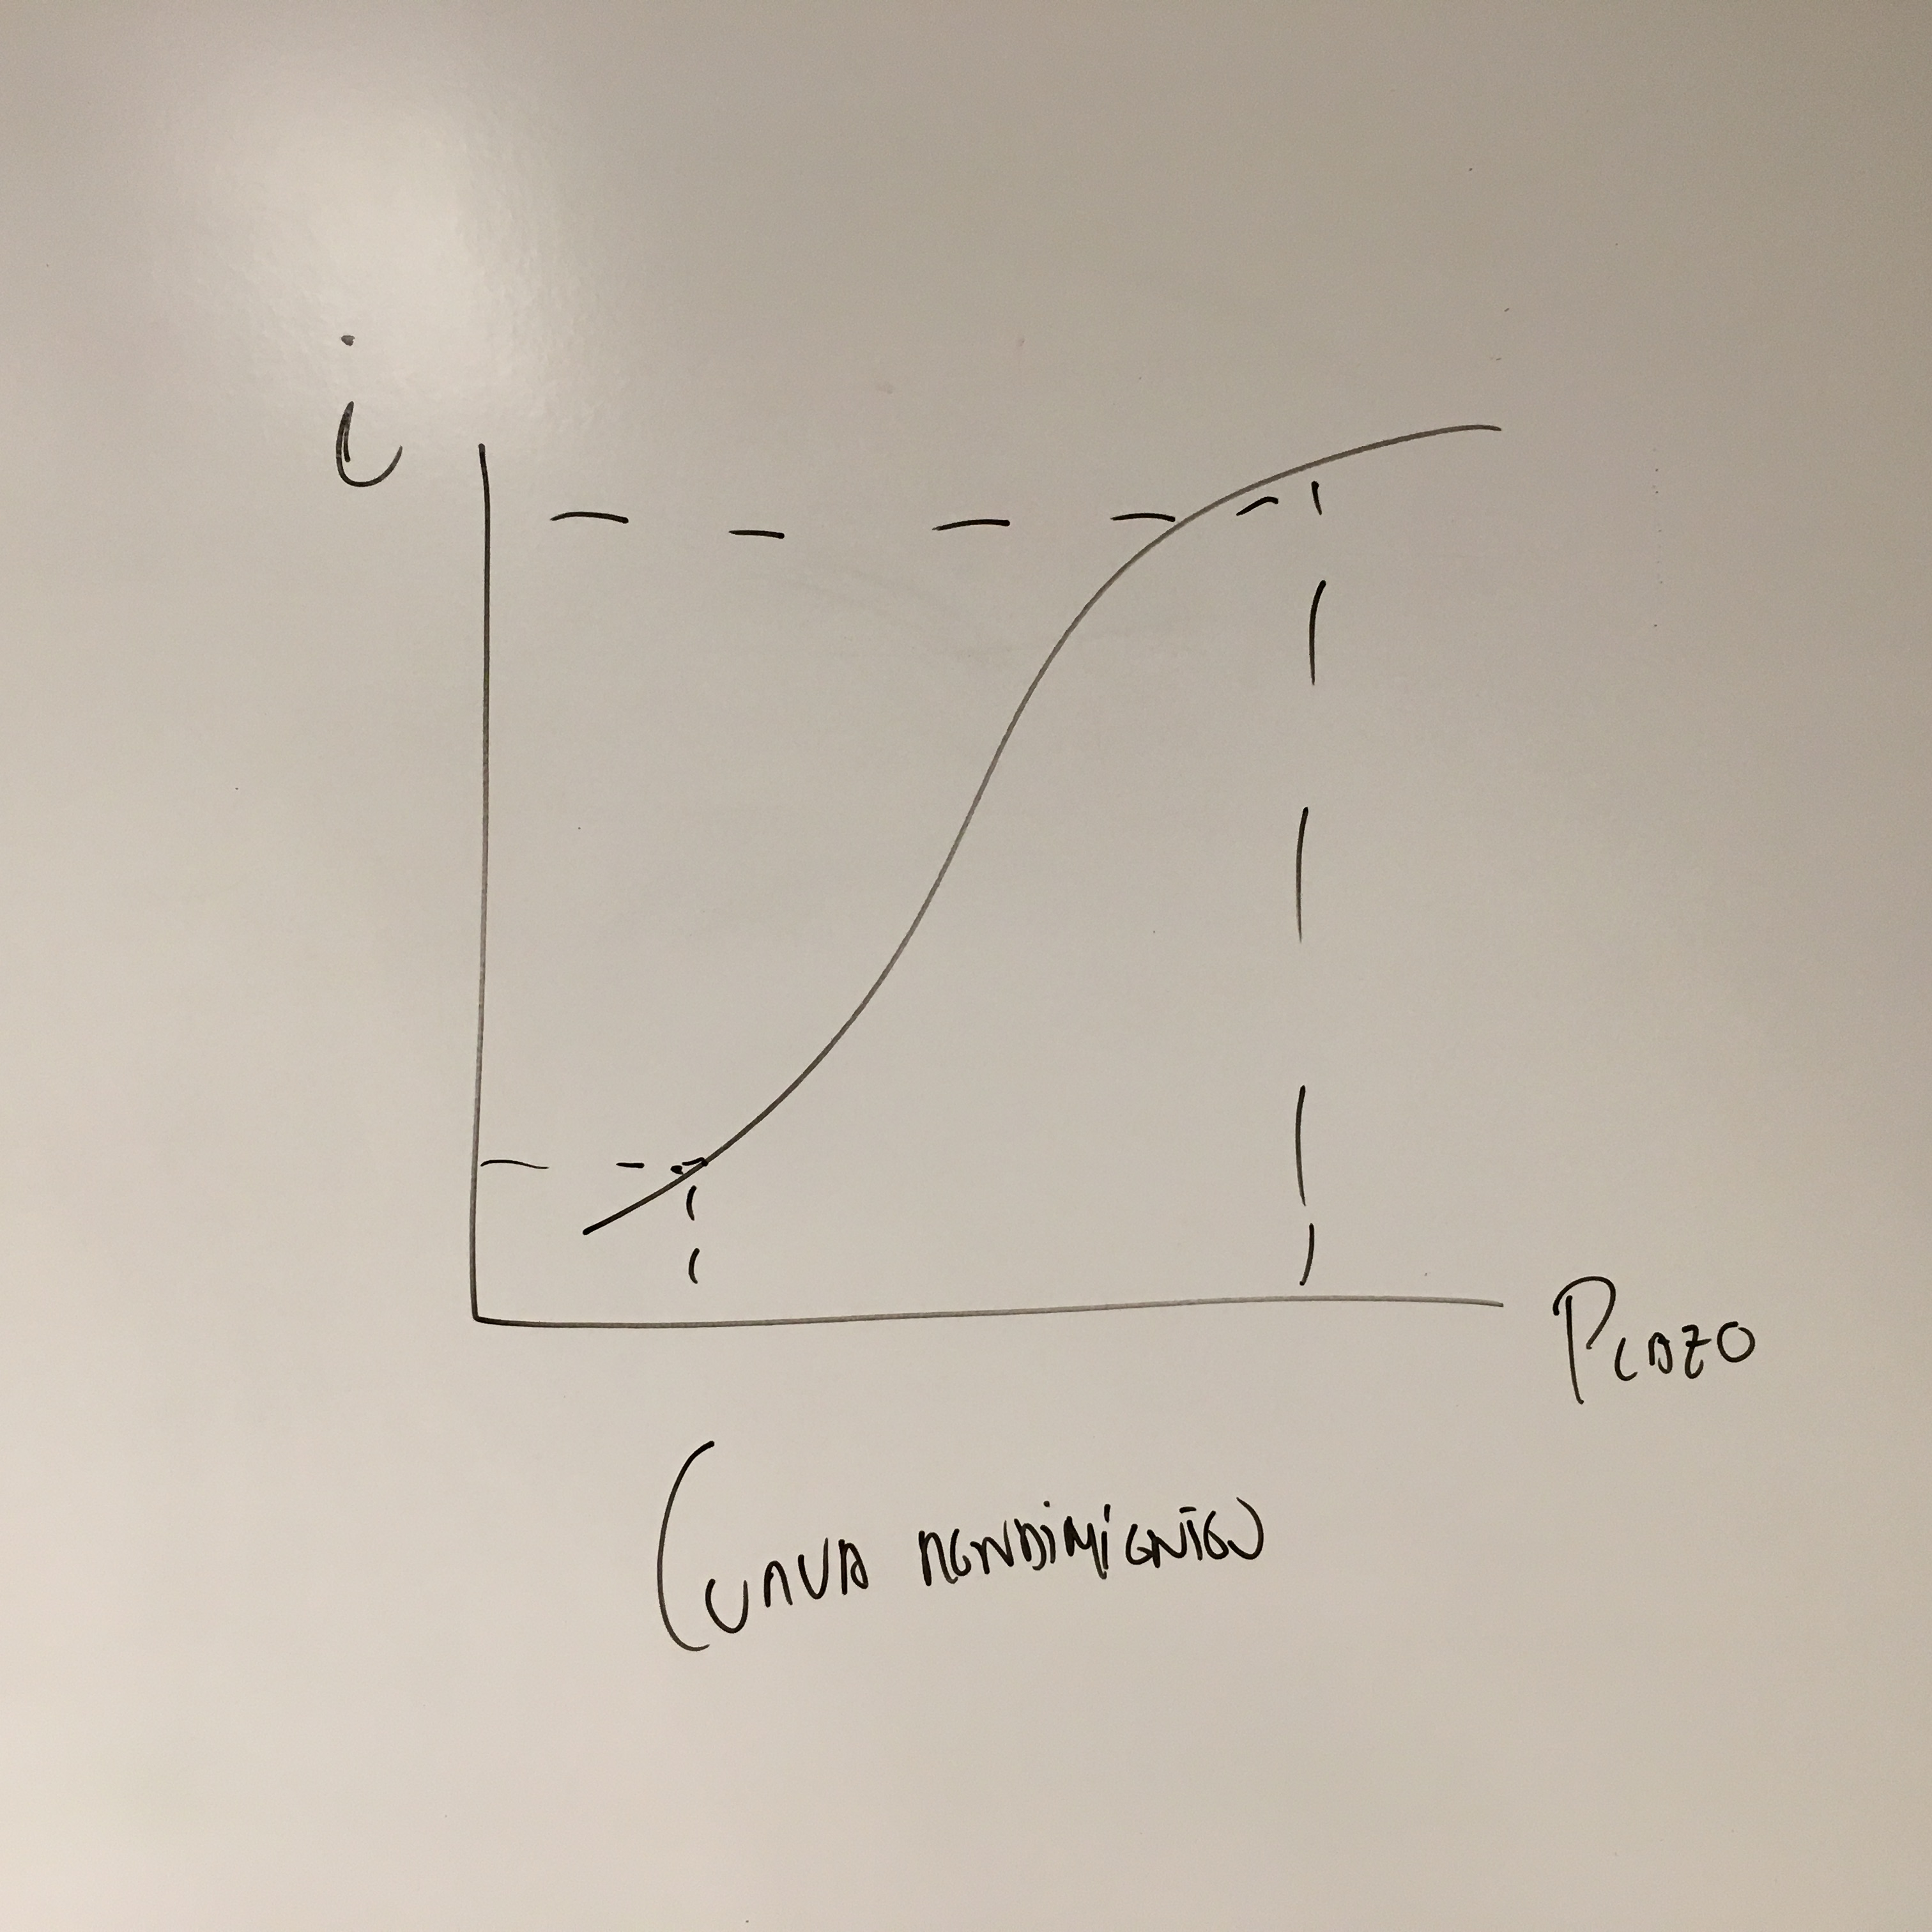
\includegraphics[width=6cm]{Classes/Images/2019-11-04-01.JPG}  
                \caption{}
                \label{}
            \end{figure}              
            \end{center}
        \end{itemize}
    
    \item Banca: comercial y de inversión:
        \begin{itemize}
            \item \emph{\textbf{Definición de ``Comercial":} aquel banco que acepta depósitos del público y da prestamos minoristas a los propios clientes que hacen los depósitos, usualmente prestamos al consumo y prestamos comerciales, hipotecas se consideran prestamos minoristas.}
            \item \emph{\textbf{Definición de ``Inversión":} Leman brothers era un banco de inversión, el banco de inversión no acepta depósitos, y da prestamos mayoritas (usualmente bonos).} \emph{\textbf{Ejemplo: }un banco de inversión le da prestamos a empresas (bonos), el banco de inversión emite deuda,  }
        \end{itemize}
        \begin{center}
        \begin{tabular}{ | p{7cm} | p{7cm} | }
            \hline
            \multicolumn{2}{|c|}{Bancos de inversión} \\
            \hline
                Préstamos (bonos) a empresas  & Deuda de banco (Bonos) \\
            \hline
        \end{tabular}
    \end{center}

    \item Peculiaridades de bancos inversionistas: 
        \begin{itemize}
            \item El banco de inversión: \emph{\textbf{Ejemplo: }ford quiere sacar un nuevo carro, el banco de inversión absorbe la deuda pendiente de ford emitiendo deuda, estos bancos no manejan cuentas individuales.}
            \item Esto pasa mediante bonos.
            \item Esta actividad se llama \emph{dealer} por esto gana interés. Tiene otra actividad que se llama \emph{broker} que básicamente es sentar a los de ford y a la gente que quiere invertir, el banco solo coordina, el banco les cobra a los dos por sentarse en la misma mesa por comisión.  
            \item El banco no es nada más que un comerciante de deudas.
            \item Es la versión bancaria de un fondo de capitales.
            \item \emph{\textbf{Consultar el siguiente recurso:} Fondos del mercado monetario, son casi depositos.}
            \item La banca central no regula estos bancos, a estos los regula otra entidad.
        \end{itemize}
\end{enumerate}





%%%%%%%%%%%%%%%%%%%%%%%%%%%%%%%%%%%%%%%%%%%%%%%%%%%%%%%%%%%%%%%%%%%%%%%%%%%%%%%%%%%%%%%%%%%%%%%%

\end{document}
